%!TEX root = ../template.tex
%%%%%%%%%%%%%%%%%%%%%%%%%%%%%%%%%%%%%%%%%%%%%%%%%%%%%%%%%%%%%%%%%%%
%% chapter1.tex
%% NOVA thesis document file
%%
%% Chapter with introduciton


\chapter{Design and Implementation}
\label{cha:design_and_implementation}

The design process adopted was an iterative design approach to build iteratively the solution according to the users' acceptance and feedback retrieved by users test in each iteration. Throughout this chapter, the design and implementation decisions taken in order to reach the final prototype are detailed.

\section{Sketching}
\label{sec:sketching}

Before starting the development of the interface prototypes, which will be future tested with users, some sketches were performed, in order to organize and explore ideas to tackle the existing usability problems. The primary goal expected to attain at the end of this phase is not a functional or complete interface, but a practical idea of what that could be designed in the following prototypes.

Considering the extensive list of problems identified, prioritization was an important aspect taken into account throughout all design phases. The first problem explored was the difficulty to comprehend the database query purpose.

In the existing interface, users do not have a unique and clear view, which can facilitate the comprehension of what data could be fetched from the database through the query presented. As illustrated in Figure \ref{fig:example_of_query_representation}, the users can only see some components of the query at a time, due to the existence of tabs to individualize each type of query components (i.e., a tab for source, filter and sort options). In addition, as can be observed in Figure \ref{fig:ss_existing_layout}, when users open the query, only the query output preview was shown. That was considered a problem in the analysis of the interface for two different points of view:

\begin{itemize}
    \item When the existing interface was tested with users who do not usually use the Platform, they could not easily find the tabs, which increased the chances of guessing wrongly the query purpose, since they have only observed the query output preview. Besides not being an effective understanding technique, it can be even more difficult when the output contains several columns;
    \item The users accustomed to this data tool revealed that is cumbersome to open and navigate between tabs in order to understand the query.
\end{itemize}

\begin{figure}[tb]
    \centering
    \subcaptionbox{Starting point (only the result is visible)\label{fig:ss_existing_layout}}%
      {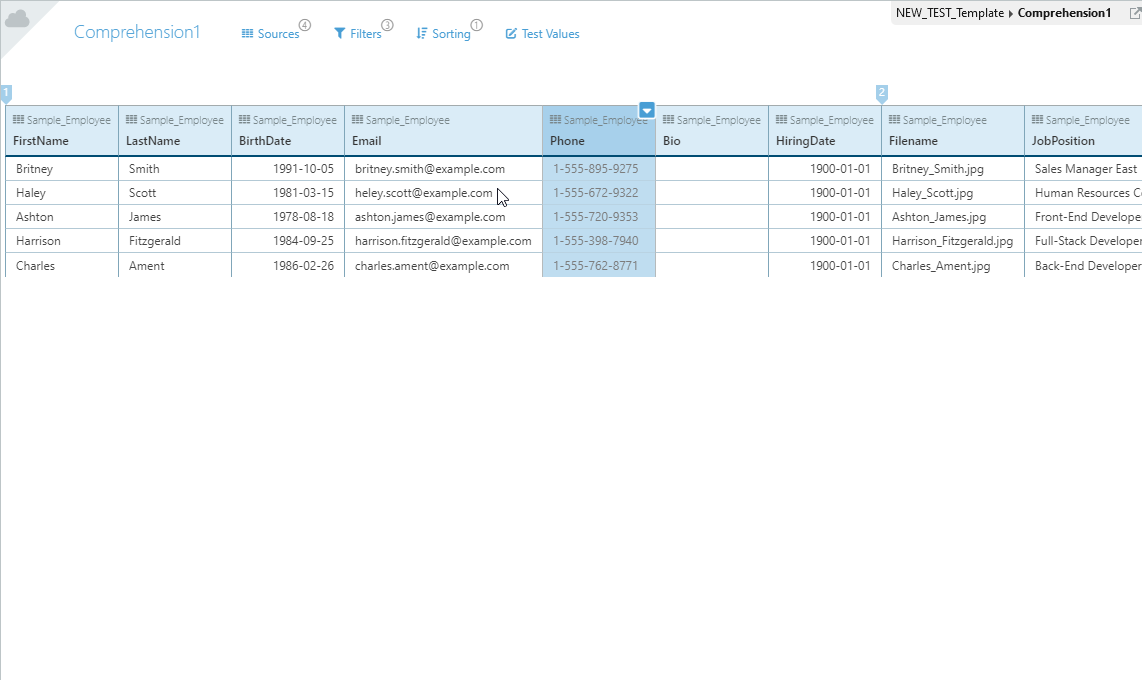
\includegraphics[width=0.5\linewidth]{ss-existing-layout}}%
    \subcaptionbox{Sources Tab\label{fig:ss_existing_layout_sources}}%
      {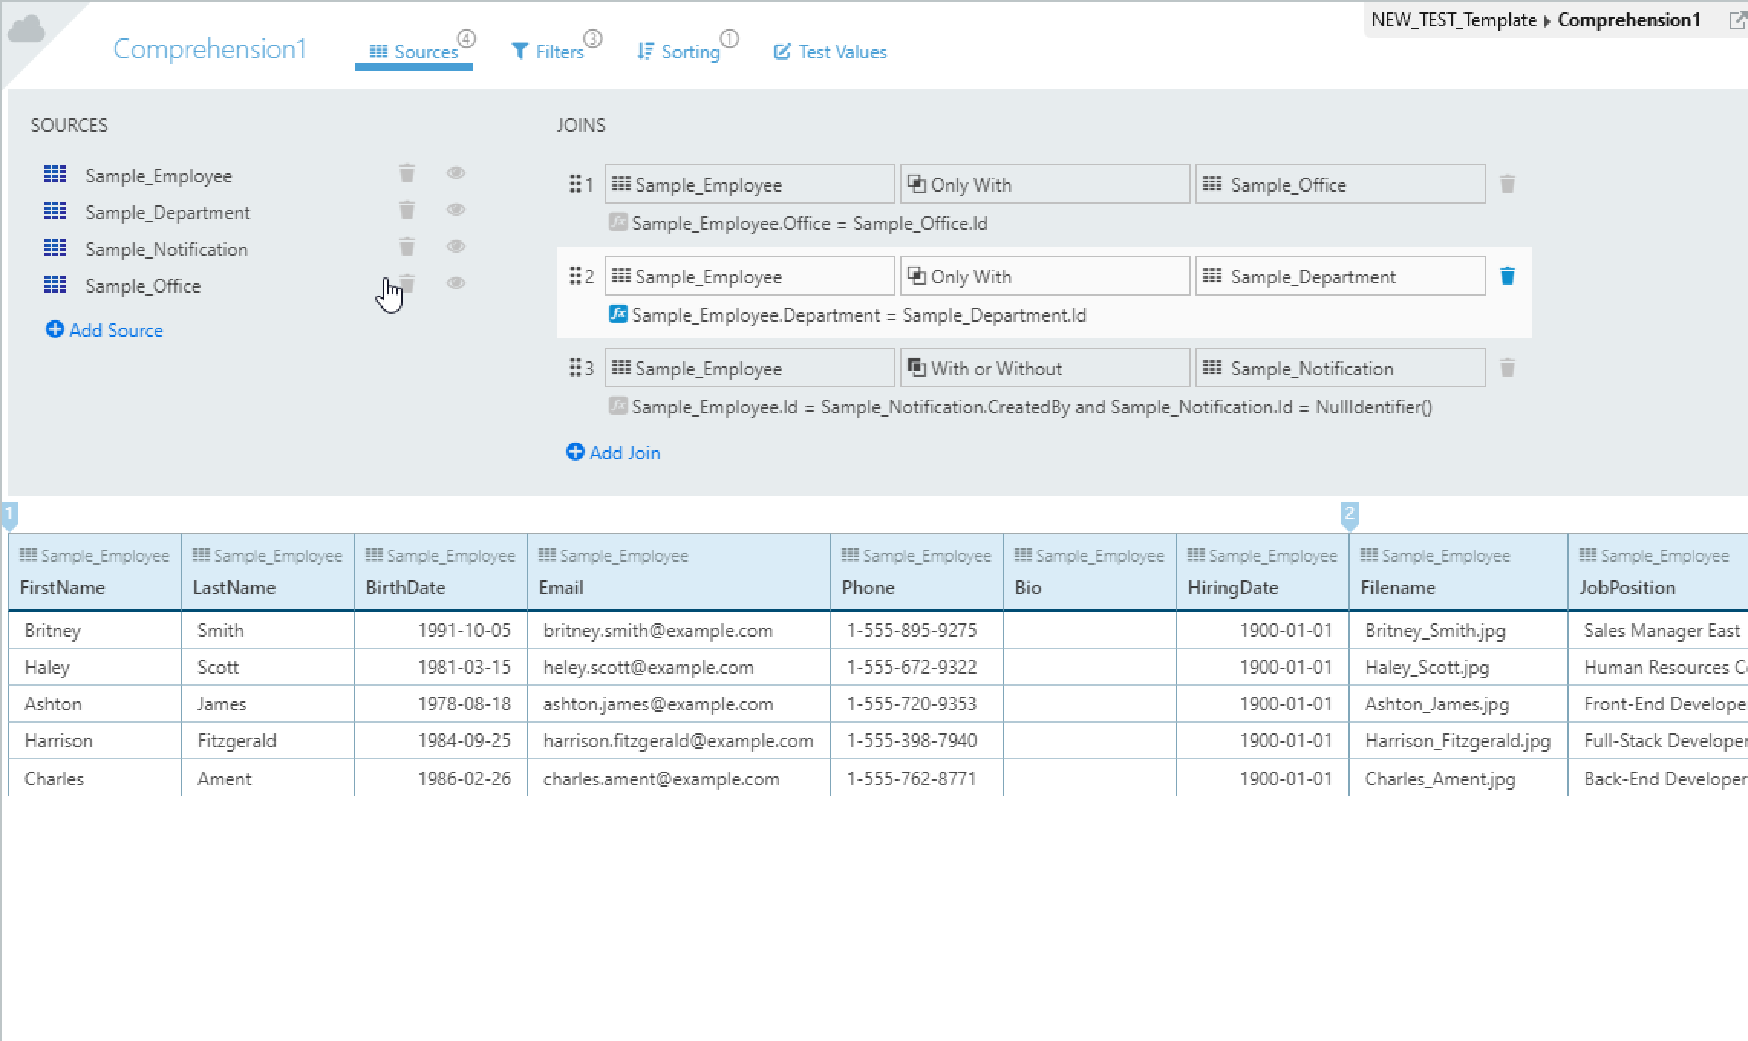
\includegraphics[width=0.5\linewidth]{ss-existing-layout-sources}}%
      \\
    \subcaptionbox{Filters Tab\label{fig:ss_existing_layout_filters}}%
    {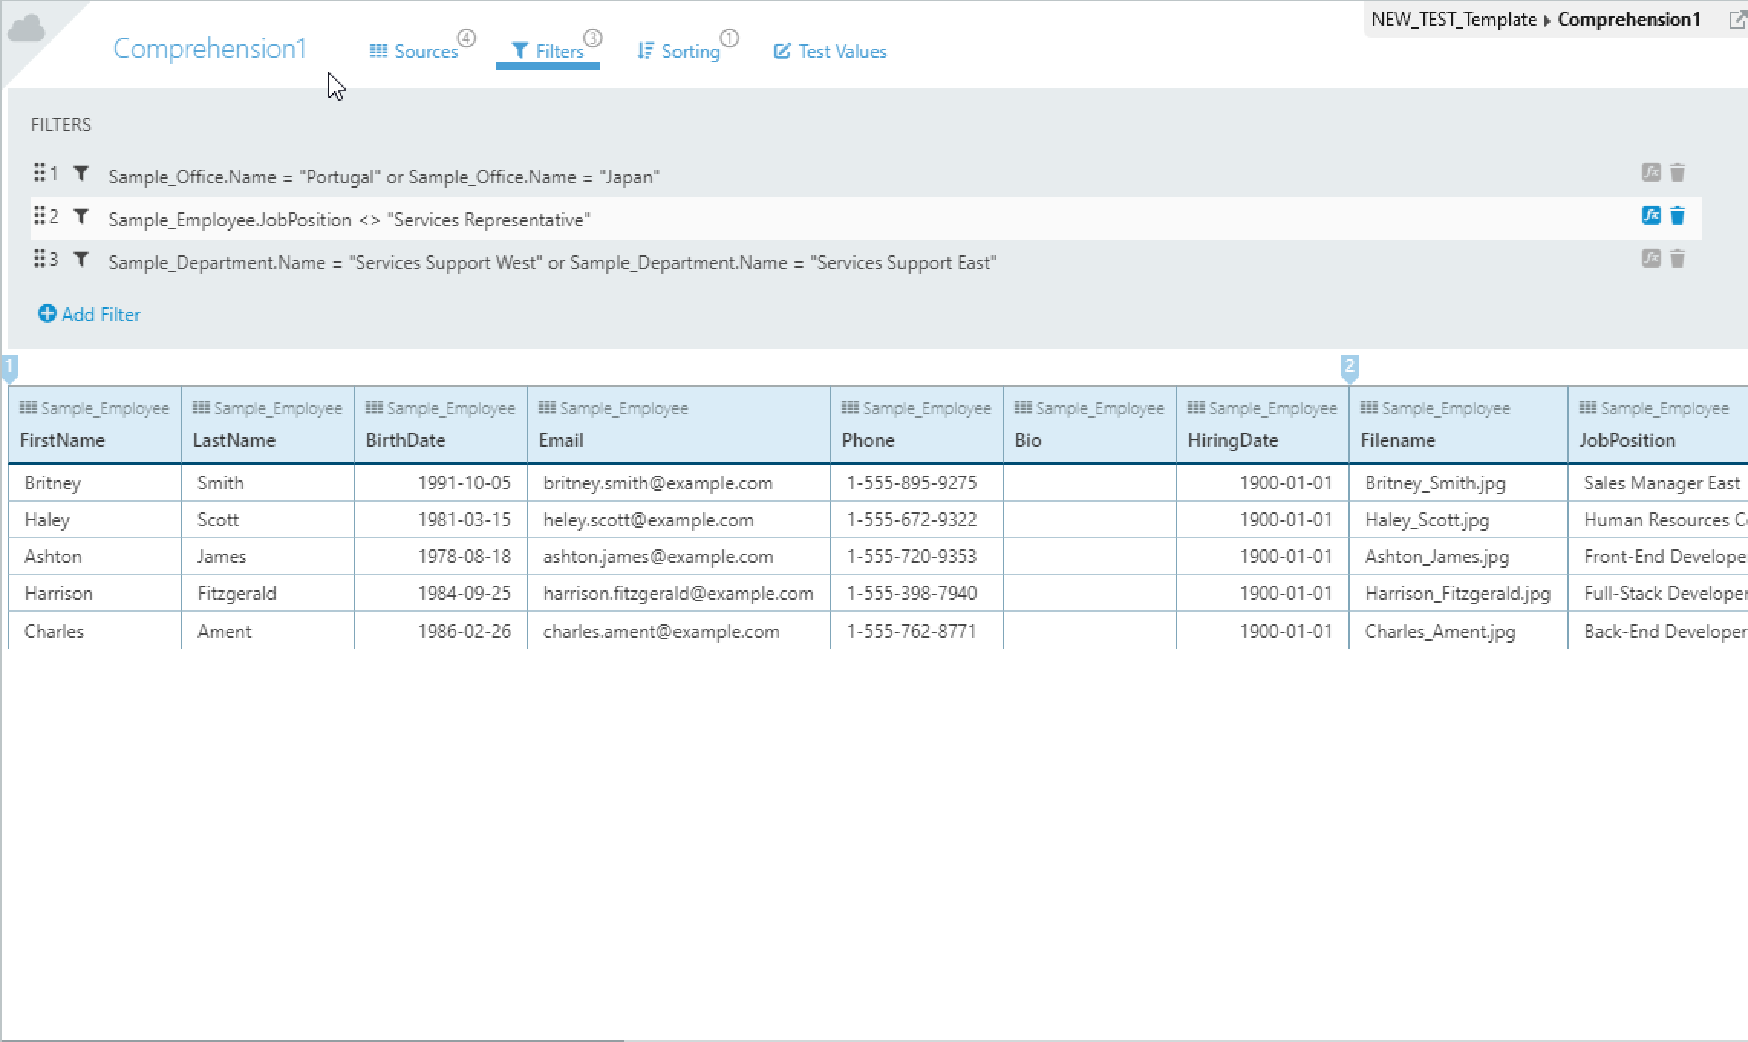
\includegraphics[width=0.5\linewidth]{ss-existing-layout-filters}}%
  \subcaptionbox{Sorting Tab\label{fig:ss_existing_layout_sorting}}%
    {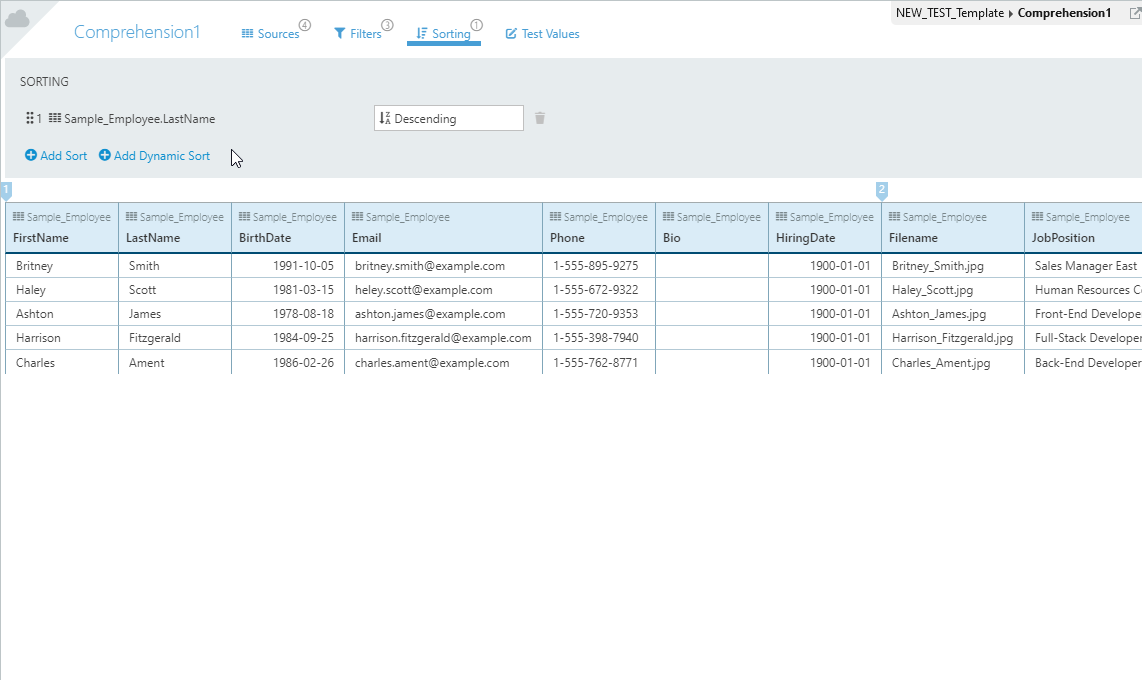
\includegraphics[width=0.5\linewidth]{ss-existing-layout-sorting}}%
  \caption{Example of a database query representation through the existing visual interface.}
    \label{fig:example_of_query_representation}
\end{figure}

Therefore, the designing of a new general layout, where it is possible to view the most important query components at once, was considered a major requirement. A solid improvement regarding this component, could optimize not only the time and effort required to comprehend queries but also to formulate them, since all information is more visible and accessible.

From other prespective, there was also the concern to build a layout that would not compromise the system usability for more complex cases, such as queries that contain a relevant number of entities or conditions.

Accordingly, some wireframes were sketched in order to perceive how the query components could be jointly combined in a unique view. Figure \ref{fig:sketch_wireframes} illustrates the two options elected from multiple approaches explored.

In both options, there are two principal areas in the interface as presented in the current version of the interface: the query editor area and the preview of the query result. Yet, two new manners were explored to display all information of editors jointly with the query result preview. In \nameref{fig:sketch_wireframe_a}, the sub-editors remained in the top area and the query result preview below. The \nameref{fig:sketch_wireframe_b} illustrates another sketched possibility where all editors were presented on the left side of the screen and the visualization of the results presented on the right side.

\begin{figure}[tb]
  \centering
  \subcaptionbox{Option A\label{fig:sketch_wireframe_a}}%
    {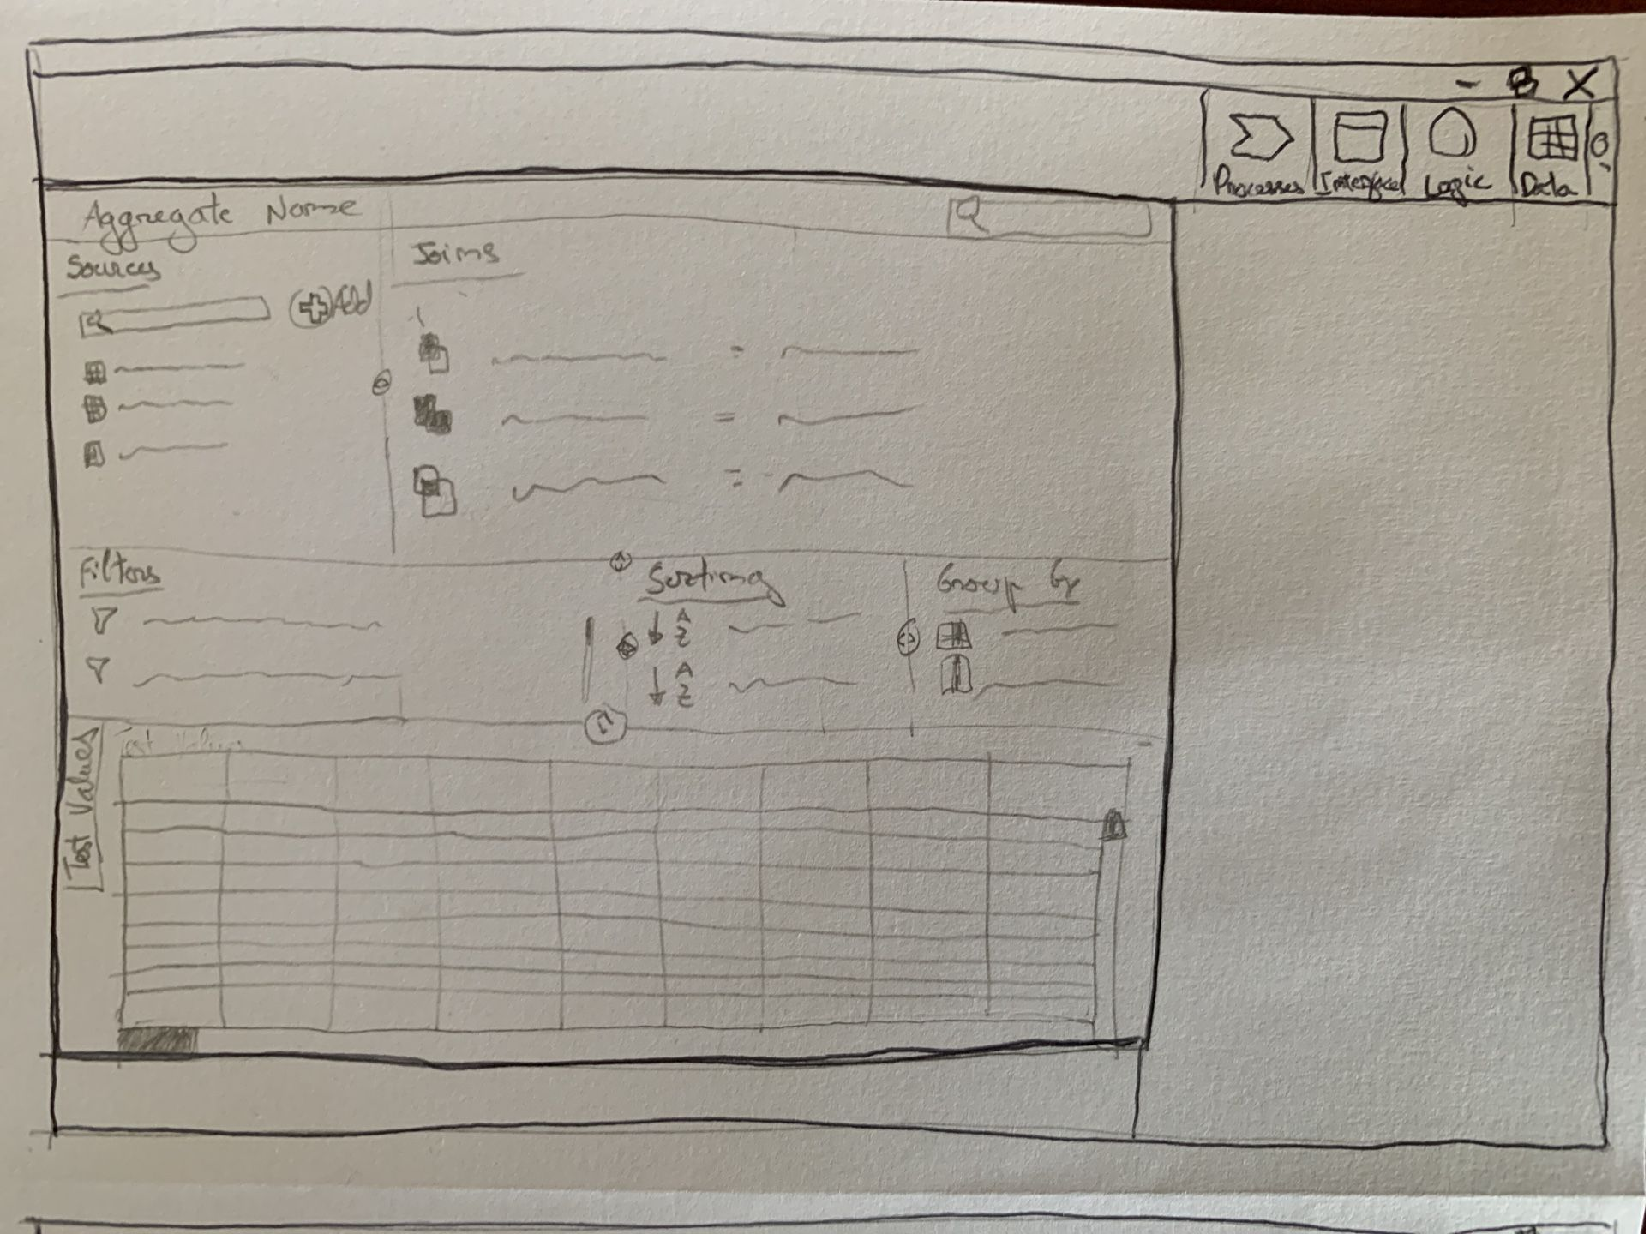
\includegraphics[width=0.5\linewidth]{sketch-wireframe-a}}%
  \subcaptionbox{Option B\label{fig:sketch_wireframe_b}}%
  {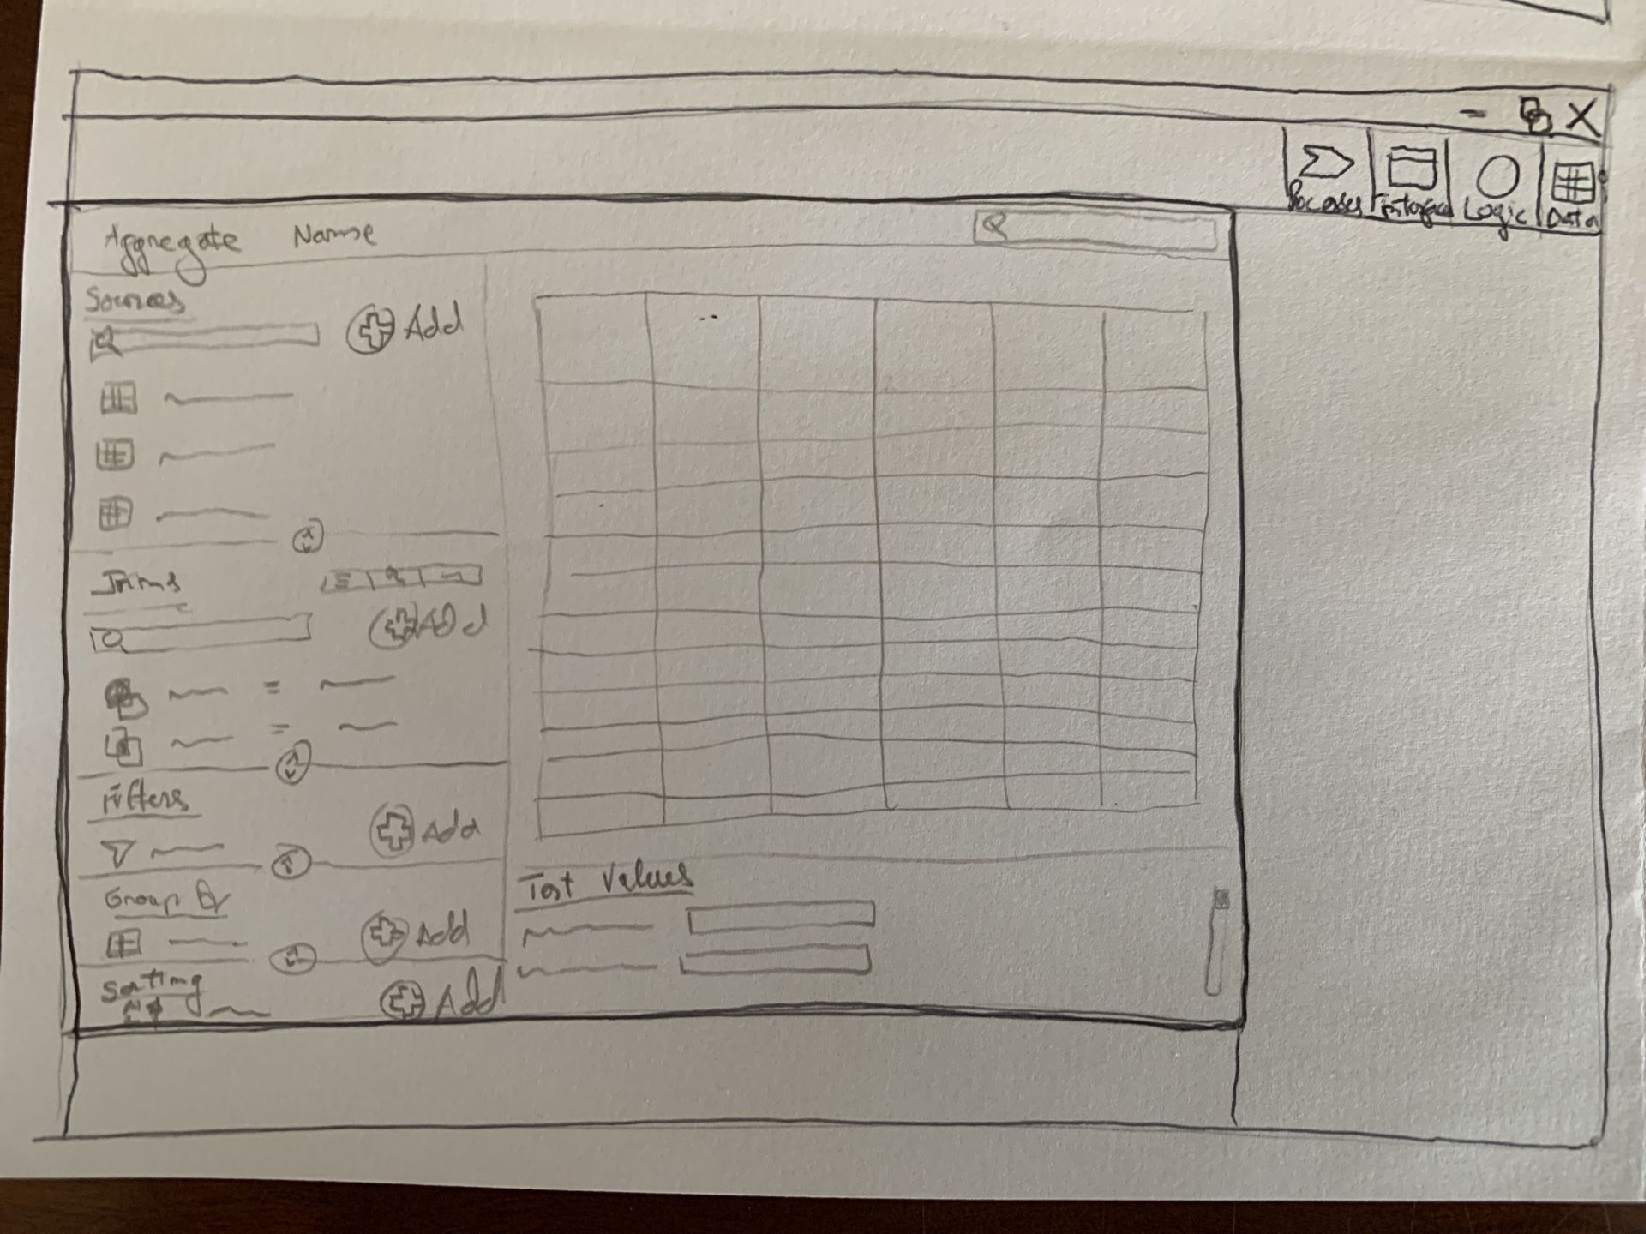
\includegraphics[width=0.5\linewidth]{sketch-wireframe-b}}%
\caption{Interface layout sketches.}
  \label{fig:sketch_wireframes}
\end{figure}

Regardless of the option, the layouts presented have in a single view the most important aspects to understand what query is built.

The existing interface does not have any mechanisms that allows the user to easily find an entity or attribute. The attributes included in the query are not represented in any region of the interface beyond the query result table. Thereby, the unique way to find out the attribute is to look for it in the table header of the query output, using the horizontal scroll. That process is cumbersome and slow, so an alternative was sketched in order to include the attribute in the sources view. The users could click on the attributes and the attribute would be automatically highlighed in the query result preview, as illustrated in Figure \ref{fig:sketchAttributeSearch}. The idea of a search engine was also considered to prompt users to search for an entity or attribute.

\begin{figure}[htbp]
	\centering
	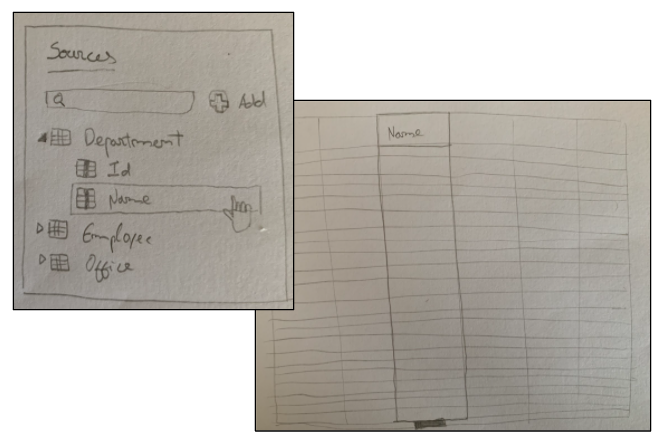
\includegraphics[height=2.5in]{sketch-attribute-search}
	\caption{Searching for an attribute data on the query output preview.}
	\label{fig:sketchAttributeSearch}
\end{figure}

Furthermore, other approaches, more compact and functional, were also explored in order to display the joins used in the query. Figure \ref{fig:sketchJoins} shows the sketched ideas to represent joins: a simple list of all join operations inside the query, and two other ones aggregated by the entities involved by the join kind.

\begin{figure}[tb]
  \centering
  \subcaptionbox{Joins flat list\label{fig:sketch-joins-list}}%
    {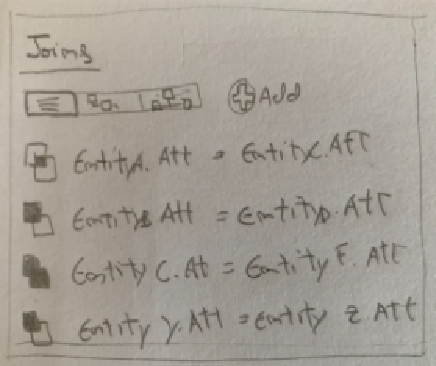
\includegraphics[width=0.3\linewidth]{sketch-joins-list}}%
  \subcaptionbox{Joins associated to each entity\label{fig:sketch-joins-by-entity}}%
  {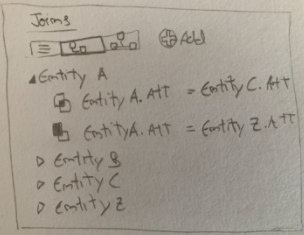
\includegraphics[width=0.3\linewidth]{sketch-joins-by-entity}}%
  \subcaptionbox{Joins by each join kind\label{fig:sketch-joins-by-kind}}%
  {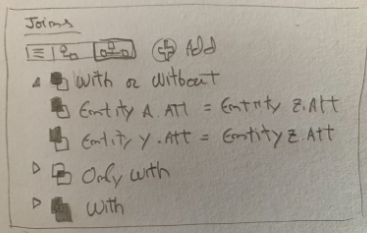
\includegraphics[width=0.3\linewidth]{sketch-joins-by-kind}}%
\caption{Sketches elaborated to explore other approaches to represent the join operations present in the query.}
  \label{fig:sketchJoins}
\end{figure}

Lastly, an idea to accelerate the searching process of a specific element inside the query was sketched. The sketch represented in Figure \ref{fig:sketchGeneralSearch} exhibits an idea, taken into account, to find all references of an entity. This general search would allow users to find entities, joins, filters, or other query elements faster.

\begin{figure}[htbp]
	\centering
	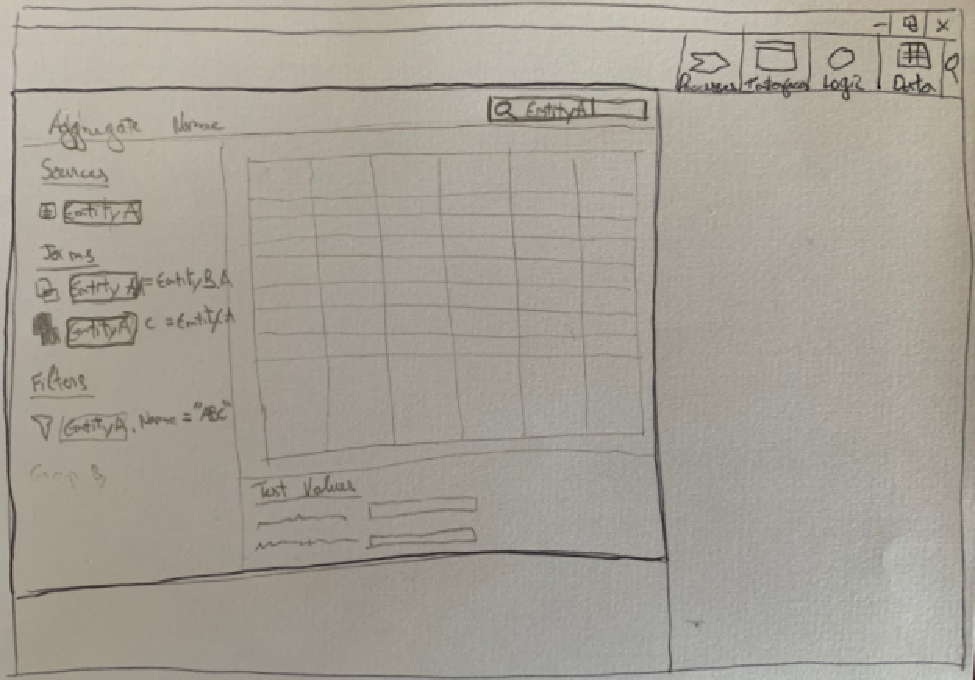
\includegraphics[height=2.5in]{sketch-general-search}
	\caption{Sketch of a general search to allow users to find query elements represented in the interface.}
	\label{fig:sketchGeneralSearch}
\end{figure}


\section{Paper Prototype}
\label{sec:paper_prototype}
The interactive design process started entirety with the first prototype developed: the paper prototype. The main goal of this phase was to build a functional prototype using paper, ruler, try square, and writing materials, in order to create faster and with a low-risk level (i.e., reduced implementation effort spent) a prototype that could be tested by users.

However, due to the COVID-19 pandemic, the prototype was virtually adapted, since it was not possible to test the prototype in person. Accordingly, the prototype was scanned and the interactions were configured using the digital product design platform InVision \cite{invision}.
% Do not forget to refer that due to COVID-19 the Paper Prototype was scanned and assembled as a low-fidelity prototype using InVision App.

\subsection{Design}
\label{subsec:paper_prototype_design}
The building process of this low-fidelity prototype started with the design phase, where a brainstorming of ideas, explored previously, took place, in order to establish the design priorities for the paper prototype as well as concrete ideas to apply in the solutions.

\medskip

\textbf{Sub-editors arrangement:}

\medskip

Taking into account the sketches mentioned in the last section, the first question evaluated was which rearrangement of the sub-editors and the result preview views would be implemented in the next phase. In order to take action in this regard, there was a point in the visual query builder background considered. As mentioned in \ref{subsubsec:previous_work}, this querying interface was completely redesigned seven years ago, which had a negative repercussion on users since they were accustomed to the previous interface. Therefore, there was a concern to change the interface without removing the main points that characterize and identifies it. In that way, the goal was to ensure that users consider the new interface as an improved version of the existing one, instead of a completely different interface.

Comparing the two options sketched (Figure \ref{fig:sketch_wireframes}) with the existing interface (Figure \ref{fig:example_of_query_representation}), the \nameref{fig:sketch_wireframe_a} is the most similar because the editors area keeps on the top region of the interface and the query result data below. For this reason, this arrangement was considered to be presented in the next phase.

Having chosen where would take place the edition area of the interface, the second aspect taken into consideration was how to organize its sub-editors. This decision was taken, bearing in mind, what each query aspect represents in the user's mental model when they formulate queries as well as the physical space of the interface they could occupy.

In this regard, it was thought about what were the order by each query elements arise in user thinking. This reasoning was performed taking into consideration the formulation using \gls{SQL} since one of the main goals is the improvement of the interface experience for users that are proficient in \gls{SQL}. According to the conceptual models presented in \ref{sec:query_conceptual_models}, the first aspect the user thinks, after understanding what data is required, was assessed to be how to translate them to the query language. In \gls{SQL}, the core statements are presented in the following order:

\begin{enumerate}
  \item \textbf{SELECT: }Indicates which attributes will be selected to be present in the query output table;
  \item \textbf{FROM: }Sets out which entities are used to query data. Thereby, even it is necessary to merge tables, the join operations are specified through that statement;
  \item \textbf{WHERE: }Contains the boolean conditions that would filter the results.
  \item \textbf{ORDER BY: }Specify the criteria to order the data gathered.
\end{enumerate}

In this visual query building tool users do not select attributes because there is an optimizing background task that will inspect where the query is used and only select the attributes that will be used. Therefore, in this system, the information specified through the SELECT statement will not be specified by the user.

However, the three other aspects of the query are clearly specified by users in three different interface areas: Sources, Filters, and Sorting respectively. Accordingly, the arrangement chosen to display these three sub-editors, the following logic was considered: the query edition area were divided into two columns, the left side was elected to represent the sources of the query and the right side lists the filters and sorting criteria.

\medskip

\textbf{New approach to represent sources and joins:}

\medskip

Nevertheless, the way entities and joins were presented in the interface, in the previous sources tab, required to be redesigned from scratch. As can be observed in Figure \ref{fig:ss_existing_layout_sources}, a simple list of the entities used was presented in the left side of the editor area and the joins used to merge them in its right side.

Even though some designs regarding that were elaborated in the sketching phase (Figure \ref{fig:sketchJoins}), it was concluded that the main issues remain:

\begin{itemize}
  \item Difficulty to comprehend, fast and with a low-effort, what entities were integrated into the query. Being a visual interface, the comprehension of the entities used as source to formulate the query should be easier to understand. However, the potential of the visual interface has not been leveraged, mainly due to the following aspects:
  \begin{itemize} 
    \item \textbf{Textual language overloading: }Not only all join conditions were completely presented in full-textual way, but also the same entity could be written in a repeated way. For example, in the example shown in Figure \ref{fig:exampleTextualLanguageOverloading}, the entity $"Sample\_Employee"$ was presented seven times to indicate that the query uses this entity and this entity was joined with three other entities;
    \item \textbf{Lack of guidance to understand what entities are related to each other: }As the entities and sources are listed in the interface, the design should help users to understand which entities are joined. For instance, if joins were put between the entities involved, it would be simpler to identify if they were merged through a join operation.
  \end{itemize}
  \item The users who are not familiarized with relational databases and the terminology used to join tables pointed out that the existing view is complex and difficult to understand.
\end{itemize}

\begin{figure}[htbp]
	\centering
	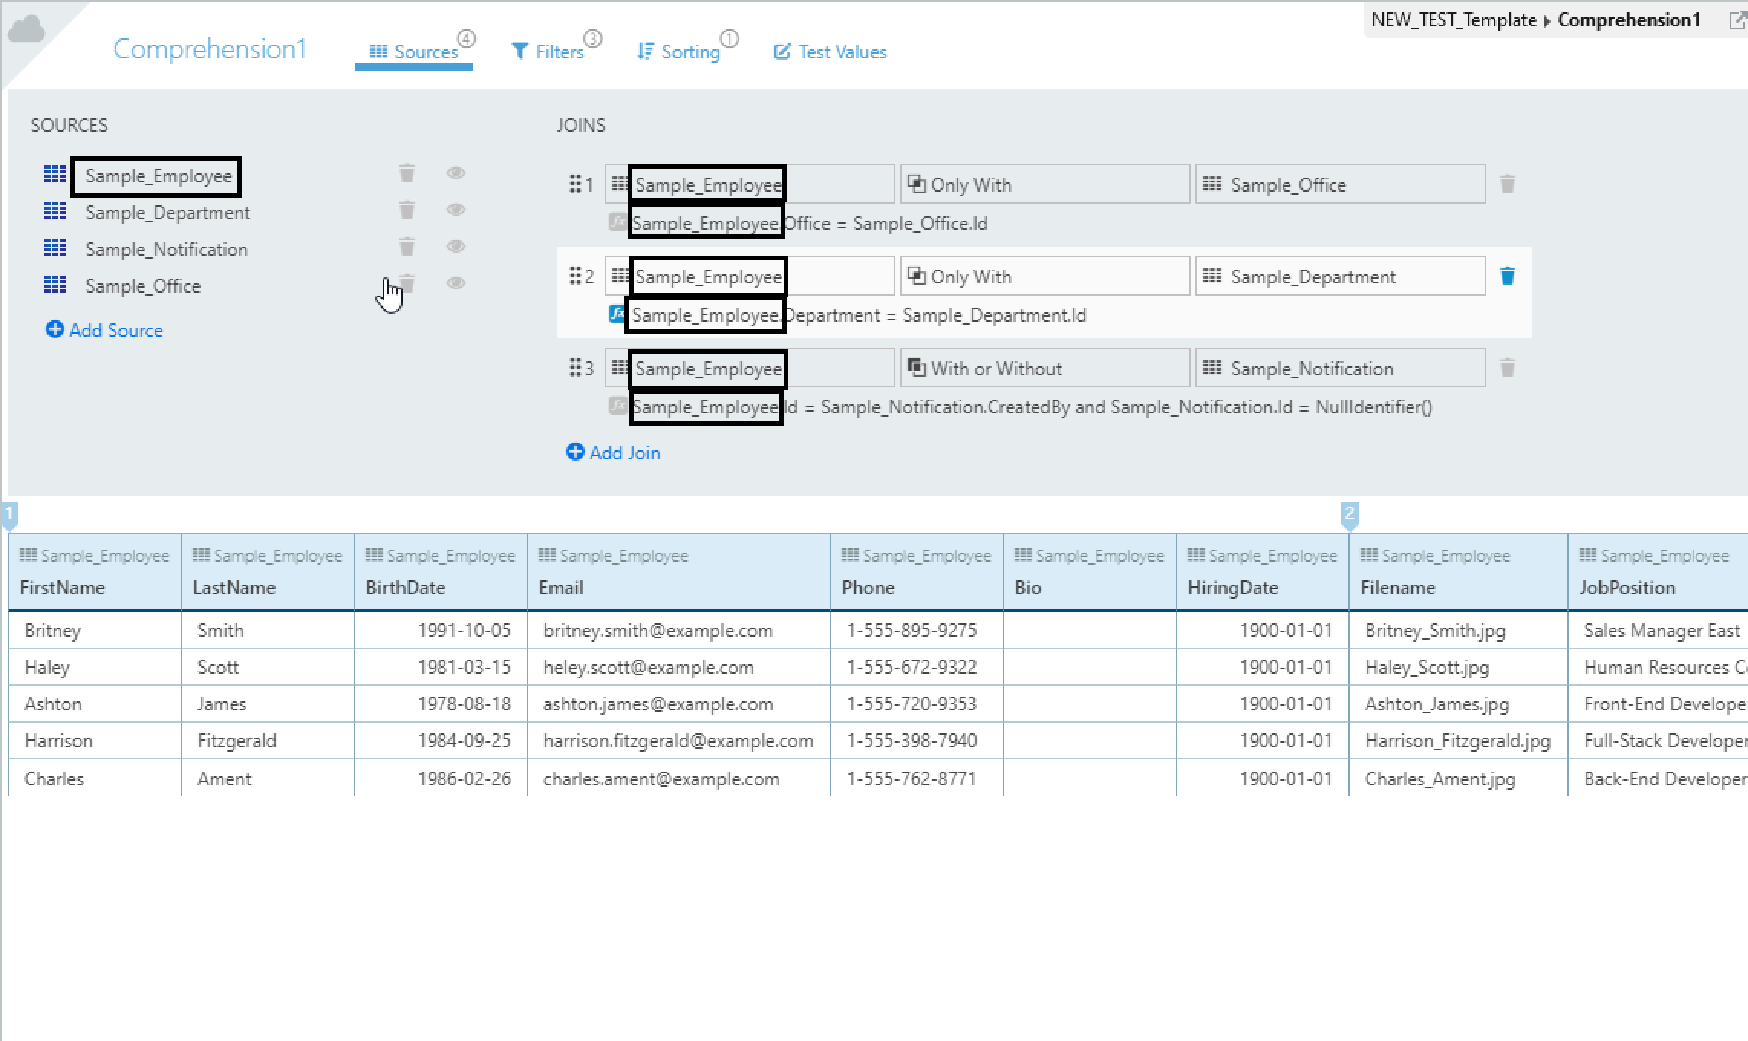
\includegraphics[height=2.7in]{example-textual-language-overloading}
	\caption{Example of the existing textual language overloading - The entity $"Sample\_Employee"$ is represented seven times. }
	\label{fig:exampleTextualLanguageOverloading}
\end{figure}

Therefore, the way entities and joins were listed in the sources tab of the existing interface was reconsidered, since it was intended to create a simpler, intuitive, and compact viewing area.

The idea of a tree view which displays all entities and joins used in the query has emerged to tackle the problem mentioned. Through that approach, it would be possible to reduce the entity repetition and to explicitly perceive which entities have a certain entity been joined.

\medskip

\textbf{Query formulation improvements: }

\medskip

%learnability
Regarding query formulation, there was several users who are not accustomed to the query builder, meaning that they appeared to have difficulty to discover some functionalities of the system when they were testing the existing interface. Thereby, learnability was also considering during the design phase of the first prototype.

As mentioned in \ref{subsec:analysis}, the options to add a new calculated attribute or to apply a group by or aggregation functions were hidden. These functionalities could be frequently used, thus it was concluded that these options should be visible in the sources area. By doing this, not only the options were still visible to the novice users but users could have a faster alternative to insert these query components.

%efficiency

Lastly, the distribution of the formulation options (i.e., the buttons or other interface elements that allow users to insert new elements in the query) in the screen was a relevant aspect considered.

The main concern was to put these controls near to the area where the content will be displayed. As an example, if there is an area where entities, joins, and attributes are placed together, the related interaction should be accessible near them. In that way, users do not need to find options in other areas of the interface, keeping the user task on track, avoiding them to lose reasoning context.

That design principle was considered advantageous to reduce the user's working memory overload since they could focus in each part of the query without distractions. Moreover, if the controls are near, the time the mouse need to move to them, is also reduced, accelerating the query formulation process.

%Falar da divisão e distribuição do layout
%Falar que tendo em conta o espaço disponível seria necessário encurtar a representação das sources e joins.
%Adicionar fatores diferenciadores para a leitura da query: color highlighting nos filters, melhorar a leitura dos dados na tabela dos resultados, adicionar opções mais visíveis e acessíveis (práticas, rápidas) para adicionar novos attributos.

%Para além disso, foi mais tido em conta a preocupação de colocar numa sub região da interface a maior parte dos controlos mais utilizados, de modo a formulação da query poder ser realizada de forma mais rápida e eficaz, visto que não só se diminui o tempo através da menor distância que o rato tem que percorrer, como também porque o  utilizador vai mantendo o mesmo contexto visual.


\subsection{Implementation}
\label{subsec:paper_prototype_implementation}

After defining priorities for the current design iteration, the paper prototype implementation has launched. In this phase, the pieces of the prototype were built progressively considering the key points presented before and refining some details whenever necessary.

\medskip

\textbf{General layout:}

\medskip

As the reasoning applied in the design phase, the general layout was the first part implemented. The main concern at this phase was the definition of the dimensions for each sub-editor. In order to ensure that the design will be properly integrated into the Service Studio, it was created a sketched background image of the \gls{IDE} using a function of Balsamiq \cite{balsamiq} to convert the Service Studio screenshot to a black and white line drawing version \cite{balsamiq_using_images_and_assets}. As a result, it was possible to perceive if the design done would combine with the system where its is integrated without increasing the fidelity level of the prototype.

After that, the main areas of the interface were elaborated until reaching the general layout that can be observed in Figure \ref{fig:paperPrototypeGeneralLayout}.

\begin{figure}[htbp]
	\centering
	\includegraphics[height=3.0in]{paper-prototype-general-layout}
	\caption{Paper Prototype general layout.}
	\label{fig:paperPrototypeGeneralLayout}
\end{figure}

\medskip

\textbf{Query Result Table:}

\medskip

The next step was the design of the query result tables which shows the result preview of the query built. An outuput result table was designed in order to provide, in all user testing scenarios, a real context to users when they tested the prototype.

In order to accelerate the process of the table design in paper, it was used the same Balsamiq functionality used for background, to transform the table of the existing interface into a low-fidelity design.

However, the headers of the table were redesigned manually to improve the readability of the table to optimize the understanding of where data of an entity starts from data of another entity. In that way, the entity reference in the table header were merged to give to the user an easier perception that all the attributes below belong to the entity above. Figure \ref{fig:queryResultTableComparison} compares the existing one to an example of one of the tables built.

\begin{figure}[tb]
  \centering
  \subcaptionbox{Existing Interface\label{fig:queryResultTableComparisonExisting}}%
    {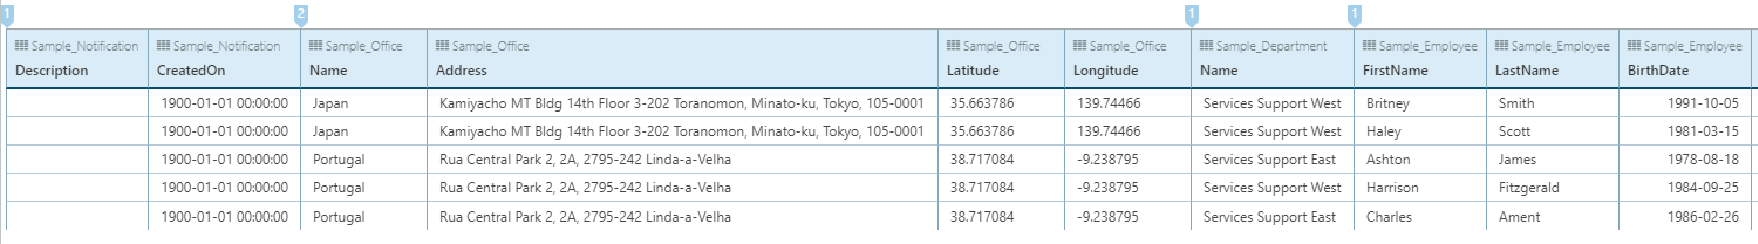
\includegraphics[width=0.9\linewidth]{query-result-table-existing}}%
    \\
  \subcaptionbox{Paper Prototype\label{fig:queryResultTableComparisonPaper}}%
  {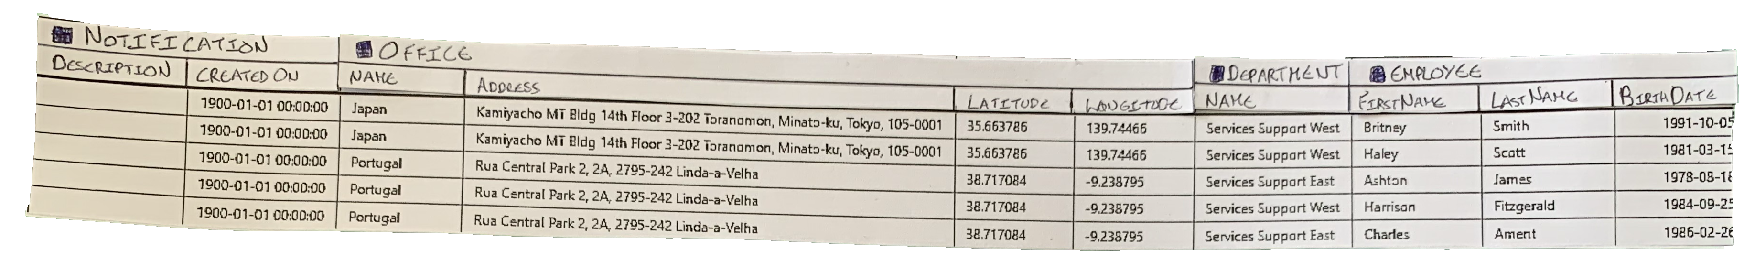
\includegraphics[width=0.9\linewidth]{query-result-table-paper}}%
\caption{Comparison between the existing query result table and the designed for the Paper Prototype.}
  \label{fig:queryResultTableComparison}
\end{figure}

\medskip

\textbf{Filters and Sorting: }

\medskip

Regarding filters and sorting, it was decided to not apply major changes since there were other problems considered as more relevant. Even though the filters edition could be faster using accelerators such as copy and paste or the possibility to edit each filter in the line, instead of opening the expression editor, these problems, as well as other similar problems, mentioned in the Appendix \ref{app:taxonomy_of_problems_existing_interface} - \nameref{app:taxonomy_of_problems_existing_interface}, were not tackled. The reason to disconsider these improvements in the prototyping phase was that there are straightforward improvements that have a low-risk of affecting negatively the user's experience. In that way, it the focus was to the design parts that should be rigorously tested by users to ensure that riskier changes are improving the usability of the interface.

Accordingly, concerning filters, it was only added some syntax highlighting to each one of the conditions presented in order to reduce the time required to understand the conditions. Figure \ref{fig:filtersAndSortingComparison} presents an example of Filters and Sorting design in the paper prototype.

\begin{figure}[tb]
  \centering
  \subcaptionbox{Existing Interface\label{fig:filtersAndSortingExisting}}%
    {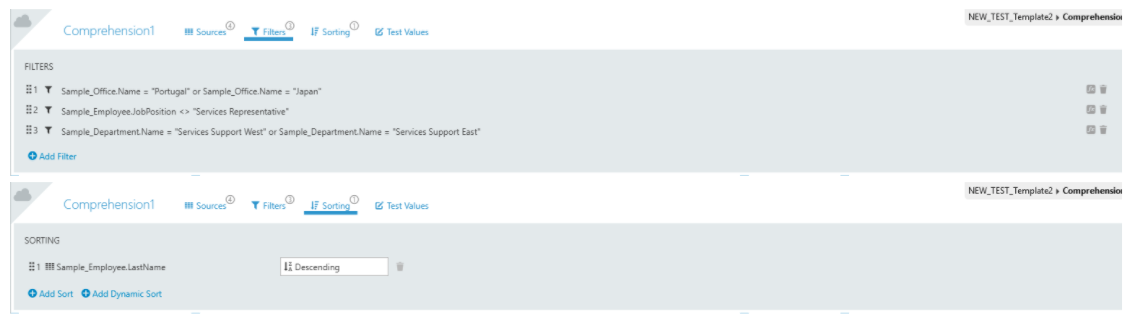
\includegraphics[width=0.9\linewidth]{existing-filters-sorting}}%
    \\
  \subcaptionbox{Paper Prototype\label{fig:filtersAndSortingPaper}}%
  {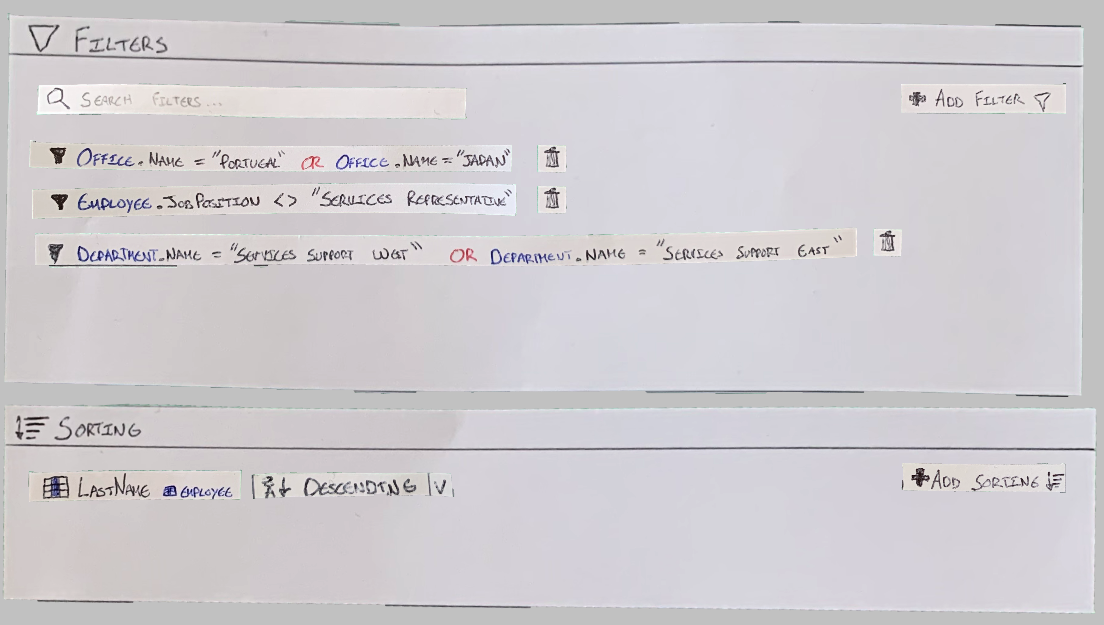
\includegraphics[width=0.9\linewidth]{paper-filters-sorting}}%
\caption{Comparison between the existing filters and sorting sub-editors and the ones designed for the Paper Prototype.}
  \label{fig:filtersAndSortingComparison}
\end{figure}

\medskip

\textbf{Sources View: }

\medskip

As referred before, the design of the sources view was considered one of the most impactful aspects to improve the query builder usability. The restructuration design of this element was reasoned as a crutial section of the interface that could leverge the usability of the system. 

A new approach to represent sources and joins was built progressively. The first aspect approached was the creation of a hierarquical view similar to a tree view which gives to the user the perception of what entities are related with each other. Figure \ref{fig:simpleSourcesTree} shown an example of a tree built at that stage.

\begin{figure}[htbp]
	\centering
	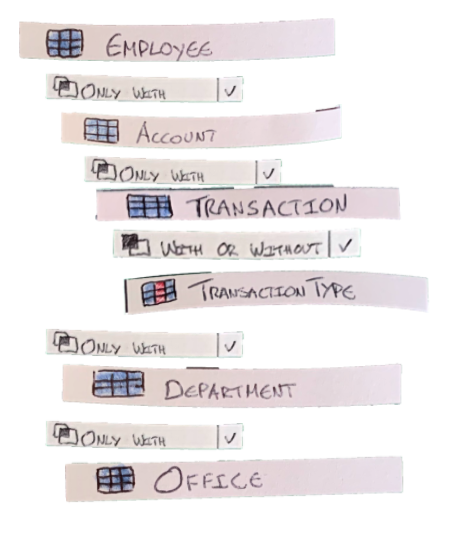
\includegraphics[height=2.7in]{simple-sources-tree}
	\caption{First stage of the design of a new representation approach to display sources and joins.}
	\label{fig:simpleSourcesTree}
\end{figure}

Notwithstanding the visual simplicity achieved was insufficient since it not represents the join conditions. However, if join conditions were just included near to the join type, the interface would be overloaded again and it would still poor readability.

Furthermore, the usability tests of the existing interface showed that users tended to misunderstand the queries that display joins with specific characteristics. In particular, in cases where queries had joins with conditions that contained logical operators or when the join between the two tables could be done through different attributes.

Through practical examples it is easier to understand the dimension of the problem. For example, considering the data model presented in Figure \ref{fig:dataModel}, if a user wants to query the employees and their departments, he will add the two entities and the visual query builder will build automatically the join condition:

\begin{center}
  \verb|"Sample_Employee.Office = Sample_Office.Id"|
\end{center}

This automatism is useful and turns the query formulation process more simple and efficient. However, there are cases where the join needs to be specified. For instance, considering the same data model, if a user wants to query the employees who are owners of accounts, the join condition has to merge the two entities $"Sample\_Employee"$ and $"Sample\_Account"$ using the foreign key $"Owner"$ and not the two other available alternatives: $"CreatedBy"$ and $"Manager"$. In this case the condition required to build this query is:

\begin{center}
  \verb|"Sample_Employee.Id = Sample_Account.Owner"|
\end{center}

In these cases, the join condition, which in many cases is not so important as just covers the general case and it was generated automatically by the system, represents an important aspect of the query. However, as illustrated in the example of Figure \ref{fig:comprehension2JoinsExisting}, the existing interface represents all joins equally.

\begin{figure}[htbp]
	\centering
	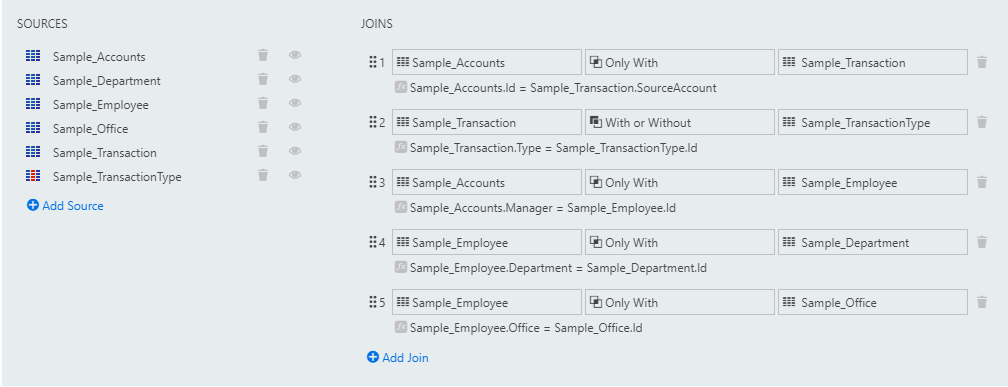
\includegraphics[height=2.2in]{comprehension-2-joins-existing}
	\caption{Example of joins representation in the existing interface in a query where the foreign key used to join is an important detail.}
	\label{fig:comprehension2JoinsExisting}
\end{figure}

When users tested the existing interface with cases similar to the one presented, two relevant usability problems were detected. On the one hand, when users tried to comprehend the query, most of them did not pay attention to this detail, not mentioning the foreign keys used. On the other hand, when they need to formulate queries that contemplates these cases, several users, even the most experienced using this query builder, did not select the intended foreign key. This behavior was considered normal since the system just assumes one of the foreign keys and generate the join, without asking user what attribute he would want to use to join the two entities.

Therefore, the exploration of a new sources and joins representation was an excellent opportunity to tackle this problem. In that way, the existing tree view of sources was designed in order to integrate also the foreign key used to build each of the presented joins. Moreover, when two entities are added and the join between them can be done through different keys, the system starts asking the user which key he wants to use. Figure \ref{fig:paperFkSelect} illustrates how this idea was transposed to the paper prototype.

\begin{figure}[htbp]
	\centering
  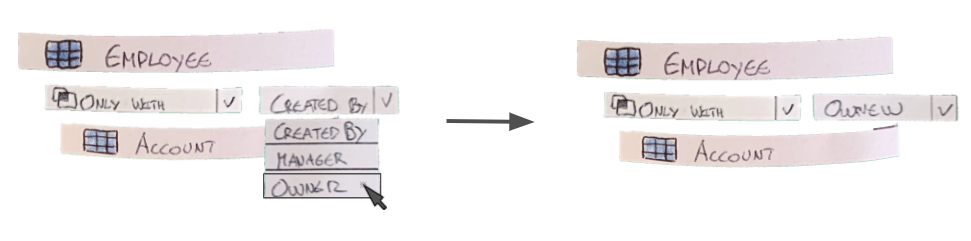
\includegraphics[height=1.4in]{paper-fk-selection}
	\caption{Example of the new foreign key selection and representation applied in the Paper Prototype.}
	\label{fig:paperFkSelect}
\end{figure}

Nevertheless, the foreign key is not the only aspect that could be specified in the join condition. As in SQL, the existing query builder allows user to edit manually the join condition, for example to add more restrictions using logical operators.

In these cases, not only is it important to continue to allow the conditions editing in the new interface but the conditions already edited should also be highlighted in such a way that users who open the query for the first time perceive that the condition of these joins is different. 

The strategy applied in the paper prototype to maintain the interface simple, clear, and intuitive while highlighting the relevant aspects was to put only the function icon in the simple join conditions, and the other ones has their difference explicitly represented after. Figure \ref{fig:paperComprehension1Sources} represents the sources of a query with a join condition edited. In this case the join condition between $"Sample\_Employee"$ and $"Sample\_Notification"$ was changed since the goal is to fetch the employees who have never created notifications. Accordingly, a simplification took place to represent only the differentiating factor instead of the full condition which is:

\begin{center}
  \verb|"Sample_Employee.Id = Sample_Notification.CreatedBy and| 
  \\
  \verb|Sample_Notification.Id = NullIdentifier()"|
\end{center}

\begin{figure}[htbp]
	\centering
  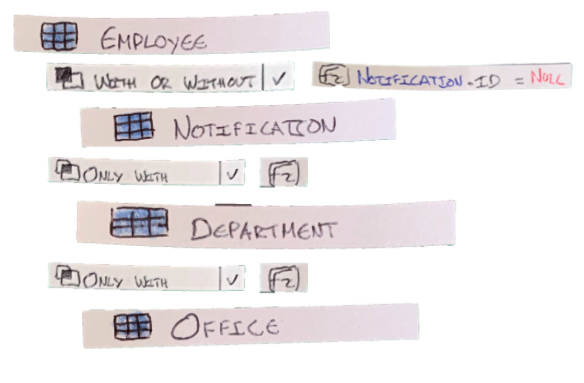
\includegraphics[height=1.4in]{paper-comprehension-1-sources}
	\caption{Example of the sources of a query that has a join with a condition edited.}
	\label{fig:paperComprehension1Sources}
\end{figure}

Through that approach, users will be able to identify entities and joins of the query without information overloading, allowing them to perceive easily and faster the purpose of the query. Even if the join condition is hidden, the user could click on the function icon and the expression editor would appear making possible to see and edit the join condition selected.

\medskip

\textbf{New alternatives to add and search for attributes:}

\medskip

The last improved aspect during the development of this paper prototype was regarding the addition of new attributes. In accordance with the mentioned in the last section, there was a demand to provide other alternatives to add calculated attributes as well as group bys or aggregation functions.

Considering the concern to insert strategically these alternatives, in easily and fast accessible places, it was necessary to improve the visibility of these options to improve the learnability of novice users. The following options were applied:

\begin{itemize}
  \item \textbf{Click and right-click in the attributes exhibited in the Sources sub-editor: }The list of the attributes of each entity was added into each entity represented in the Sources of the query. On the one hand, if users click in an attribute, they would see the data related into the query result preview (according to the sketch already presented in Figure \ref{fig:sketchAttributeSearch}). On the other hand, if they right-click in an attribute, they would see the same context menu that they already could see when they right-click on the result table headers. Therefore they could apply operations using that alternative, as exemplified in Figure \ref{fig:paperAttributeRightClick}.
  \item \textbf{Two new visible buttons to add attributes: }In the footer of the Sources View, two buttons were added:
    \begin{itemize}
      \item \textbf{Aggregation / Group By: }Clicking in this button the user could choose an attribute and apply the following operations to group the data of the attribute: Group by, Sum, Average, Max, Min, or Count. Figure \ref{fig:paperAddAggregation} shows this new formulation area.
      \item \textbf{Calculated Attribute: }When the user selects this option the interface will show an expression edition area similar to the existing one (as exemplified in Figure \ref{fig:calculated_attribute_example}) to indicate the formula of the new attribute. Figure \ref{fig:paperAddCalculatedAttribute} shows this alternative to add a new calculated attribute.
    \end{itemize}
\end{itemize}


\begin{figure}[htbp]
	\centering
  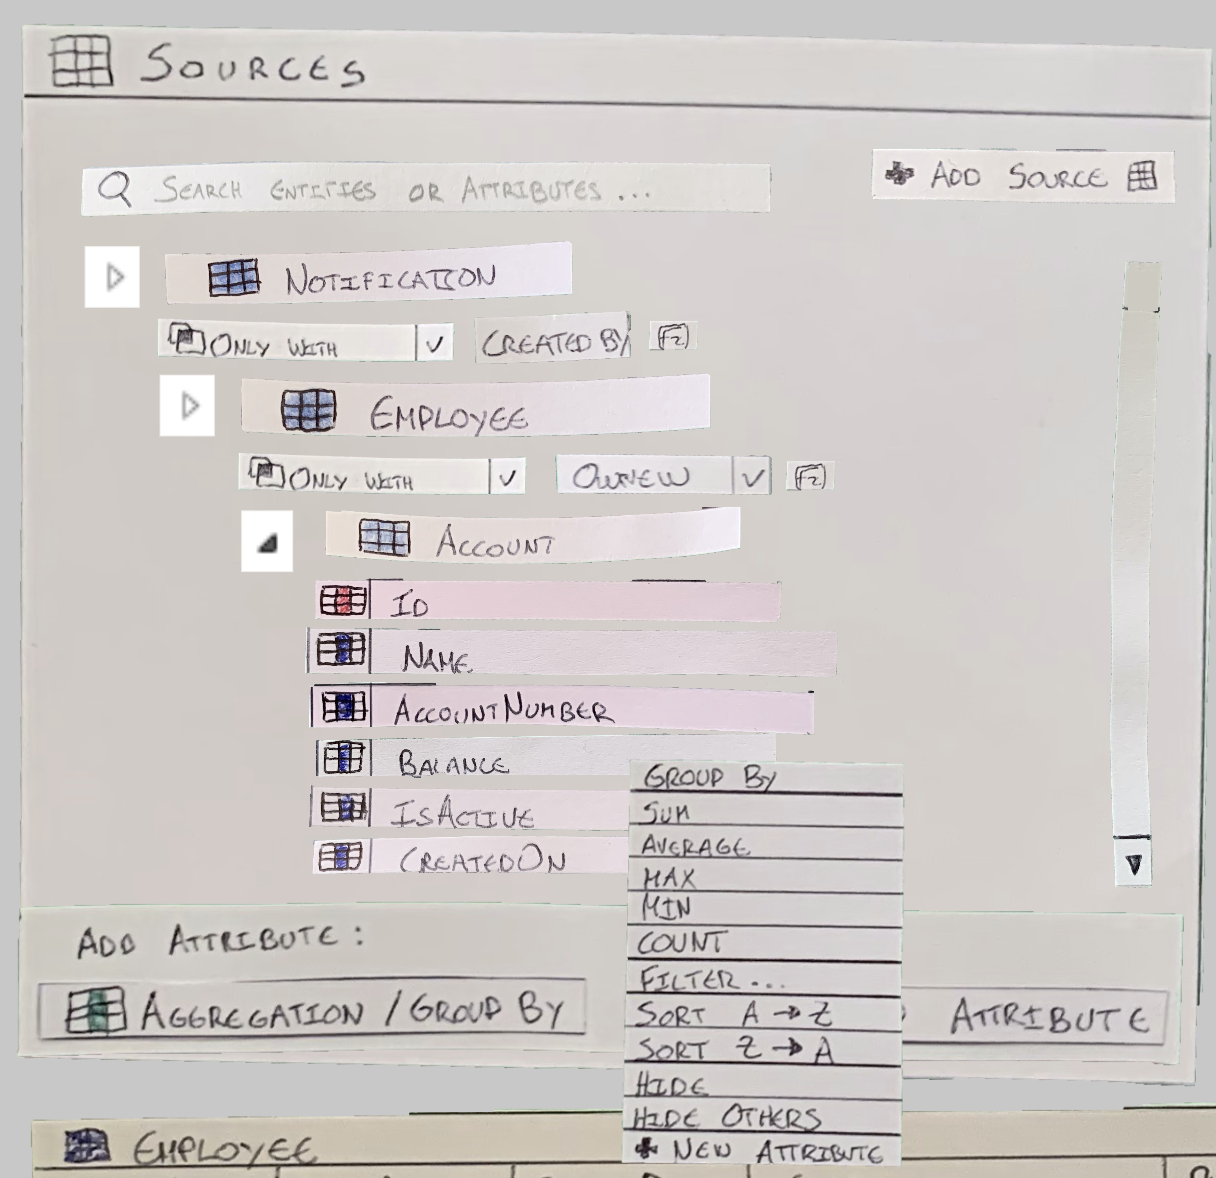
\includegraphics[height=2.4in]{paper-attribute-right-click}
	\caption{Alternative provided to open the attribute context menu.}
	\label{fig:paperAttributeRightClick}
\end{figure}

\begin{figure}[htbp]
	\centering
  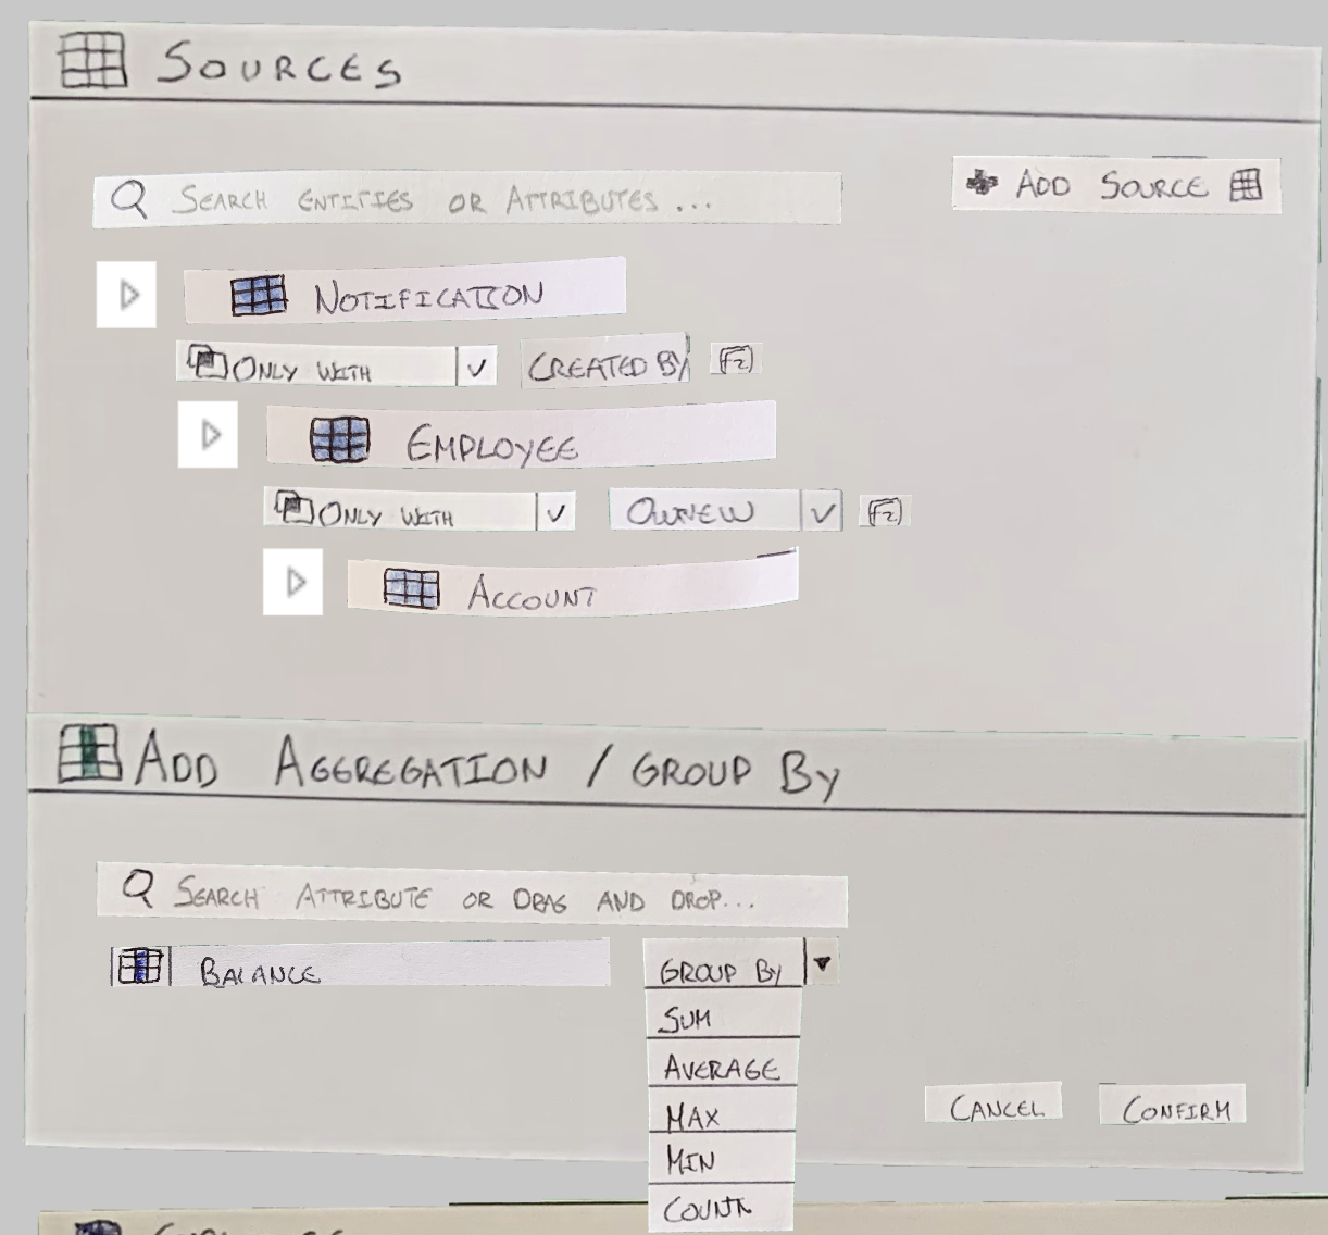
\includegraphics[height=2.4in]
  {paper-add-aggregation}
	\caption{New sub-editor into the sources view to add aggregation functions and group bys.}
	\label{fig:paperAddAggregation}
\end{figure}

\begin{figure}[htbp]
	\centering
  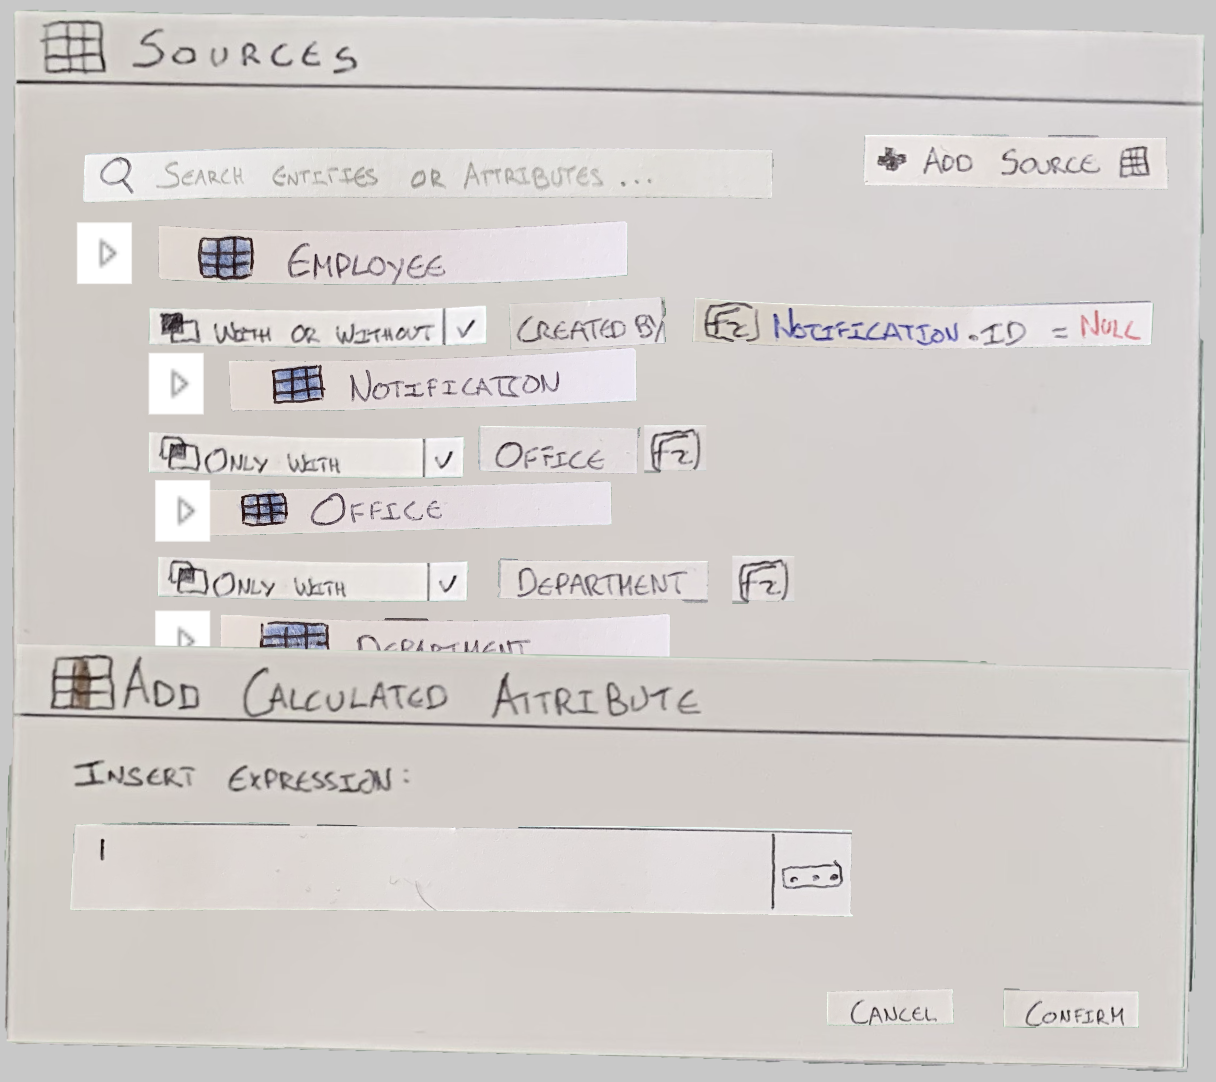
\includegraphics[height=2.4in]
  {paper-add-calculated-attribute}
	\caption{New sub-editor into the sources view to add calculated attributes.}
	\label{fig:paperAddCalculatedAttribute}
\end{figure}

In order to improve the query readability and the consistency of the interface, these attributes, added to the query, were put into the sources view as exemplified in Figure \ref{fig:paperAggregatedAttribute}.

\begin{figure}[htbp]
	\centering
  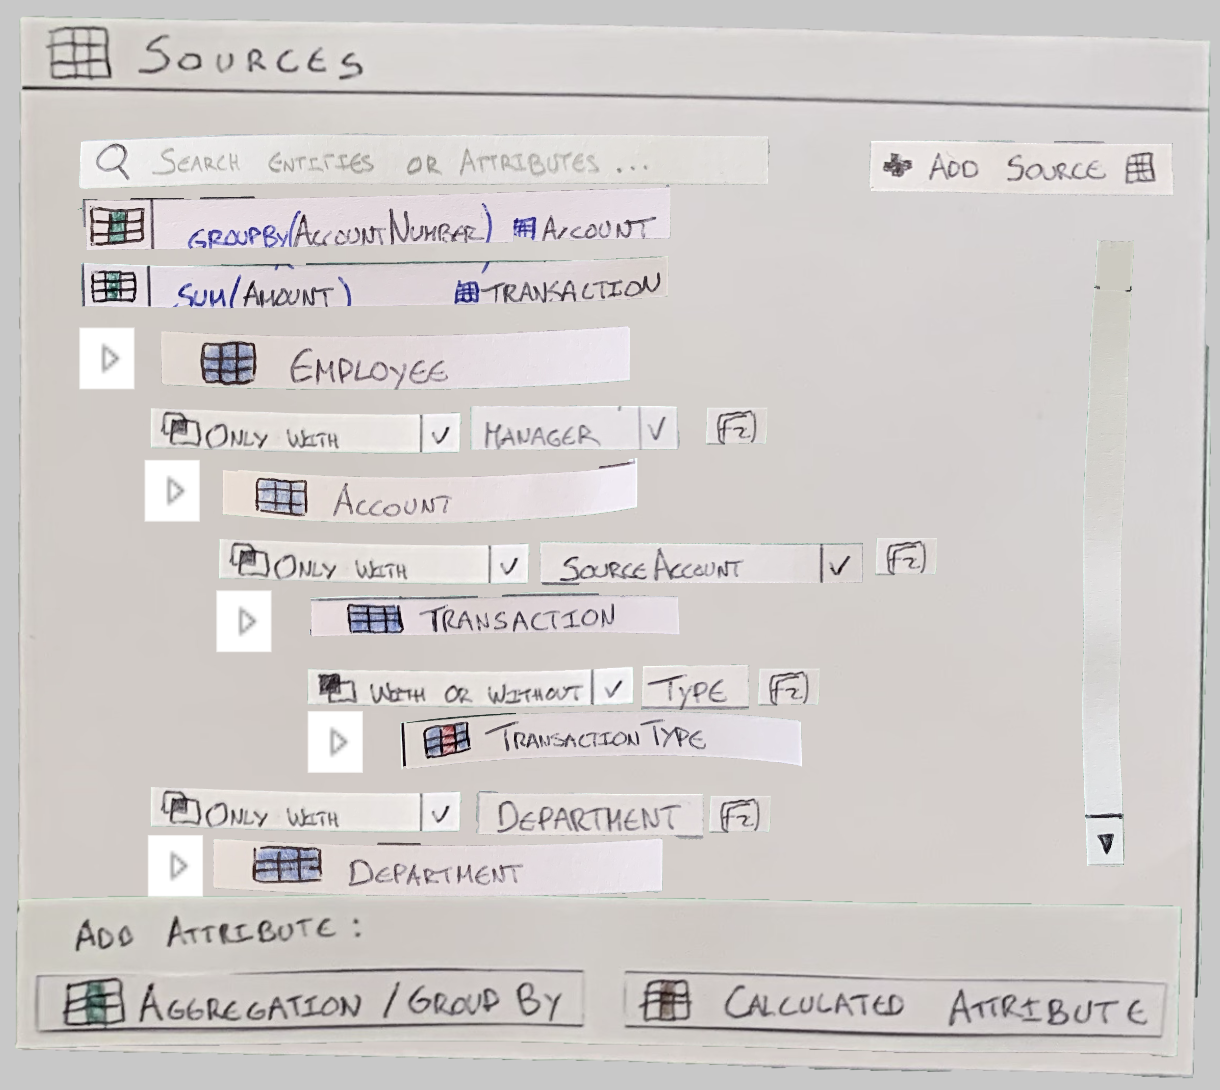
\includegraphics[height=2.4in]
  {paper-aggregated-attribute}
	\caption{Sources of a query where a group by and a SUM aggregation function were applied.}
	\label{fig:paperAggregatedAttribute}
\end{figure}

\medskip

\textbf{Digital Paper Prototype: }

\medskip

Combining all the components elaborated in paper, the result is illustrated in Figure \ref{fig:paperPrototypeExample}. In order to make it testable remotely, each one of the interface components were scanned and composed again using the InVision App \cite{invision}.

\begin{figure}[htbp]
	\centering
  \includegraphics[height=3.2in]
  {paper-prototype-example}
	\caption{Final Paper Prototype before scanning it.}
	\label{fig:paperPrototypeExample}
\end{figure}

Therefore, for each scenario, it was required to build multiple images since each one represents a state among the interface manipulation. In that way, interactions were added to the components to configure the images sequence, as can be observed in Figure \ref{fig:invisionInteractionExample}.

\begin{figure}[htbp]
	\centering
  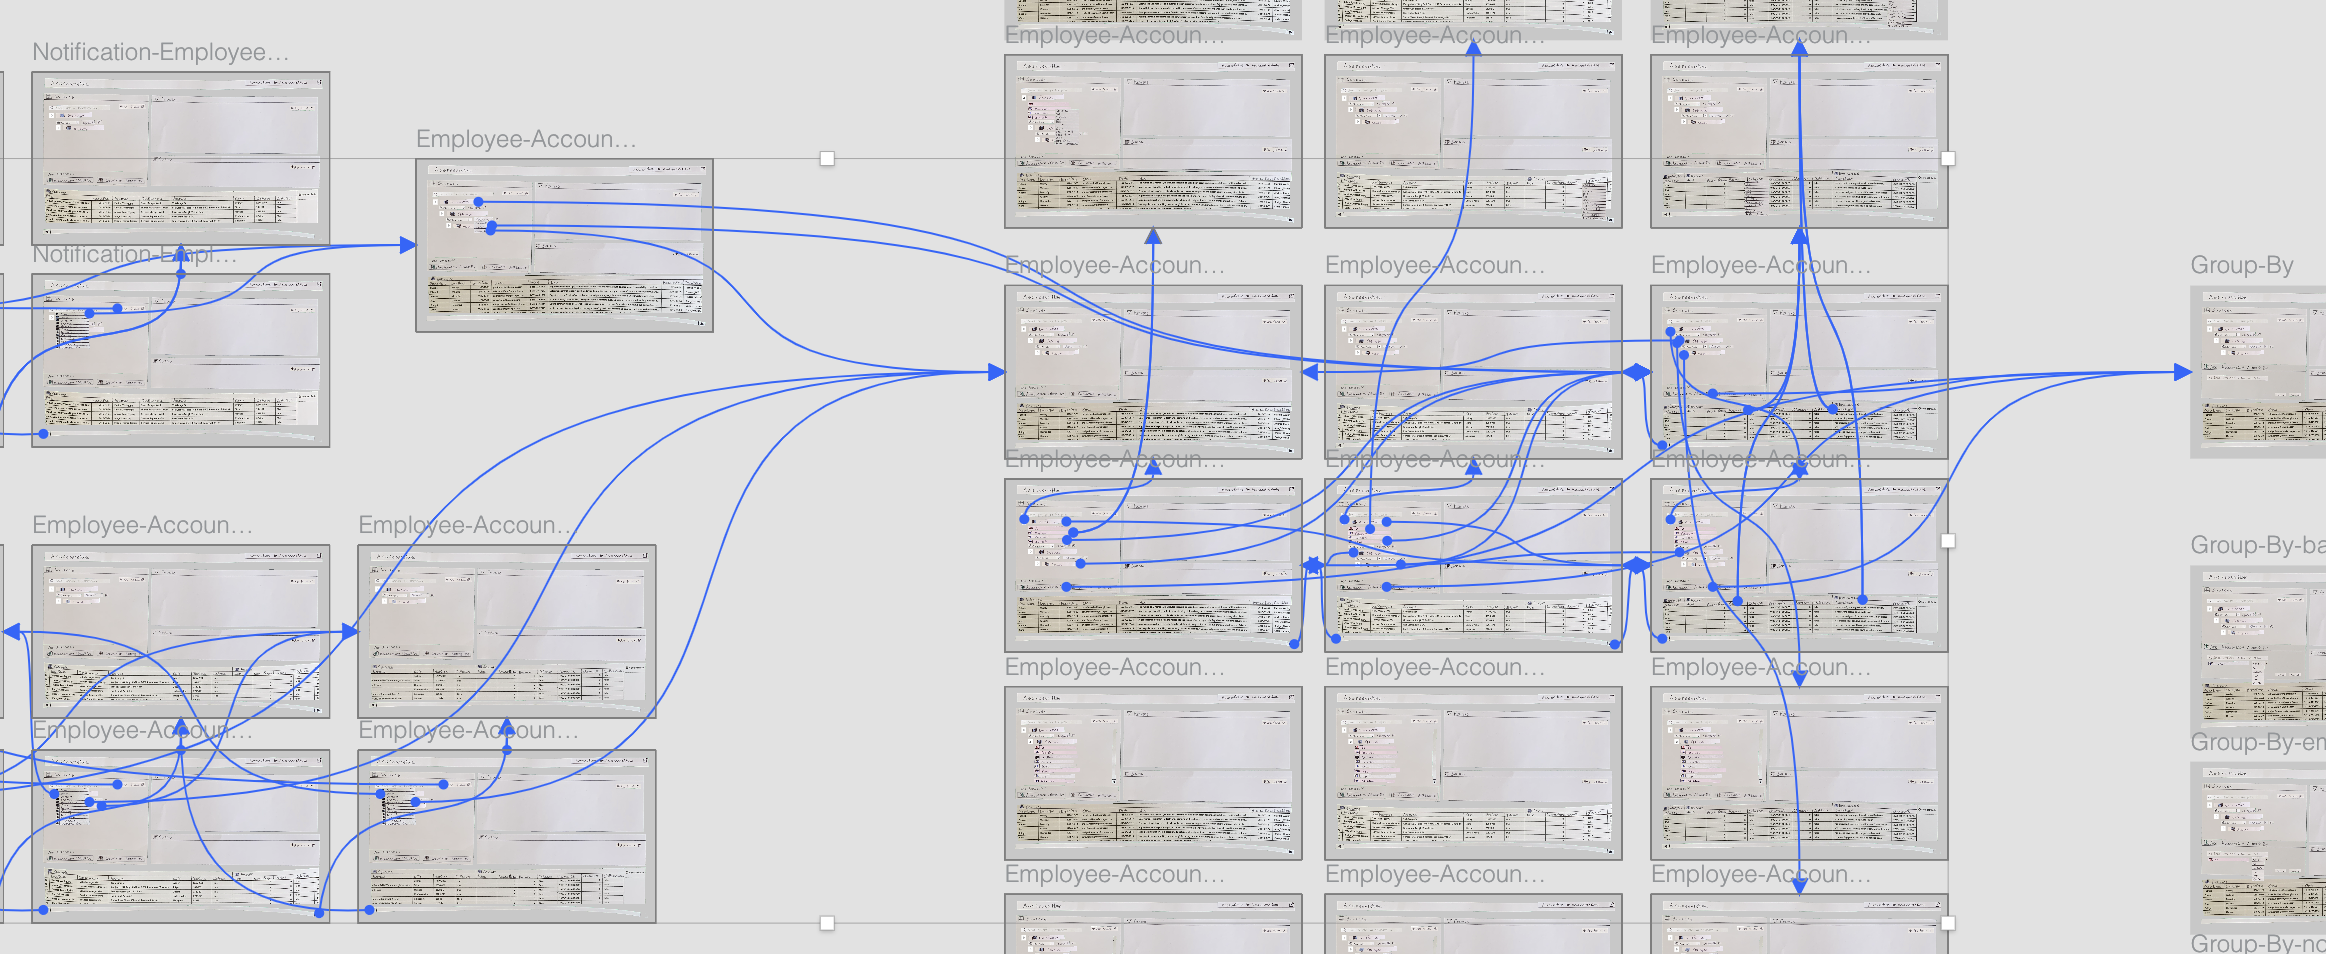
\includegraphics[height=2.4in]
  {invision-interaction-example}
	\caption{Brief example of the interaction configuration in InVision to turn the Paper Prototype testible in a fluid way.}
	\label{fig:invisionInteractionExample}
\end{figure}

In total, 291 images were created and, multiple interactions between them were configured, in order to reach a prototype that could be tested in all scenarios defined in the Appendix \ref{app:user_testing_scenarios} - \nameref{app:user_testing_scenarios} \cite{invision_managing_interactions}

%Tabela do resultado para cada scenario
%Filtros e sorting de cada scenario

%New sources design
%-Falar sobre as chaves estrangeiras e a simplificação dos joins
%-Novas formas the inserir atributos
%-Apresentar solução proposta

% It is important to refer the implementation complexity of the prototype in InVision due to the interface complexity.

\subsection{Evaluation}
\label{subsec:paper_prototype_evaluation}

After completing the implementation of the Paper Prototype, the user testing phase has started. As mentioned in \ref{sec:iterative_design}, this prototype was tested with 5 users of each user group to perform a qualitative analysis regarding the changes applied in the interface. The testing methodology used was the same used to test the existing interface evaluation, described in \ref{sec:existing_interface_evaluation}. Accordingly, the Zoom \cite{zoom} meeting solution was used to share and record the screen, showing the Paper Prototype built in InVision \cite{invision}, thus users managed to interact with the prototype using the Zoom remote control feature. In that way, the aim, at this stage, was to map the improved aspects and details which require a redesign in the following phase.

As a general result, by observing users using the interface, the new sub-editors layout applied was accepted positively by the users, even the ones who were more accustomed to the previous tab layout. Although, at a first glance, some users claimed feeling overloaded with information, they mentioned, that seeing all query structure in a short visualization area above was useful. Other feedback pointed out was that it could be useful to resize the dimensions of each sub-editor area.

Regarding the query result preview, some users did not manage to comprehend which attributes belong to the query output against the ones that were only a preview to understand the aggregations or group bys applied.\footnote{As mentioned in section \ref{subsubsec:current_progress} and exemplified in Figure \ref{fig:aggregations_example}, the query output preview not only presents the attributes that belong to the query output but also a preview of the data related to the aggregated attributes.} 
Even though it was difficult to distinguish the two elements of the query result, since it was used a low expressiveness in terms of color, this constraint will be taken into account in the next design iteration since more styling and color resources will be available.

As predicted in the design and implementation phases of this prototype, the completely redesigned sources editor triggered different points of view and interesting feedback for the next iteration design phase.

Therefore, the following points describe the information collected with respect to the users' comprehension of this new representation:

\begin{itemize}
  \item Some users misinterpreted the joins of some queries due to the indentation used to represent them. For instance, in the example shown in Figure \ref{fig:paperPrototypeExample}, some users indicated that "Office" was joined with "Department", when "Office" was joined with "Employee";
  \item Some users did not manage to understand what the foreign key label was, until they need to select one of them in the formulation scenario. That way, the representation of this element should be reevaluated to make it more clear. Nevertheless, the results concerning the identification of the foreign key, presented in Table \ref{tab:paperPrototypeForeignKeyIdentification}, are positive since considering all user groups 77.78\% of users have identified correctly the foreign key in the causes that entities could be joined using different attributes. Therefore, although the positive results, the lack of intuitiveness regarding the foreign key presentation perceived by users when they observed the interface at the first sight was considered as an aspect to improve in the following design iteration;
  \item Regarding the join conditions simplification, it was identified an increased awareness, when compared to the existing interface, to perceive that there were two representations of join conditions, as shown in Figure \ref{fig:paperComprehension1Sources}. The majority of users did not manage to understand the meaning of these different visual representations, which intended to differentiate joins automatically generated from the ones manually edited, as Table \ref{tab:paperPrototypeLeftJoinNull} points out since only 26.67\% of users have identified clearly the join purpose.
\end{itemize}

%TODO: Tables left join with foreign key identification, selection
%Conclude about results with comparing with the previous interface


% Please add the following required packages to your document preamble:
% \usepackage{booktabs}
\begin{table}[tb]
  \caption{Readability of the foreign keys used to join entities that could be joined using different attributes. (Paper Prototype usability tests - 15 users)}
    \label{tab:paperPrototypeForeignKeyIdentification}
  \begin{tabular}{@{}lrrr@{}}
  \toprule
  \textbf{Foreign Key Identification} & \multicolumn{1}{l}{Identified} & \multicolumn{1}{l}{Did not Identify} & \multicolumn{1}{l}{Did not see the Join} \\ \midrule
  OutSystems Developer                & 86.67\%                        & 13.33\%                              & 0.00\%                                   \\
  Software Developer                  & 66.67\%                        & 33.33\%                              & 0.00\%                                   \\
  Citizen Developer                   & 80.00\%                        & 20.00\%                              & 0.00\%                                   \\
  Total                               & 77.78\%                        & 22.22\%                              & 0.00\%                                   \\ \bottomrule
  \end{tabular}
  \end{table}

% Please add the following required packages to your document preamble:
% \usepackage{booktabs}
\begin{table}[tb]
  \caption{Readability rate of the join which represents the case where two entities were merged using a left join and the conditions specified the that the primary key of the right enitity must be null. (Paper Prototype usability tests - 15 users)}
    \label{tab:paperPrototypeLeftJoinNull}
  \begin{tabular}{@{}m{5.4cm}rrr@{}}
  \toprule
  \textbf{Left Join with Null Identifier Comprehension} & \multicolumn{1}{l}{Identified} & \multicolumn{1}{l}{Did not Identify} & \multicolumn{1}{l}{Did not see the Join} \\ \midrule
  OutSystems Developer                                  & 40.00\%                        & 60.00\%                              & 0.00\%                                   \\
  Software Developer                                    & 20.00\%                        & 80.00\%                              & 0.00\%                                   \\
  Citizen Developer                                     & 20.00\%                        & 80.00\%                              & 0.00\%                                   \\
  Total                                                 & 26.67\%                        & 73.33\%                              & 0.00\%                                   \\ \bottomrule
  \end{tabular}
  \end{table}


Furthermore, the following aspects were captured from observing users trying to formulate queries:

\begin{itemize}
  \item As expected, the foreign key selection method presented in Figure \ref{fig:paperFkSelect} has optimized the effectiveness of the formulation scenario. Since users were asked to choose between the existing foreign key, they were able to select the correct one. The results presented in Table \ref{tab:paperPrototypeForeignKeySelection} illustrates the effect of the improvement made in the interface since all users have selected the correct foreign key to indicate the properly join the formulation case that was necessary to add a join to merge two entities that could be joined using three different foreign keys;
  \item Concerning the two new buttons to add aggregation functions, group bys, and calculated attributes, it was concluded that, the results have enhanced, but some drawback aspects were identified. Users who have never used the system, found these features easy since the two buttons became visible in the interface. However, they continue to make misunderstand when they needed to use a calculated attribute or the aggregation function:
  \begin{itemize}
    \item Insert Calculated Attribute: The users' acceptance to the new options provided to insert calculated attributes was positive. Not only users who not have already used the query builder have less difficulty to create new attributes, since only 20\% of Software Developers and 40\% of Citizen Developers had difficulty to find the options and the remaining ones managed to added it intuitively, as detailed in Table \ref{tab:paperPrototypeCalculatedAttribute}, but also the new options provided were used by OutSystems Developers who are accustomed to use the previous query builder interface. As Table \ref{tab:paperPrototypeOptionCalculatedAttribute} demonstrates, the new button added on the bottom of the sources view was used by 86.67\% of users. Besides, even 80\% of the OutSystems Developers, who knew the existence of a button on the final of the query result table, preferred to use the new option to add the attribute, so that the acceptance of that changes was positive not only to mitigate learnabilty problems of users who had not found the option before in the existing interface, but also for expert users that preferred this option more accessible.
  \end{itemize}
\end{itemize}

% Please add the following required packages to your document preamble:
% \usepackage{booktabs}
\begin{table}[tb]
  \caption{Selection of the foreign key, in the formulation scenario, used to join entities that could be joined using different attributes. (Paper Prototype usability tests - 15 users)}
  \label{tab:paperPrototypeForeignKeySelection}
  \begin{tabular}{@{}lrrr@{}}
  \toprule
  \textbf{Foreign Key Selection} & \multicolumn{1}{l}{Selected} & \multicolumn{1}{l}{Did not Select} & \multicolumn{1}{l}{Did not Add the Join} \\ \midrule
  OutSystems Developer           & 100.00\%                     & 0.00\%                             & 0.00\%                                   \\
  Software Developer             & 100.00\%                     & 0.00\%                             & 0.00\%                                   \\
  Citizen Developer              & 100.00\%                     & 0.00\%                             & 0.00\%                                   \\
  Total                          & 100.00\%                     & 0.00\%                             & 0.00\%                                   \\ \bottomrule
  \end{tabular}
  \end{table}

% Please add the following required packages to your document preamble:
% \usepackage{booktabs}
\begin{table}[tb]
  \caption{Success rate of users when they needed to add a calculated attribute. (Paper Prototype usability tests - 15 users)}
  \label{tab:paperPrototypeCalculatedAttribute}
  \begin{tabular}{@{}m{5cm}rrr@{}}
  \toprule
  \textbf{Insert Calculated Attribute} & \multicolumn{1}{l}{Added Successfully} & \multicolumn{1}{l}{Difficulty to Add} & \multicolumn{1}{l}{Could not Add} \\ \midrule
  OutSystems Developer                 & 100.00\%                               & 0.00\%                                & 0.00\%                            \\
  Software Developer                   & 80.00\%                                & 20.00\%                               & 0.00\%                            \\
  Citizen Developer                    & 60.00\%                                & 40.00\%                               & 0.00\%                            \\
  Total                                & 80.00\%                                & 20.00\%                               & 0.00\%                            \\ \bottomrule
  \end{tabular}
  \end{table}


% Please add the following required packages to your document preamble:
% \usepackage{booktabs}
\begin{table}[tb]
  \caption{Options used by users to insert the calculated attribute in the context of the M1 scenario. (Paper Prototype usability tests - 15 users)}
  \label{tab:paperPrototypeOptionCalculatedAttribute}
  \begin{tabular}{@{}m{4.4cm}R{3.1cm}R{3.1cm}R{3.1cm}@{}}
  \toprule
  \textbf{Option used to insert the calculated attribute} & \multicolumn{1}{m{3.1cm}}{Add button on the bottom of the Sources View} & \multicolumn{1}{m{3.1cm}}{Right click in the attributes tree (Sources View)} & \multicolumn{1}{m{3.1cm}}{Add button on the result table (after all attributes)} \\ \midrule
  OutSystems Developer                                    & 80.00\%                                                          & 0.00\%                                                                & 20.00\%                                                                   \\
  Software Developer                                      & 100.00\%                                                         & 0.00\%                                                                & 0.00\%                                                                    \\
  Citizen Developer                                       & 80.00\%                                                          & 20.00\%                                                               & 0.00\%                                                                    \\
  Total                                                   & 86.67\%                                                          & 6.67\%                                                                & 6.67\%                                                                    \\ \bottomrule
  \end{tabular}
  \end{table}

Finally, some users referred that they felt a reduced necessity to confer the Data Model while they were building queries, since the new sources representation shown how entities were related with each other

In conclusion, the general success results of the 15 users performing the scenarios proposed, presented in Table \ref{tab:effectiveness_paper_prototype}, were positive although the improvement topics already stated. Therefore, the design implemented in the paper prototype was considerable favourable to optimize the usability of the interface for the different user groups analyzed. In that way, the following prototyping iteration will take into account the feedback users provided in this evaluation stage as well as the results obtained.


%Comparison with Existing Interface Evaluation

%Quantos utilizadores foram testados
%Dada a população utilizada só foram feitas análises qualitativas como meio de obter feedback construtivo para a próxima iteração.

%Explicar resultados mais importantes
%-Verificar os outros resultados
%-Melhoria da sources view visto que os utilizadores não perceberam que se tratava da chave estrangeira.
%Para além disso houve quem não achasse clara a apresentação devida à identação utilizada. (Por exemplo confundiram que tabela se relaciona com qual. Utilizar o exemplo do Comprehension 1 para justificar)

%-No geral o problema da leitura do left join com null manteve-se

%-Confundiram quando é que devia ser adicionado um calculated attribute e uma aggregation function.

%V-Alguns utilizadores referiram que o tamanho dos sub editores devia ser resizable

%-Divide add aggregation / group by into two different buttons

%-Some users said that the sources view is confusing at the first place but after some scenarios when he said that is easy.

%-Deveria ser apresentada uma maior distinção entre os atributos que estão no output e aqueles que não estão.

%-Tentaram expandir a source para adicionar joins.

%-Houve quem referisse que com esta interface existiu menos necessidade de observar o data  model

\section{Service Studio Implementation}
\label{sec:service_studio_implementation}

As mentioned in \ref{subsec:visual_development_environment}, Service Studio is the \gls{IDE} integrated in the OutSystems Platform that allows users to build full applications using the low-code programming paradigm. In that way, the last iteration of the design process, and consequently, the final prototype elaborated in this dissertation, was a functional prototype of the query builder completely integrated into the code of the Service Studio.

Nevertheless, Service Studio was getting a major facelift to achieve a new revamped and refreshed design. Even though the new Service Studio design has not been released yet, the development of the final prototype was decided to be done using the new Service Studio look. In that way, the interface of the query builder developed could be easily integrated later on the OutSystems Platform. Figure \ref{fig:aggregateNewDesign} illustrates the design used as the starting point for the final prototype development. As can be observed, is a redesigned version of the previous Service Studio design illustrated before in Figures \ref{fig:ss_workspace} and \ref{fig:aggregate_created}

\begin{figure}[htbp]
	\centering
  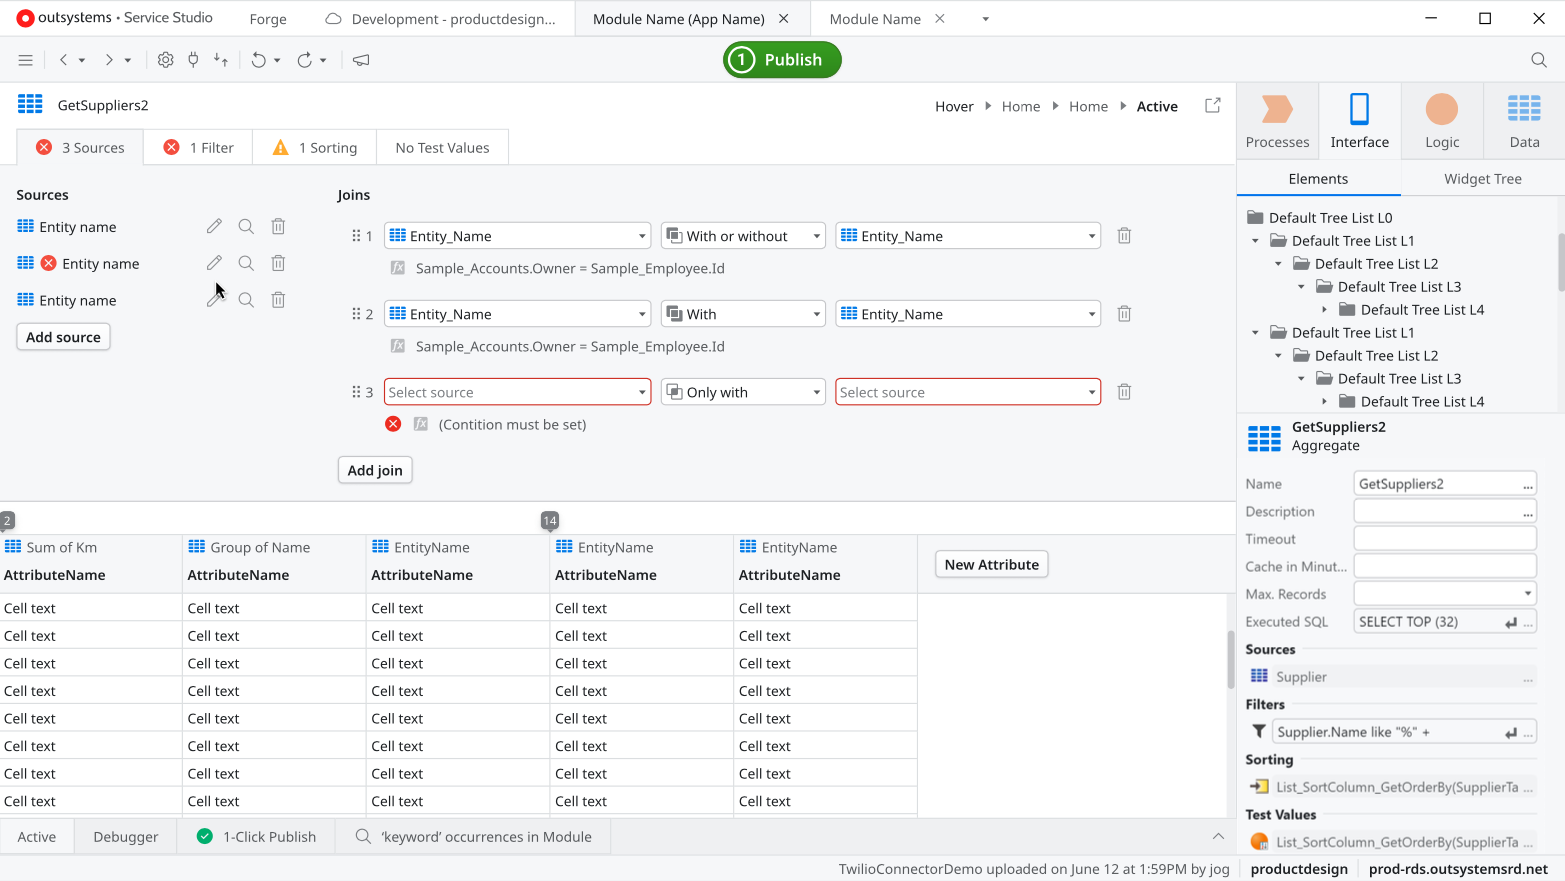
\includegraphics[height=3.0in]
  {aggregate-new-design-2}
	\caption{The new design of the Service Studio and its Visual Query Builder.}
	\label{fig:aggregateNewDesign}
\end{figure}

Despite the new design of all interface elements and components, the core behaviors and interactions of the interface remained, so the same design and implementation intentions to be applied in this new phase of development were maintained.

\subsection{Design}
\label{subsec:service_studio_design}

Following the same methodology used in the Paper Prototype, the building process of this solution started with the design phase. In this phase, the paper prototype evaluation outcomes were deliberated in order to define and prioritize the aspects to be tackled in the final prototype.

First of all, the source code of the Service Studio was explored in order to plan the development that could be done in the available time. As explained in the presentation of the paper prototype, the development aspects were planned according to their impact on the final interface. Ideas that fundamentally alter the experience of using the interface will be considered a priority, since, is primarily important to perceive how users react to those changes when testing the interface. Minor features and enhancements could also be considered as future work if the new interface solution evaluation show positive results.

Taking into account the evaluation of the Paper Prototype, the sources editor was considered the main focus of the design phase of the Final Prototype. As referred, during the usability tests of the paper prototype, the sources view has revealed positive results, but it was concluded that it should be refined regarding some aspects, mainly the joins representation which were not completely clear for a set of users.

Nevertheless, in order to implement the new interface representation of entities and joins, a considerable implementation effort would be required. The visualization area requires a personalized hierarchical view that should be built from scratch, since there is no similar element in the rest of the Service Studio.

Accordingly, before implementing any idea, a robust design should be established in order to avoid wasting implementation time on doing and redoing ideas. Therefore, it was performed more designs, regarding the sources editor of the interface, using the product design system components. Basically, it was used the Figma \ cite {figma}, which is a design tool where all the new Service Studio components were designed, to explore concrete options to represent sources and solve the problems found when users tested the Paper Prototype. By this means, it was possible to obtain a high-fidelity design faster and perceive what solution could most fit the existing requirements.

After exploring multiple alternatives, the options illustrated in Figure \ref{fig:sourcesFigma} were considered the most valuable. The main difference between them is the way joins are represented. In \nameref{fig:sourcesFigmaA}, the join is represented in a single line placed between the two entities involved. In \nameref{fig:sourcesFigmaB}, the join condition is represented after the the second entity involved in the join. Lastly, in \nameref{fig:sourcesFigmaC}, the second entity is presented on the right of the join kind.

\begin{figure}[tb]
  \centering
  \subcaptionbox{Option A\label{fig:sourcesFigmaA}}%
    {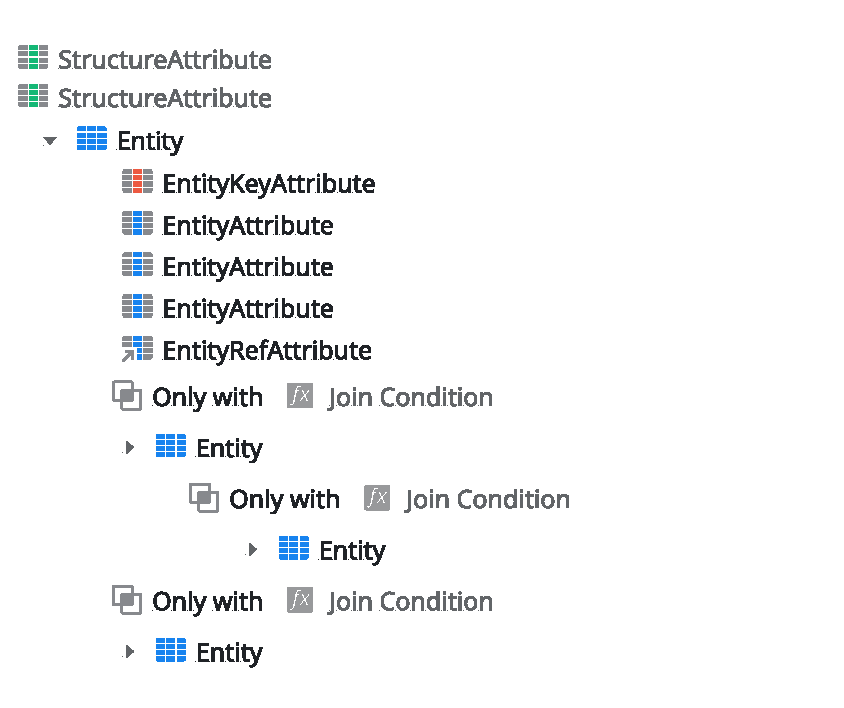
\includegraphics[height=2.5in]{sources-figma-1}}%
  \subcaptionbox{Option B\label{fig:sourcesFigmaB}}%
    {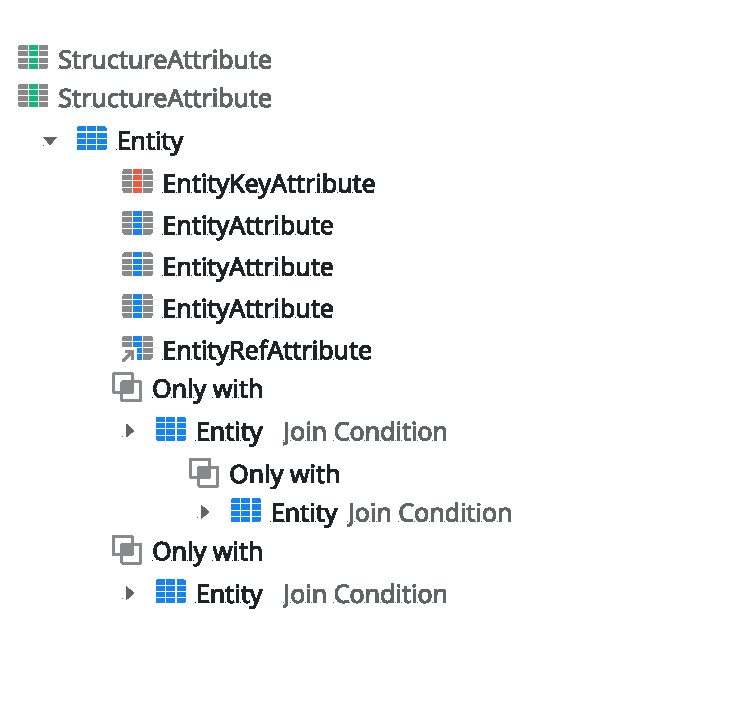
\includegraphics[height=2.5in]{sources-figma-2}}%
    \\
  \subcaptionbox{Option C\label{fig:sourcesFigmaC}}%
  {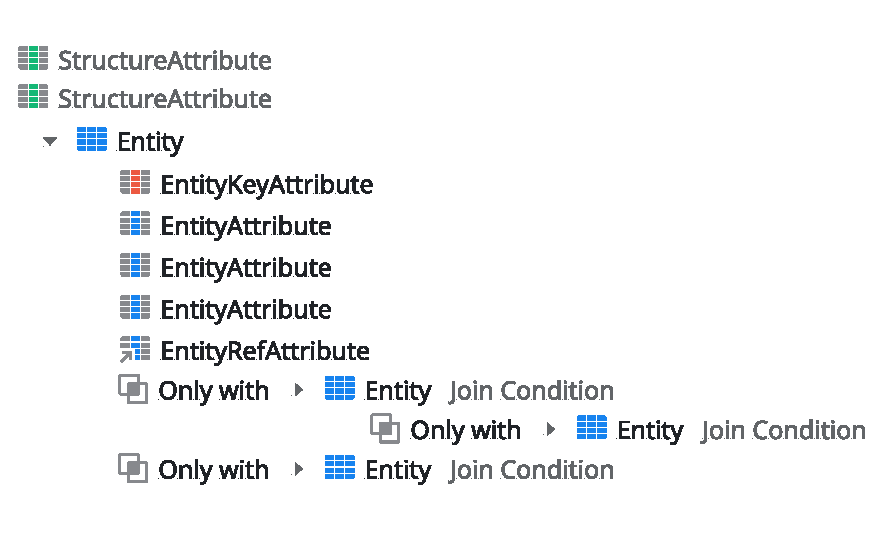
\includegraphics[width=0.5\linewidth]{sources-figma-3}}%
\caption{High-fidelity design ideas built in Figma to present the sources of the query.}
  \label{fig:sourcesFigma}
\end{figure}

In order to decide an option, the following topics were taken into account:

\begin{itemize}
  \item \textbf{Reading flow: } The flow of the entities and joins was considered important, especially due to the representation of the join kind. As this was presented in natural language, users should manage to read sequentially, first the entity, than the join, and after the second entity, all in a fluid way. Due to the arrangement adopted, the \nameref{fig:sourcesFigmaC} was considered the most clear regarding this aspect since the second entity is placed in the right side of the join kind. In that way, the users reading affordance will unconsciously help them to understand the reading flow, since becomes more natural due to the similarities with natural languages;
  \item \textbf{Width and height required: }The space that each option would occupy was important to analyze for the accommodation in the interface. Comparing the options presented, it can be concluded that the \nameref{fig:sourcesFigmaA} and \nameref{sub@fig:sourcesFigmaB} would require more height, and the \nameref{fig:sourcesFigmaC} more width;
  \item \textbf{Emphasis: }The used representation may end up giving more prominence to certain elements even though they were not built for that purpose. Accordingly, it was verified the aspects of the interface which would stand out at a first glance. In \nameref{sub@fig:sourcesFigmaA} and \nameref{sub@fig:sourcesFigmaB}, joins are more highlighted since there are specific lines to represent them. Conversely, in the \nameref{sub@fig:sourcesFigmaC} the join is presented in the same line of an entity, which makes entities standed out, in general. Therefore, the \nameref{sub@fig:sourcesFigmaC} was considered the most appropriated to highlight entities at a first sight.
\end{itemize}

Reflecting on the topics presented, the evaluation of the advantages and disadvantages of each option was conducted, the \nameref{fig:sourcesFigmaC} was elected, as preferred, since it provides a clear readability and highlights the entities used in the query. Despite it requires more width space in the interface, mainly if there are multiple joins nested, these disadvantages could be mitigated in the future if the join conditions would be simplified or represented in a different way.

Regarding the remaining elements of the interface, the design approaches applied in the Paper Prototype improved the usability of the interface. As a result, the design concerning filters, sorting and the query result table have followed the ideas already detailed in \ref{sec:paper_prototype}.


\subsection{Implementation}
\label{subsec:service_studio_implementation}
Bearing in mind the ideas explored in the paper prototype, and taking in account the evaluation performed with users, as well as, the high-fidelity design ideas built in Figma, the system started to be implemented in React \cite{react}, Typescript \cite{typescript} and C\#.

\medskip


\textbf{General layout:}

\medskip

Following the methodology used in the previous prototype, the first stage of the development process was to switch the tabs by an equivalent edition area with the three components visible at once (sources, filters, and sorting), as can be observed in Figure \ref{fig:withoutTabs}. Also, the existing scroll problem identified, illustrated in Figure \ref{fig:horizontalScrollBug}, (i.e., when users wanted to scroll the table horizontally to see the columns in overflow, the edition area above disappears) was solved. As a result, they are able to see all the components of the edition area and the information in the query result table at the same time. This change was important to reduce the users' working memory overload since they have the information they need visible.

%figure scroll problem

\begin{figure}[htbp]
	\centering
  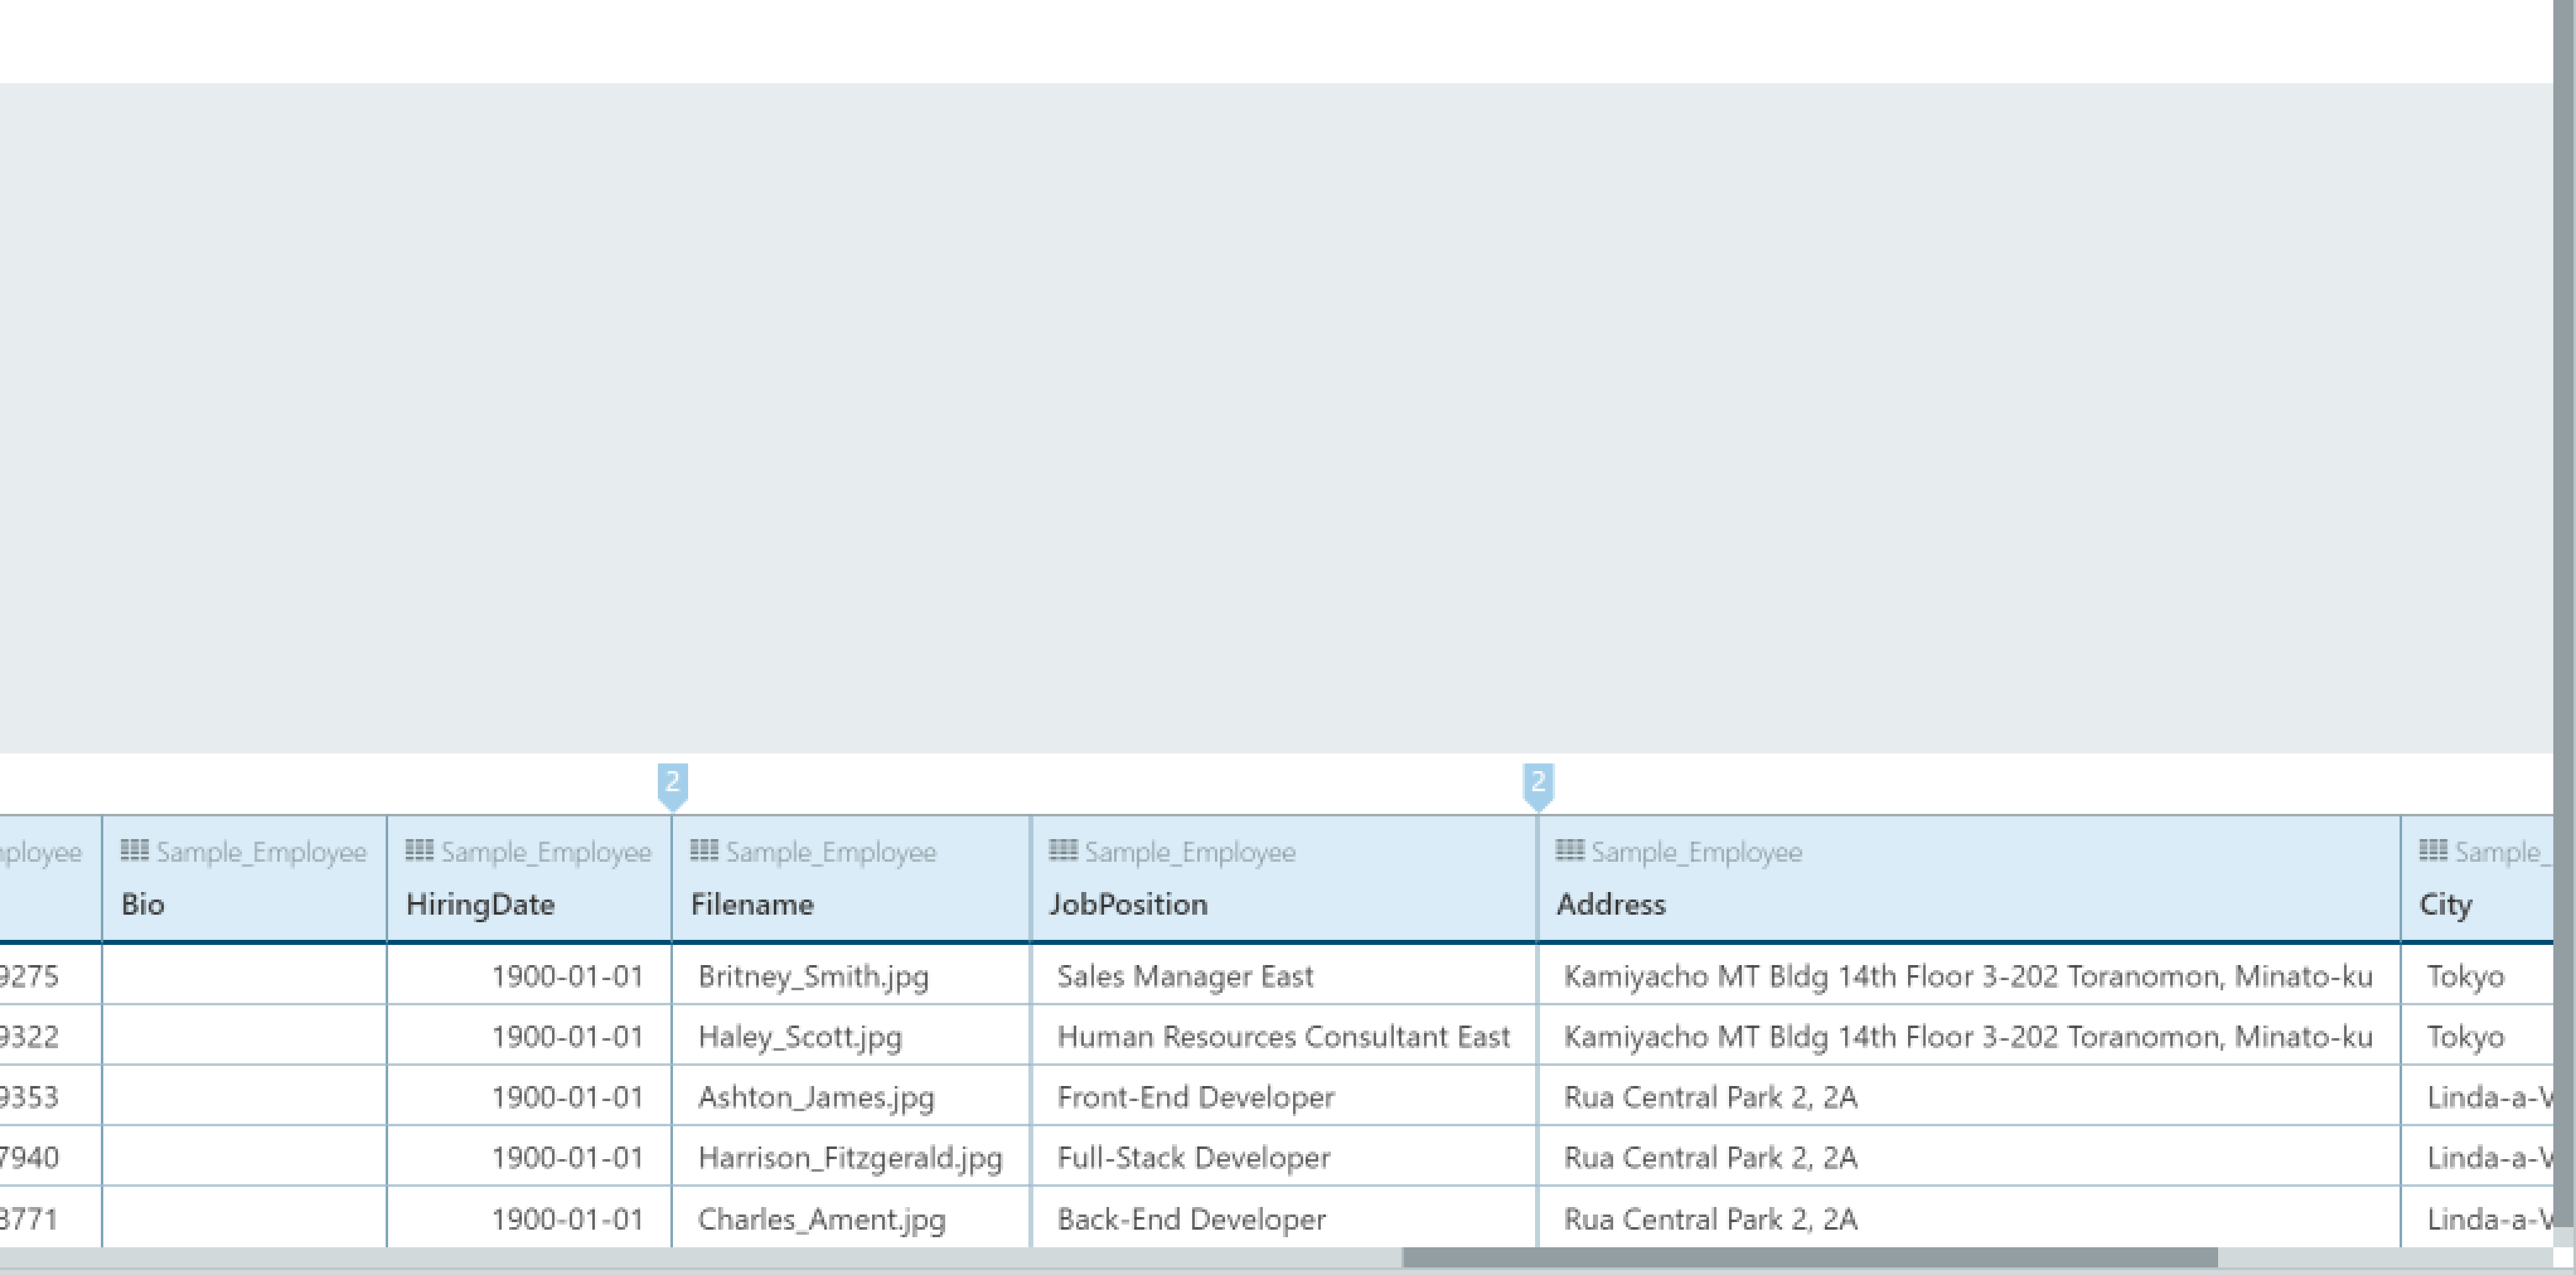
\includegraphics[height=2.0in]
  {horizontal-scroll-bug}
	\caption{Horizontal scroll problem in the existing interface: when users use scroll the see the columns at the right side, the editors are not fixed above.}
	\label{fig:horizontalScrollBug}
\end{figure}

%figure new sections (edit in figma to be easier)

\begin{figure}[htbp]
	\centering
  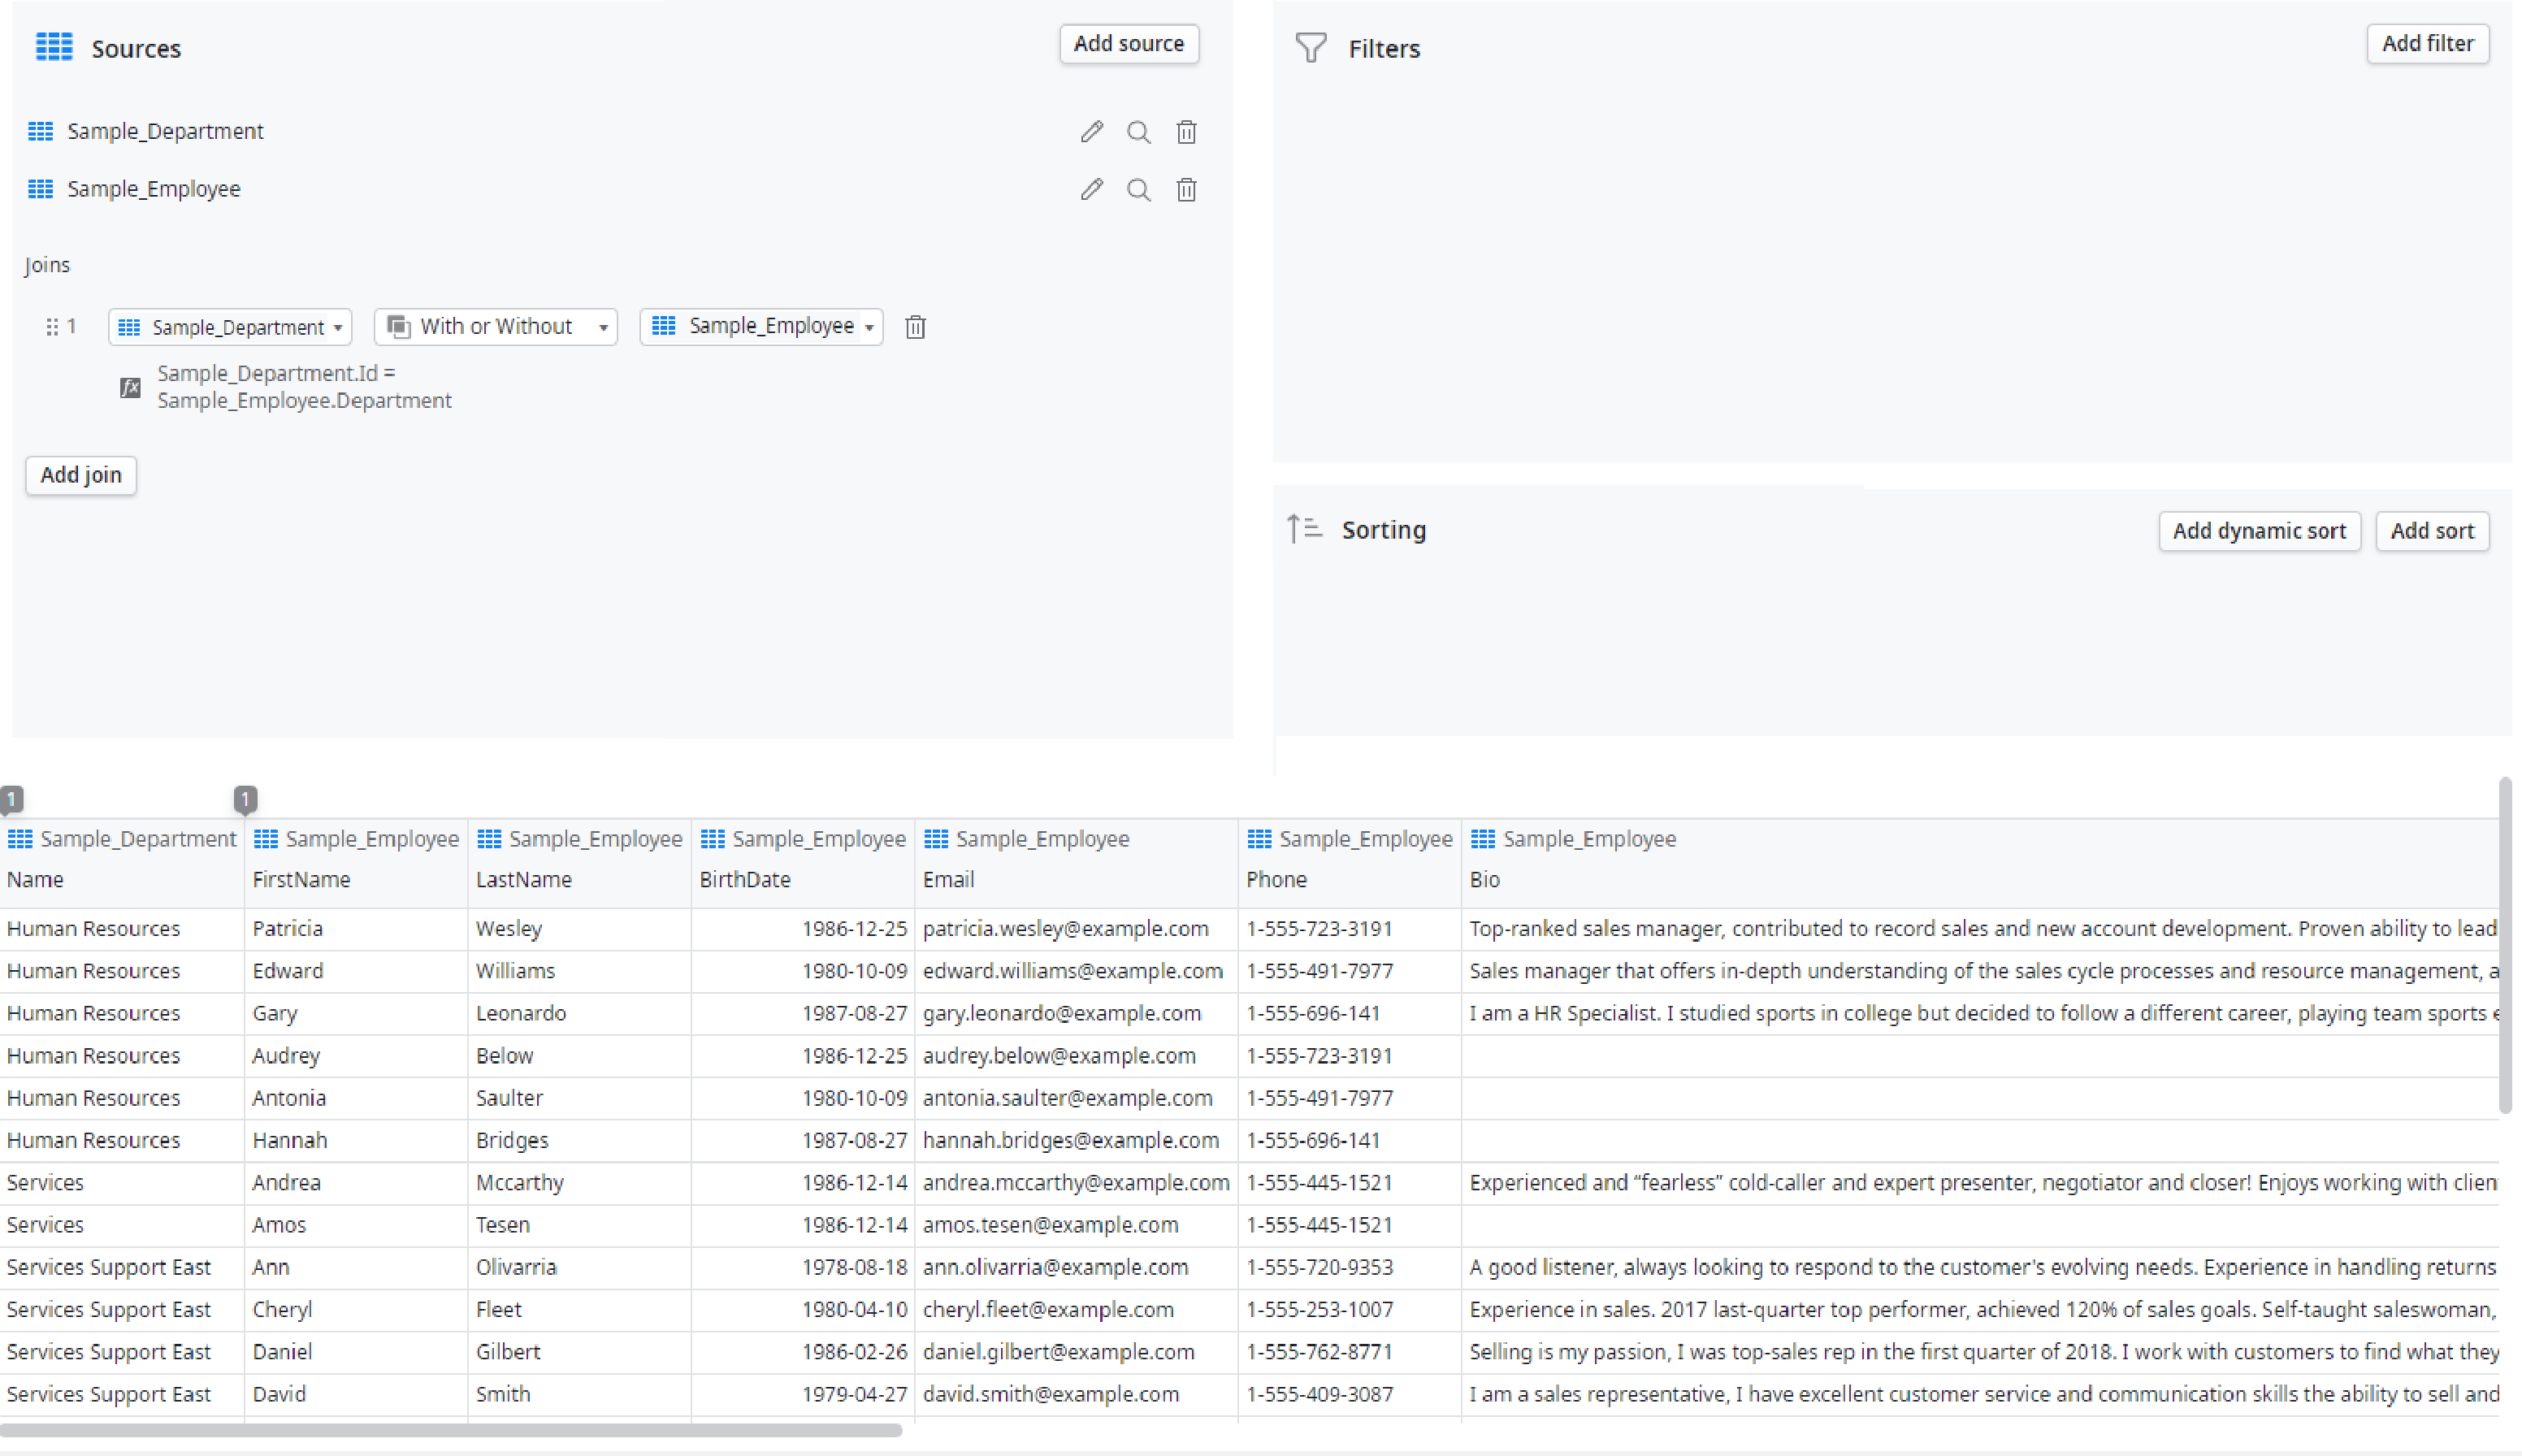
\includegraphics[height=2.8in]
  {without-tabs}
	\caption{Interface after removed the tabs and expanded them in three areas visible at the same time.}
	\label{fig:withoutTabs}
\end{figure}

\medskip

\textbf{Sources View:}

\medskip

As approached in the section above, the sources and joins editor has been completely redesigned. Since the design elaborated for this interface area presents multiple components using some indentation and nesting, the React components were structured before the implementation, they were organized, as shown in Figure \ref{fig:sourcesComponentsStructure}, in order to guarantee the feasibility of the arrangement created.

\begin{figure}[htbp]
	\centering
  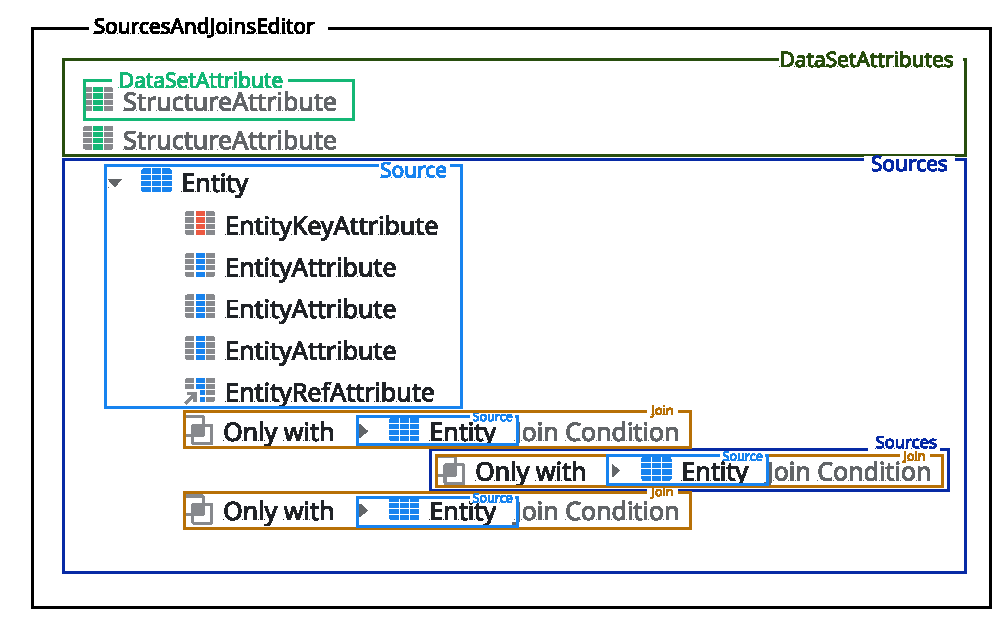
\includegraphics[height=3.0in]
  {sources-components-structure}
	\caption{Structure of the React components created to dispose the sources.}
	\label{fig:sourcesComponentsStructure}
\end{figure}

The $"SourcesAndJoinsEditor"$ is the parent component that contains all query sources. This component includes two areas: a list of  $"DataSetAttribute"$, which are the attributes of the query result added throughout the query formulation, such as aggregated attributes, group bys, or calculated attributes, and a component $"Sources"$ that represents all entities and joins of the query.

As the presentation of the entities and joins depends on the joins and the entities involved in the query, due to the indentation and nesting applied whenever an entity is joined with another already presented above, it was necessary to create some logic in the $"Sources"$ component to present the entities with the design intended.

Therefore, the $"Sources"$ renders the first entity added to the query, and after that, it iterates along the joins of the query to represent the ones that are related to the entity already rendered. For each join related to an entity, it is presented the join specification (i.e. join kind and join condition), however when the join is being generated, it is verifies if the entity joined to the previous one is related to more entities. In those cases, other $"Sources"$ is rendered to represent the remaining sources. Figure \ref{fig:withoutJoinSimplification} exemplifies the result of the interface implemented at this stage.


\begin{figure}[htbp]
	\centering
  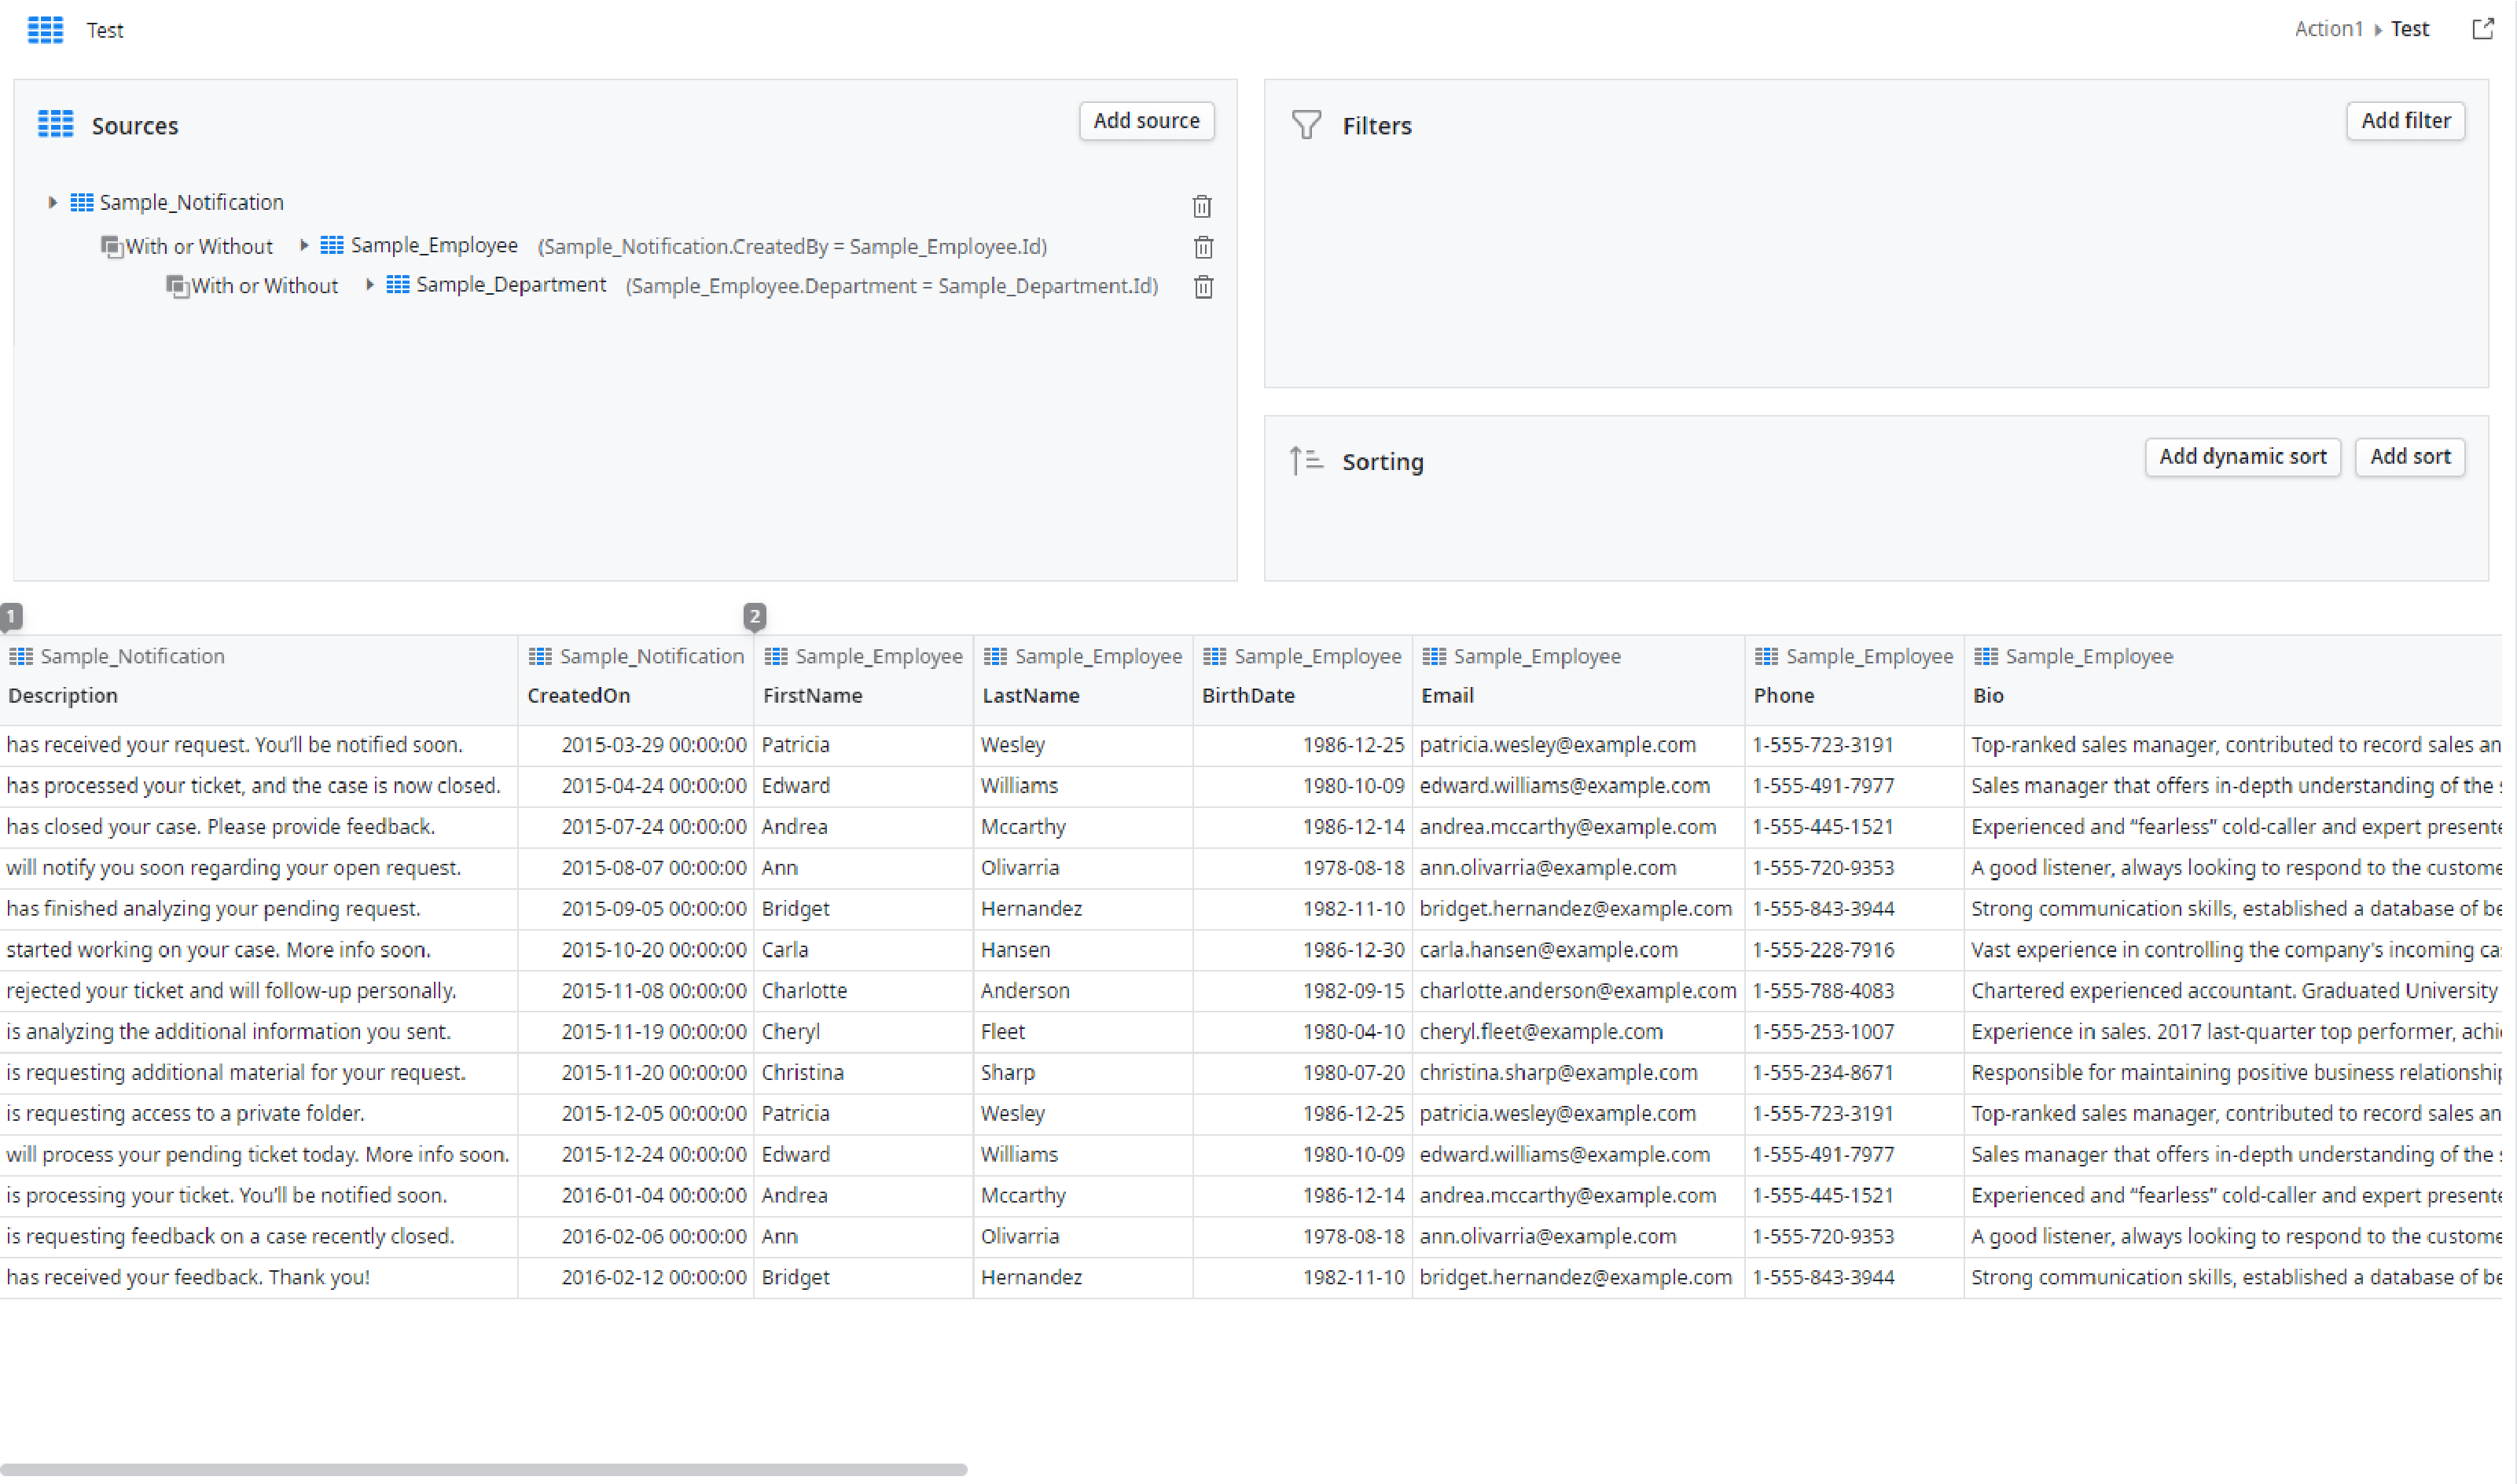
\includegraphics[height=3.0in]
  {without-join-simplification}
	\caption{Structure of the React components created to dispose the sources.}
	\label{fig:withoutJoinSimplification}
\end{figure}

Nevertheless, as referred in \ref{subsec:paper_prototype_implementation}, the join conditions which were generated automatically by the system were simplified. In those cases, the join conditions, on the existing interface, presented the primary key of an entity equal to a foreign key of the other entity, however since the characteristics of this formulation shown drawbacks for the users fully comprehension, it was designed a simplified version of the join condition. In this simplified version, only the foreign key is presented. If the join between the two entities could be made through different foreign keys, the foreign key used is presented in a dropdown, which allows users to change to another key if they intend. An example of a query with these dropdowns is presented in Figure \ref{fig:changeForeignKeyDropdown}. Through that approach, users not only can change that query aspect faster but also the data model could be perceived without consulting it directly, since the dropdown is an indicator that there are multiple attributes that could be used to join the two entities.

\begin{figure}[htbp]
	\centering
  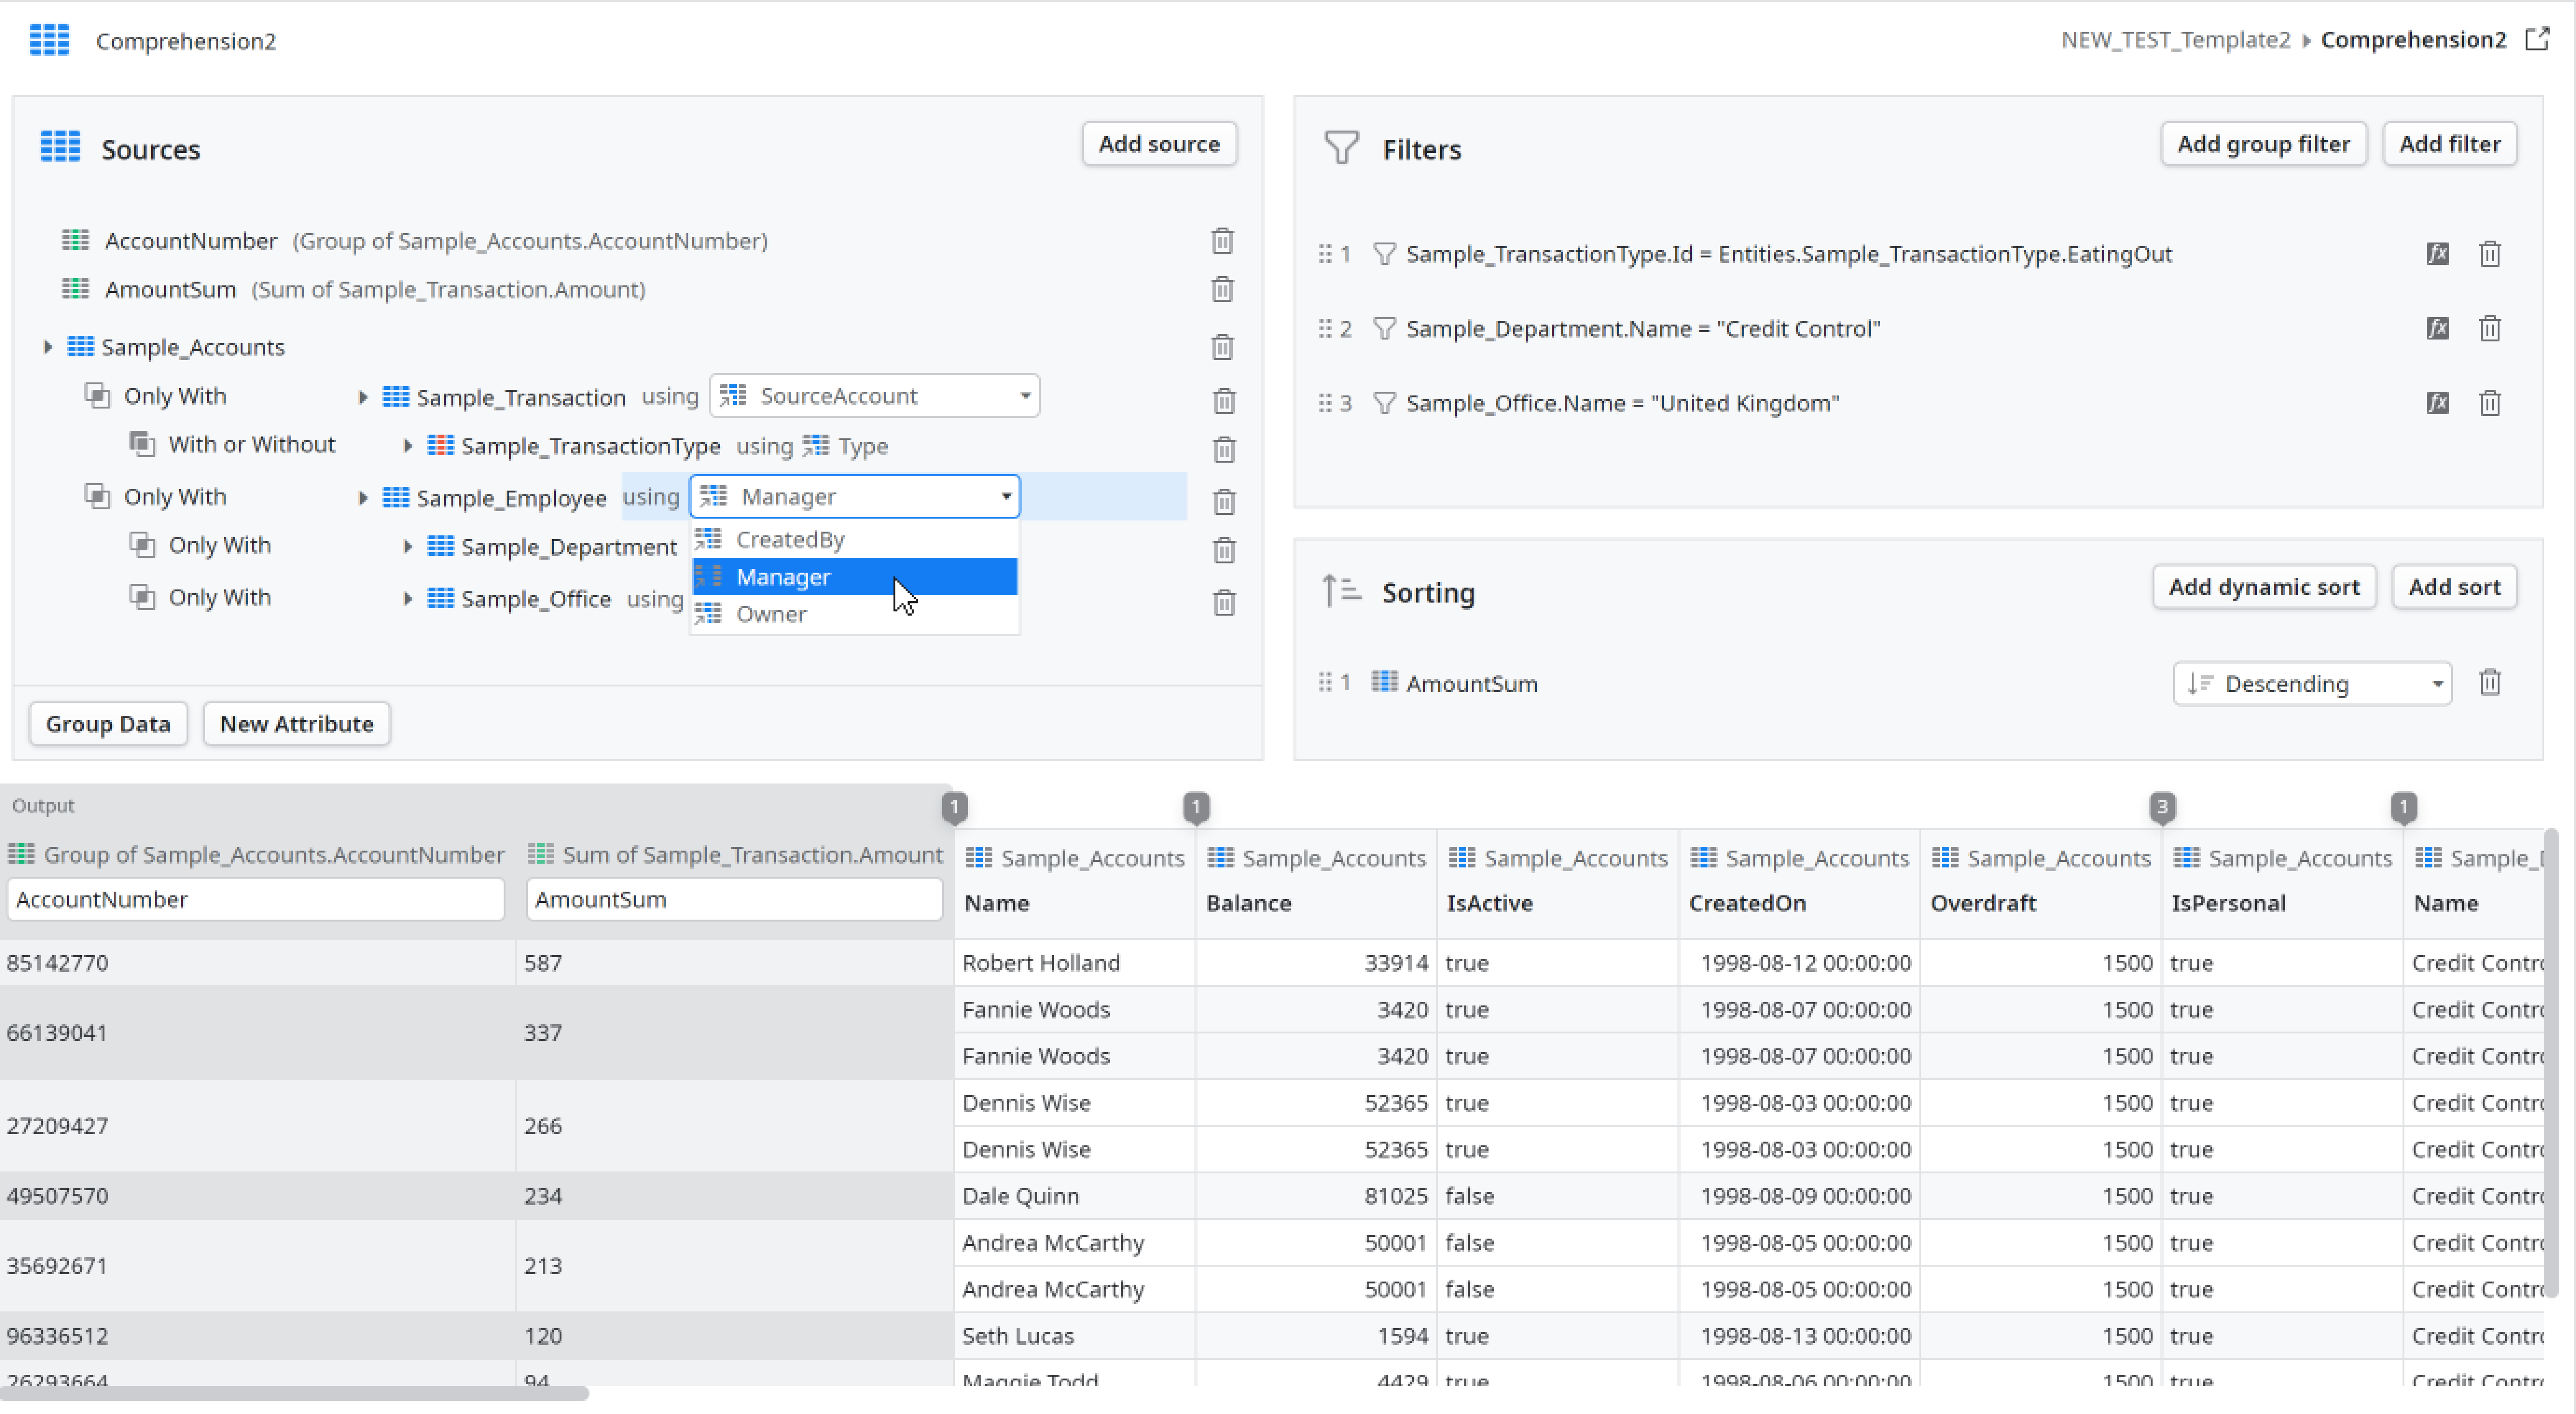
\includegraphics[height=3.0in]
  {change-foreign-key-dropdown}
	\caption{Example of a query were there are joins that could be applied using different foreign keys to merge the two entities, so the user can use the dropdown to choose the intended one.}
	\label{fig:changeForeignKeyDropdown}
\end{figure}

Furthermore, for users who open a query already created, it is important to perceive if any join condition was edited manually before in order to mitigate miscomprehensions of the query purpose. In that way, it was decided to represent distinctively, the conditions for these joins, whose condition was edited manually, in order to differentiate them from the ones generated automatically. Figure \ref{fig:finalC1} shows an example of a query where a join condition was edited manually.

\begin{figure}[htbp]
	\centering
  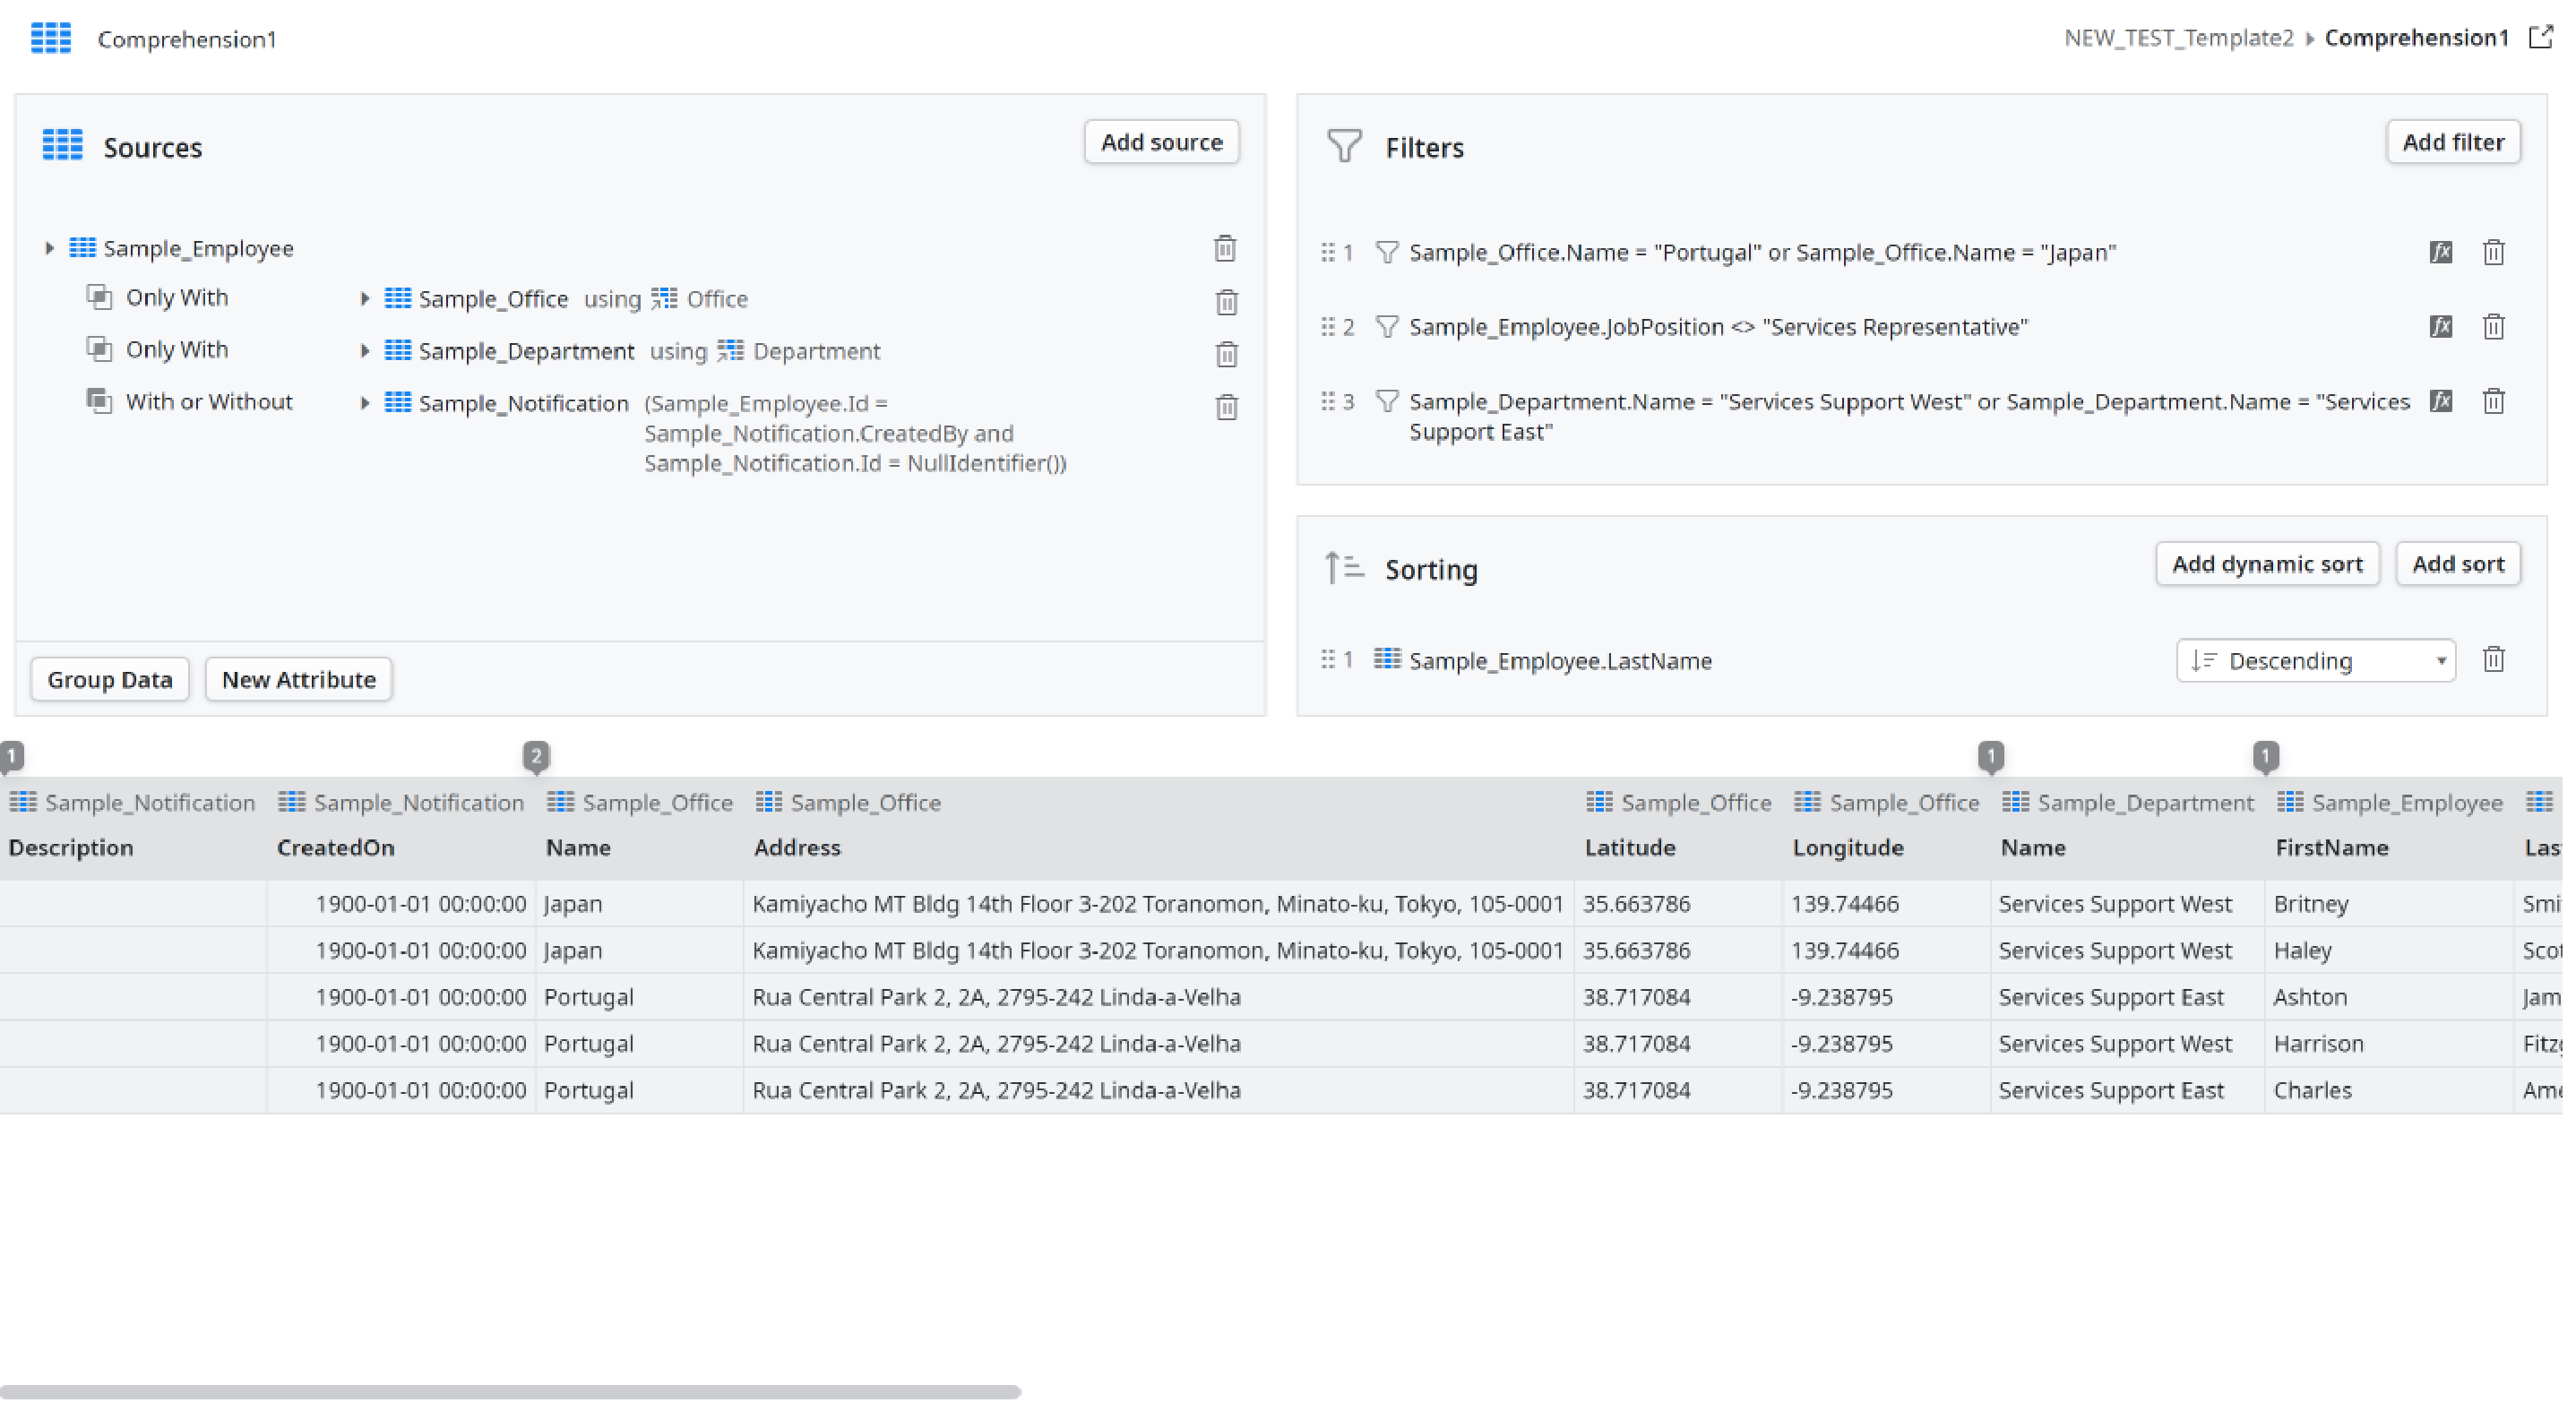
\includegraphics[height=3.0in]
  {final-c1}
	\caption{Example of a query that contains a join condition edited manually: The join condition between $"Sample\_Employee"$ and $"Sample\_Notification"$ was edited so this condition was not simplified as the other ones.}
	\label{fig:finalC1}
\end{figure}

%Modal

Finally on this point concerning the foreign keys of the joins, there was a problem in the existing interface which could lead users to make semantic errors while they are formulating queries that uses entities which could be joined using different foreign keys. As explained in \ref{subsec:paper_prototype_implementation}, the existing interface did not ask users which foreign key he wants to use. Consequently, the idea adopted in the paper prototype (Figure \ref{fig:paperFkSelect}), which had leveraged the results for the user testing in a positive way, continued to this phase, where a modal appears in cases where there are multiple foreign keys, asking user which attribute he would want to use to merge the entities, as demonstrated in Figure \ref{fig:foreignKeyModal}.

%Figure chave estrangeira modal

\begin{figure}[htbp]
	\centering
  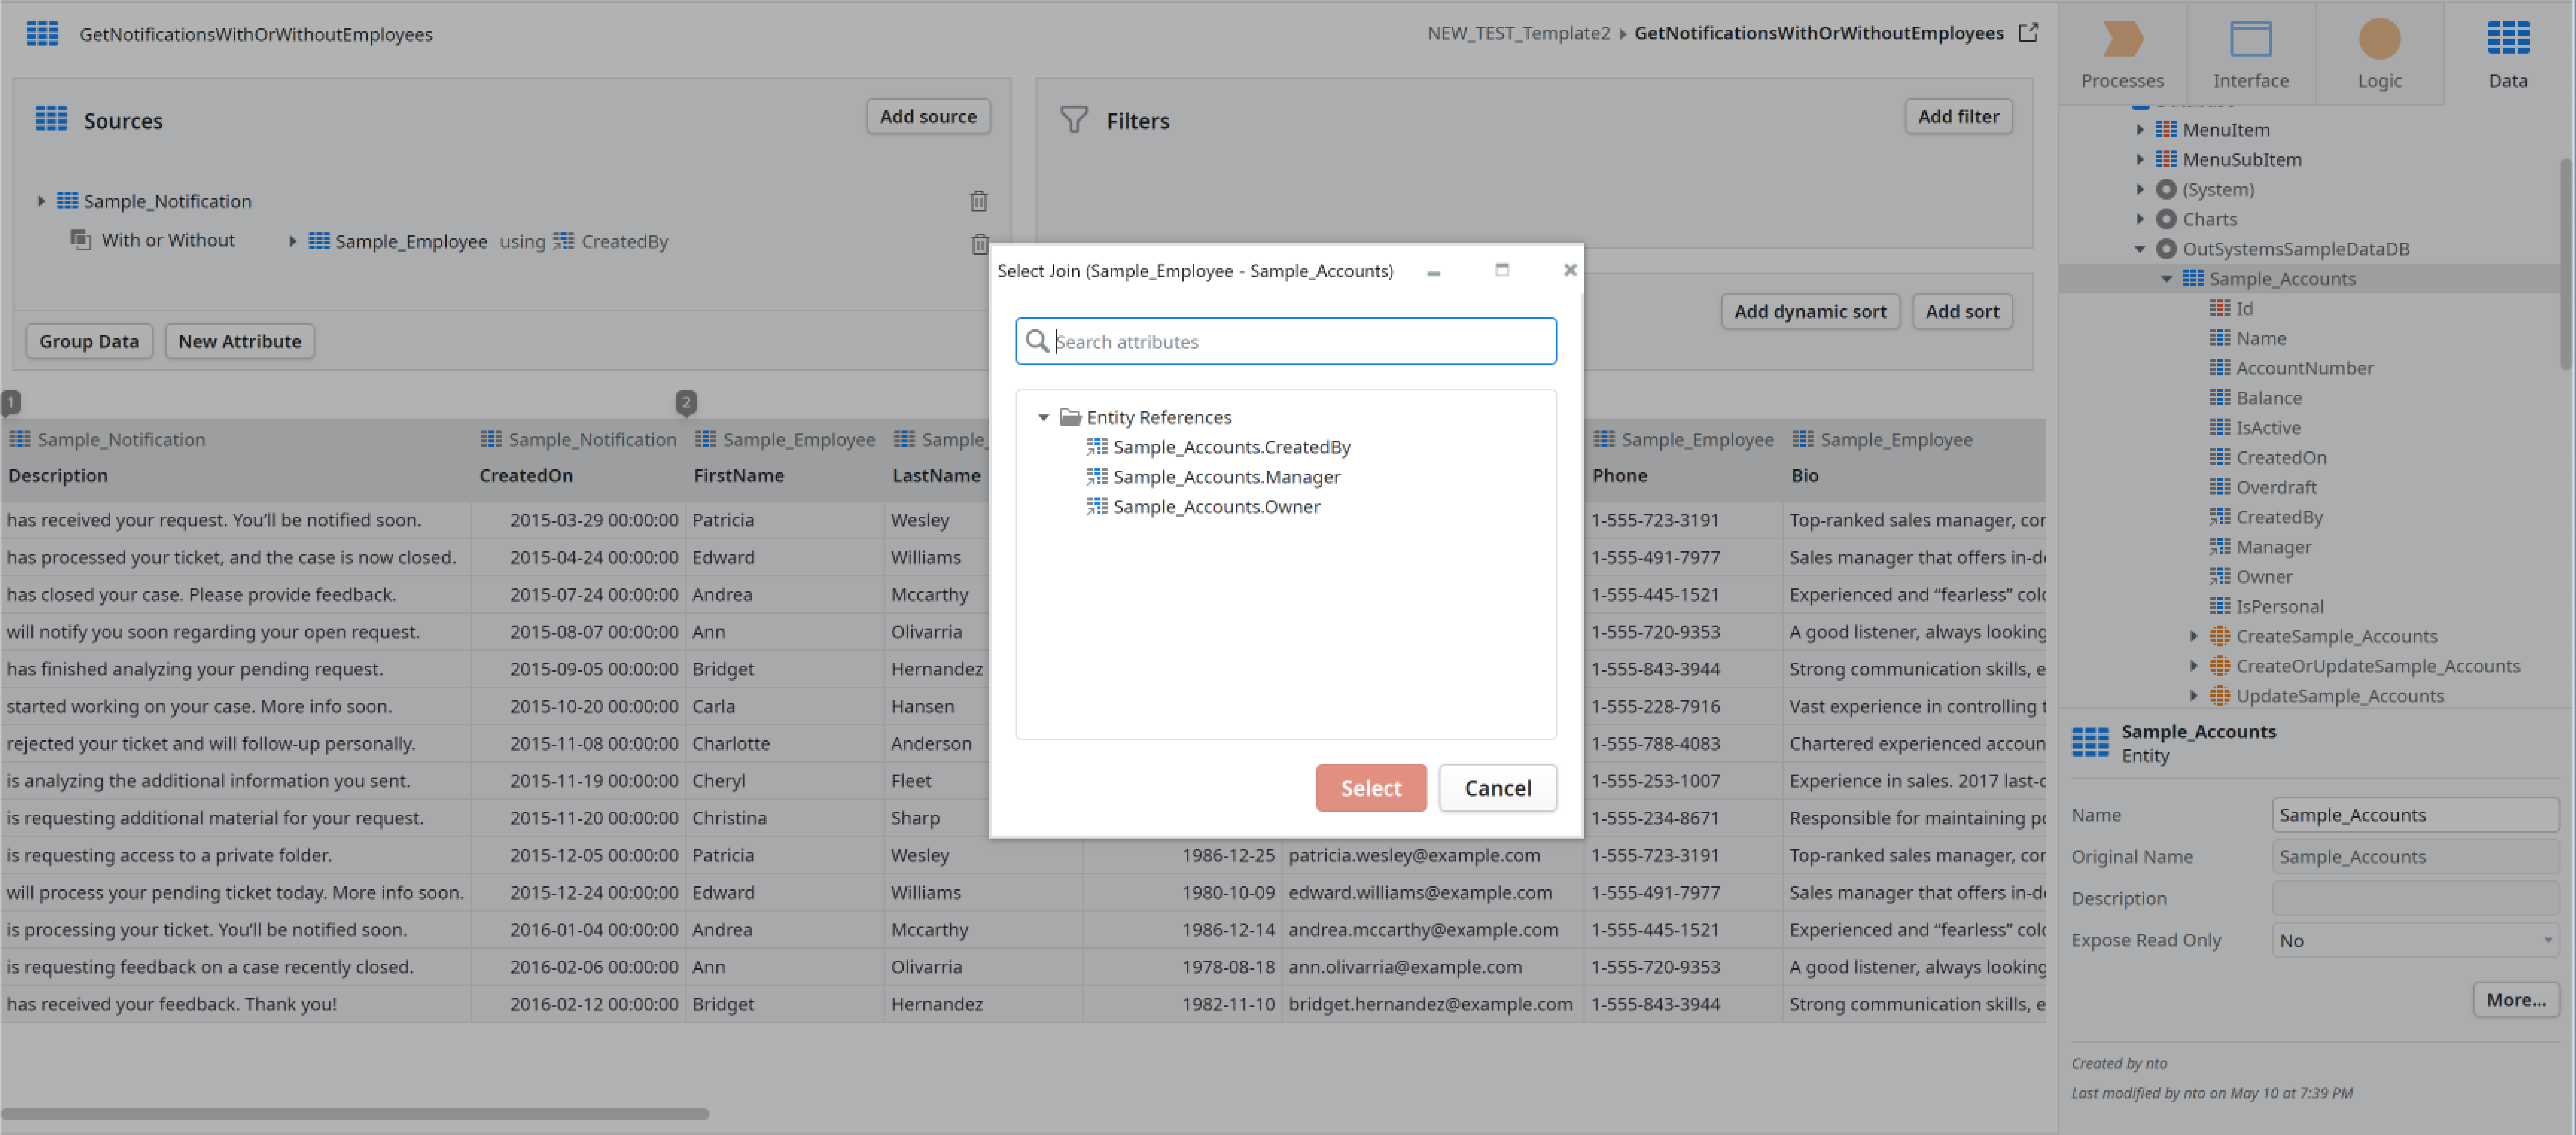
\includegraphics[height=2.5in]
  {foreign-key-modal}
	\caption{Modal that asks user which foreign key attribute he wants to use to merge the two entities. In the example illustrated, the user has already added $"Sample\_Notification"$ and $"Sample\_Employee"$, and when he added $"Sample_Account"$ the interface showed the modal presented since there are three references of employees on the account entity: $"CreatedBy"$, $"Manager"$, and $"Owner"$.}
	\label{fig:foreignKeyModal}
\end{figure}

Moreover, the $"Source"$ component was changed to present every entity as a tree node which contains the name and icon of each attribute as a child. Besides, not only a context menu, available when users right-click in each entity attribute, was added, as Figure \ref{fig:finalNewRightClick} exemplifies, but also an option to click on the attribute to highlight it on the query result preview. In that way, there is a possibility to find and add query options easier, since the table auto-direct the user to the intended attribute, promoting a more quick right-click on the attribute to apply aggregation functions, group bys, filters, sorting, or even to hide it.

\begin{figure}[htbp]
	\centering
  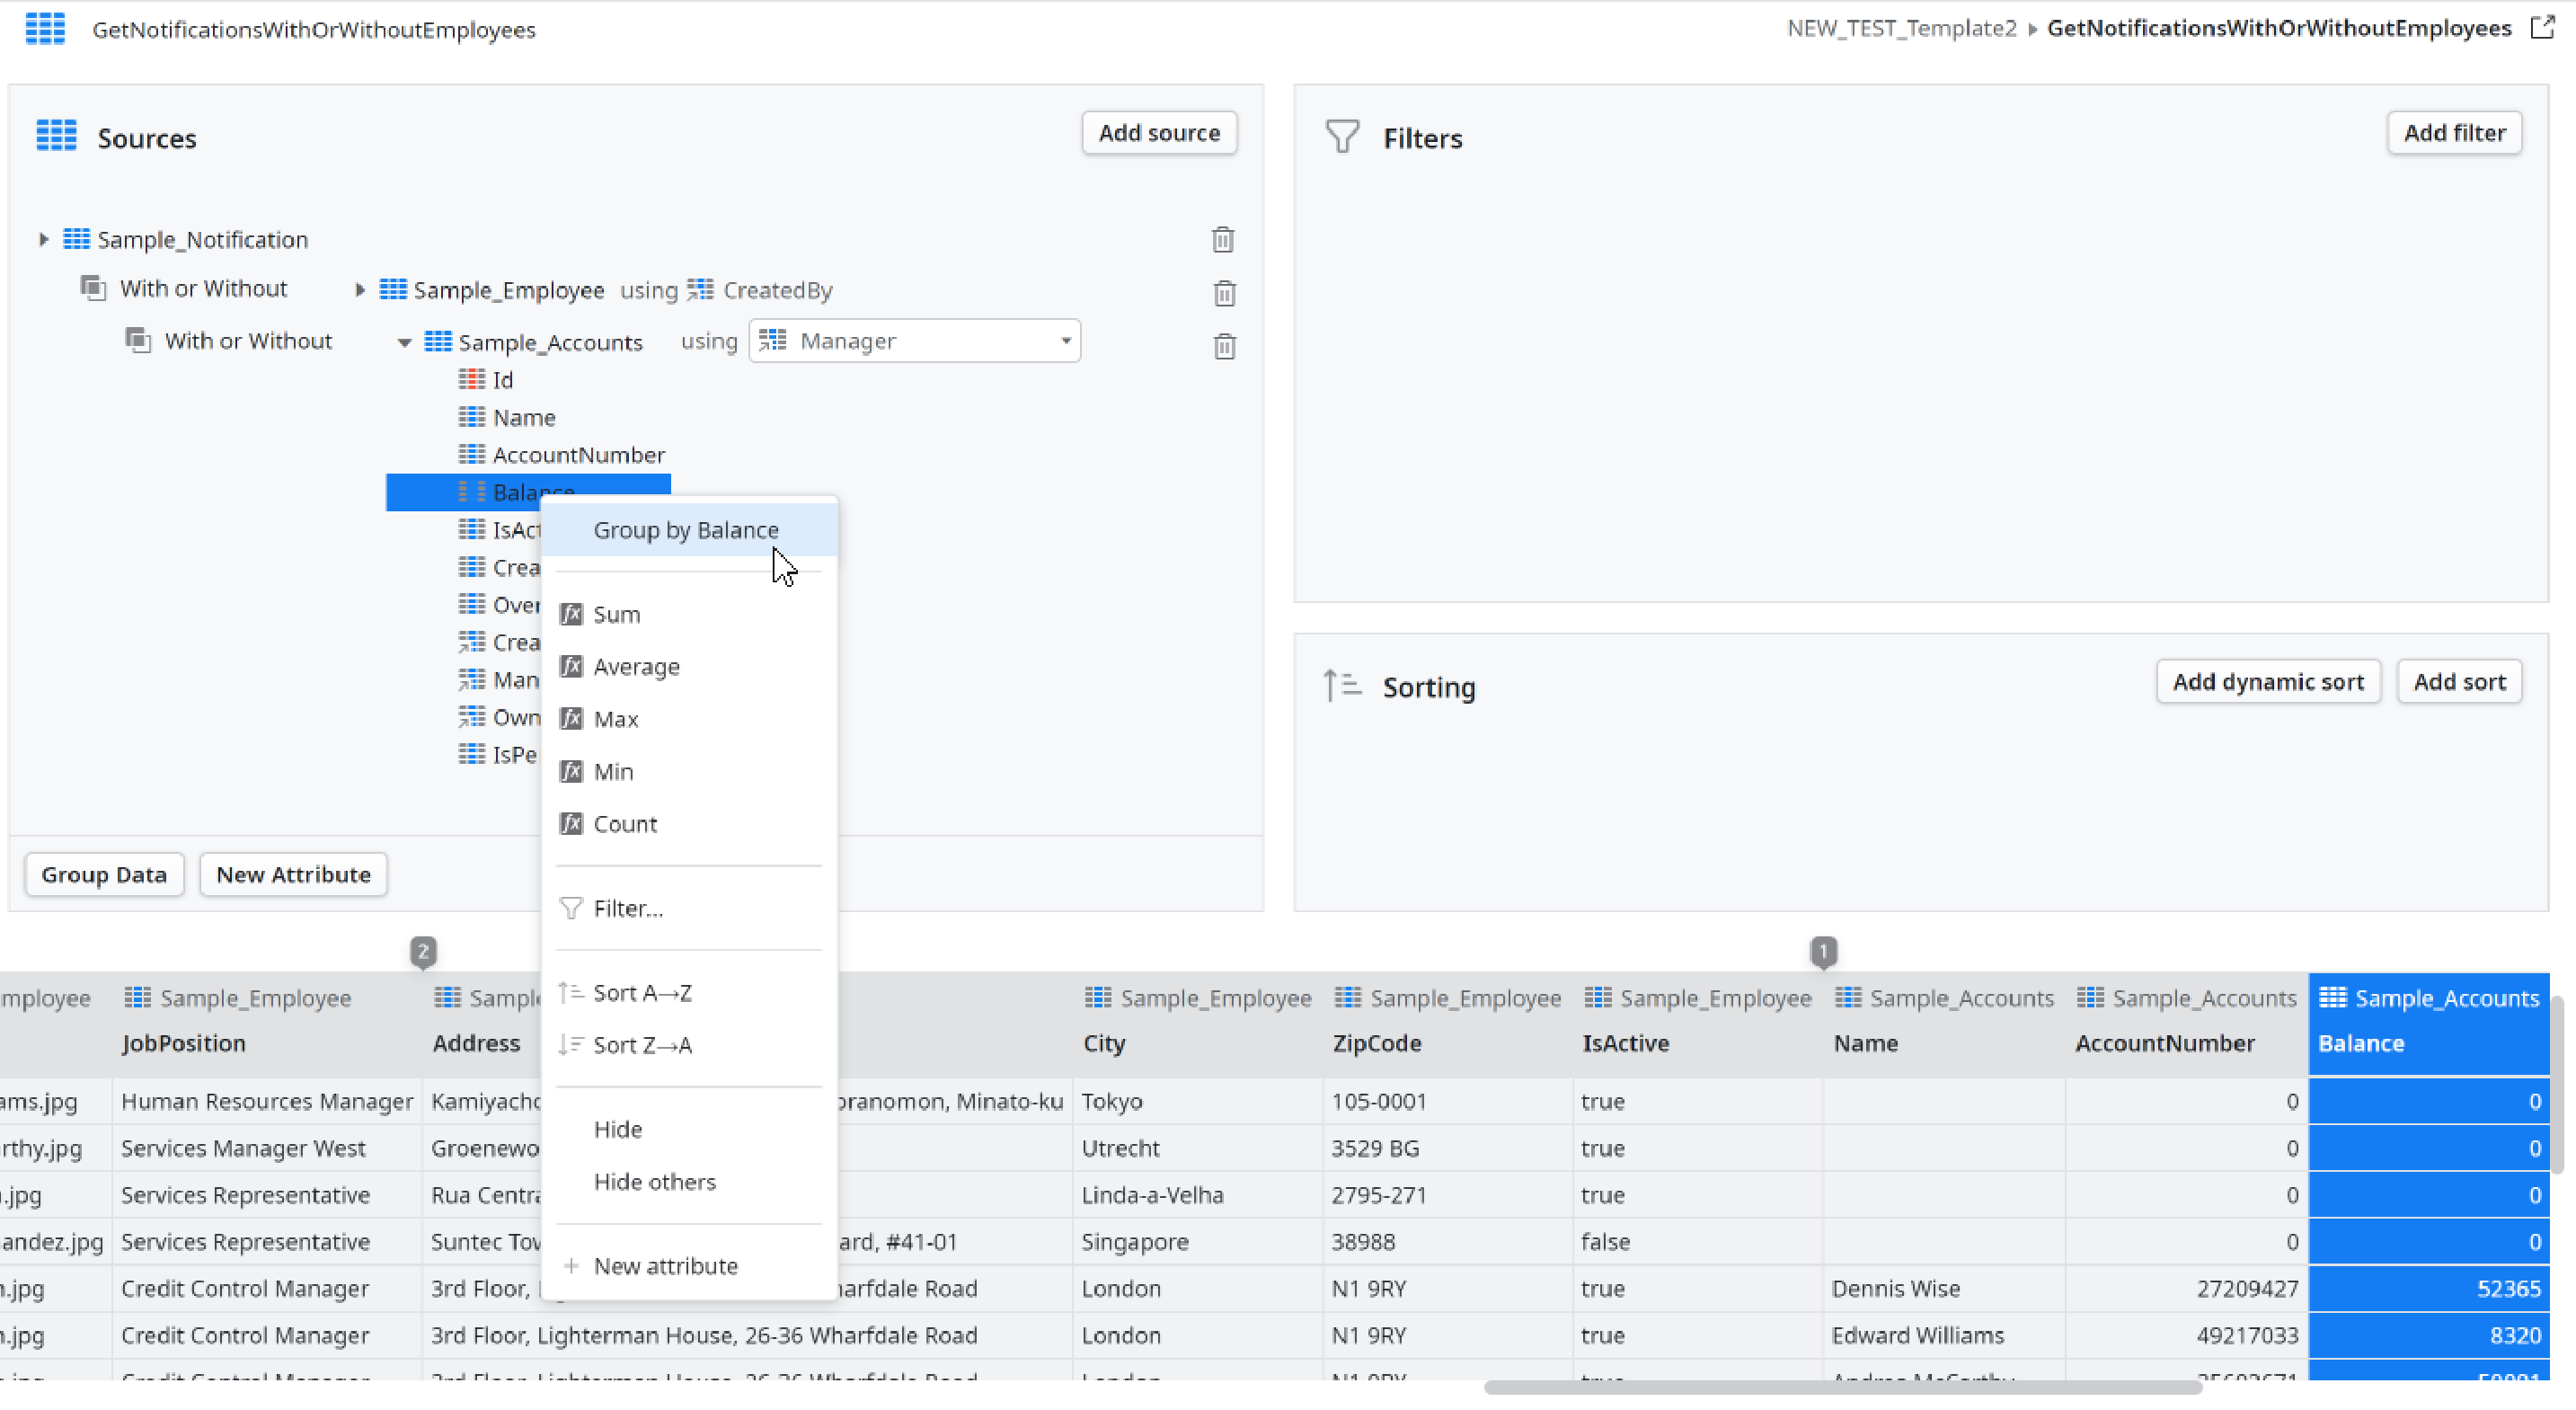
\includegraphics[height=3.0in]
  {final-new-right-click}
	\caption{Attributes of each entity and interactions accessible using the right click to trigger the context menu.}
	\label{fig:finalNewRightClick}
\end{figure}

\medskip

\textbf{New alternatives to add and search for attributes:}

\medskip

Nevertheless, these options not only are interesting alternatives to access these functionalities of the query builder, but also add a visible way to access these options, which will improve the adoption of new users when they try to use the system. As stated before, these options were added in the Paper Prototype, as illustrated in \ref{fig:paperAddAggregation} and \ref{fig:paperAddCalculatedAttribute}. However, as mentioned in \ref{subsec:paper_prototype_evaluation}, some users did not understand if they would need to add a calculated attribute or an aggregated attribute. Consequently, the button labels were changed to provide a more imperative and informative message related to the action accessible through each button. In that way, "Add Aggregation / Group By" was changed to "Group Data" and "Add Calculated Attribute" was changed to "New Attribute", to reinforce that using the "Group Data" button users can combine data of an attribute merging its rows, and in "New Attribute", they can add a new attribute calculated from the existing ones to the query result. Besides, tooltips were also added to each button in order to clarify the users who were confused about what function they intend. Figure \ref{fig:newButtonsTooltips} illustrates the two buttons and the respective tooltips added.

%Figure with two sub figures to show the tooltips of the two buttons (group data and new attribute).

\begin{figure}[tb]
  \centering
  \subcaptionbox{New Attribute\label{fig:groupDataTooltip}}%
    {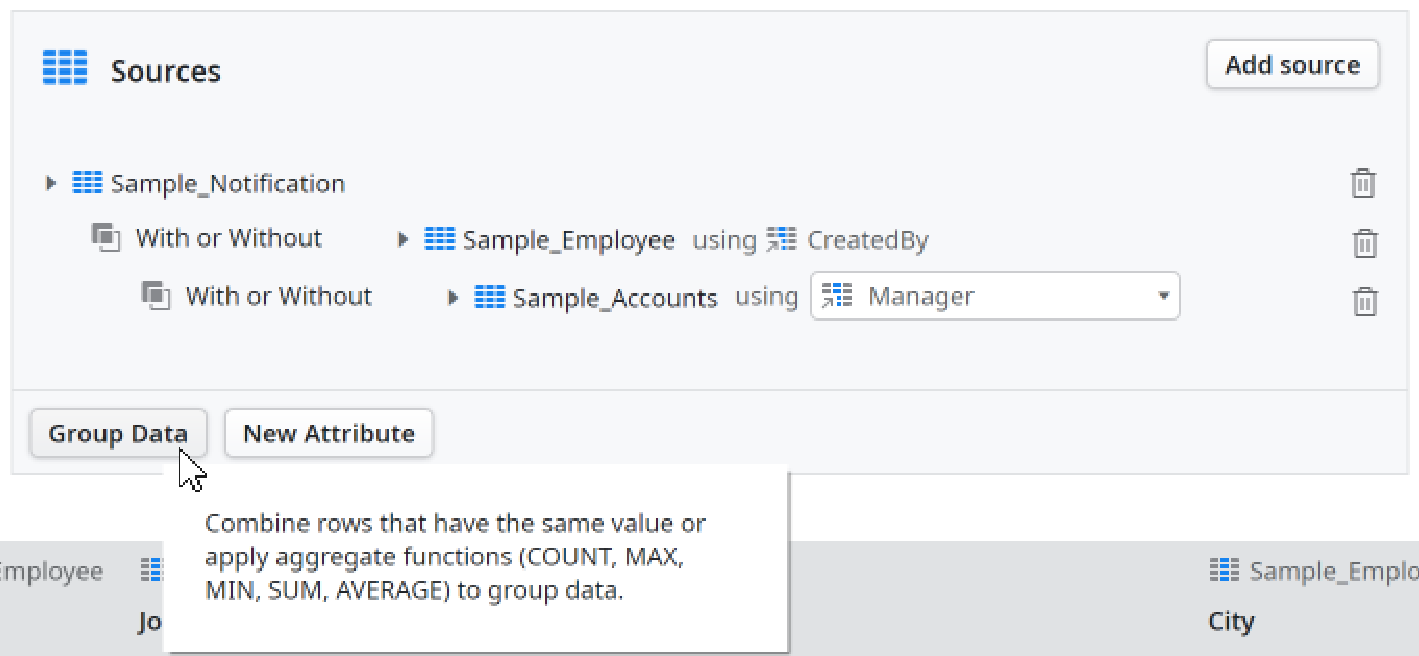
\includegraphics[height=1.3in]{group-data-tooltip}}%
  \subcaptionbox{Group Data\label{fig:newAttributeTooltip}}%
    {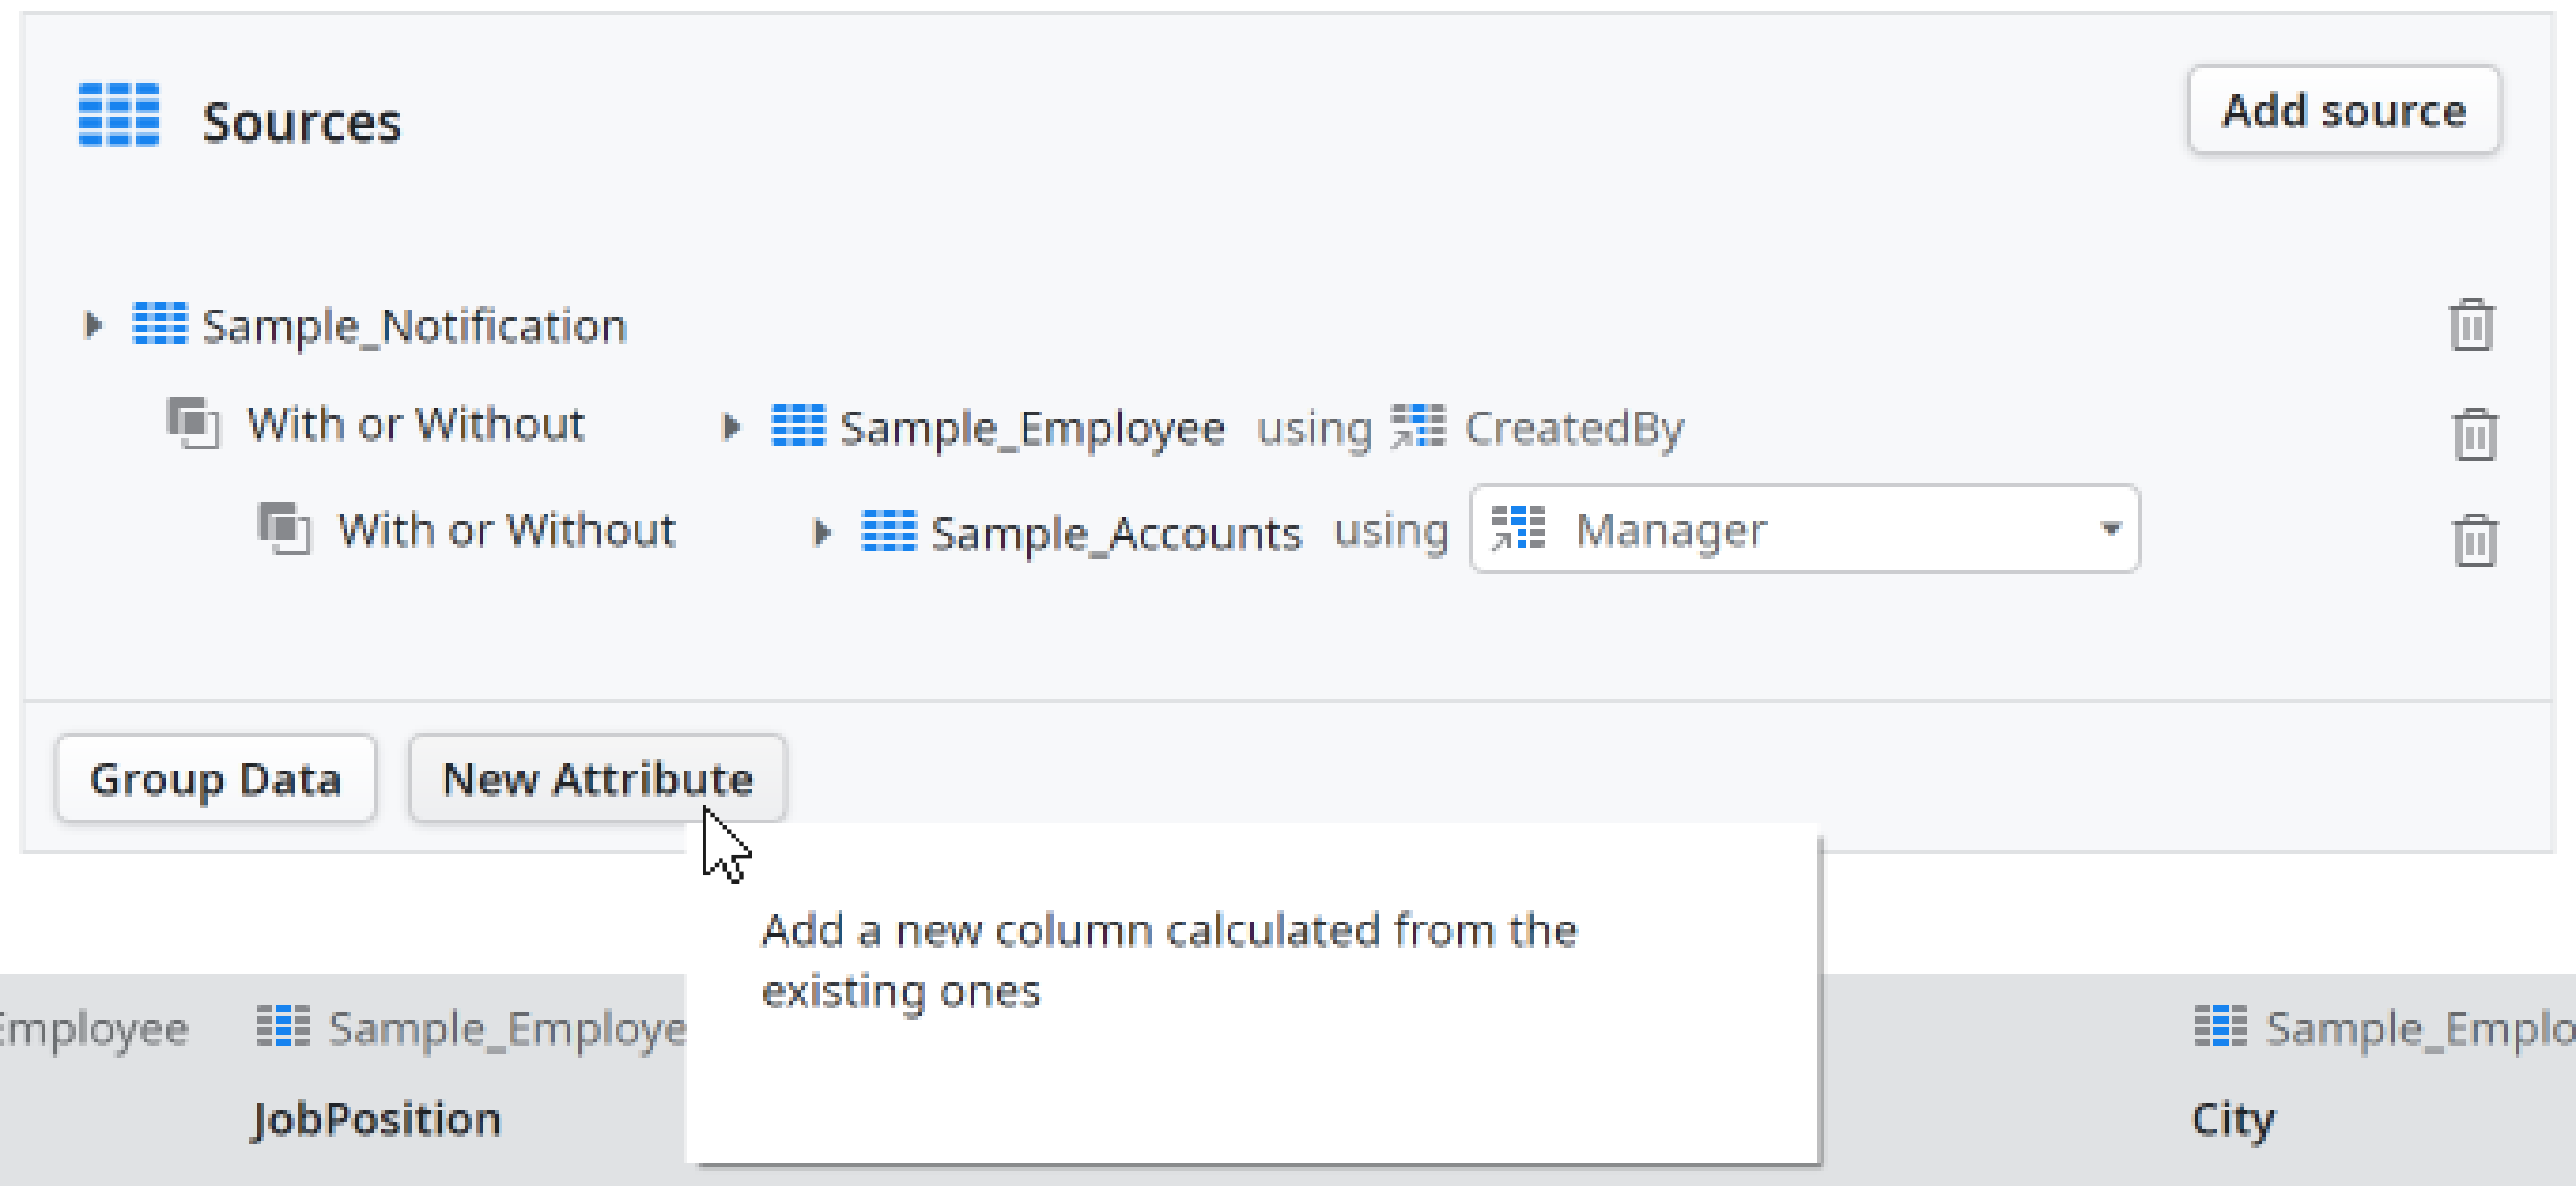
\includegraphics[height=1.3in]{new-attribute-tooltip}}%
\caption{Tooltips of the two new buttons added.}
  \label{fig:newButtonsTooltips}
\end{figure}

When a user click on the "Group Data" button the area, the interface shows a new area where the user can select the attribute and the functions he could apply to the attribute according to the attribute data type. Figure \ref{fig:groupDataEditor} demonstrates this new designed functionality of the system. This option is advantageous not only for users who are not familiarized with the system, who can see a visible option to group data, but also is it provides a faster way to add multiple group bys or aggregation functions since in a short area of the interface users can group data of several attributes without the need to search horizontally through the query result.

%Figure illustrating the group data area

\begin{figure}[htbp]
	\centering
  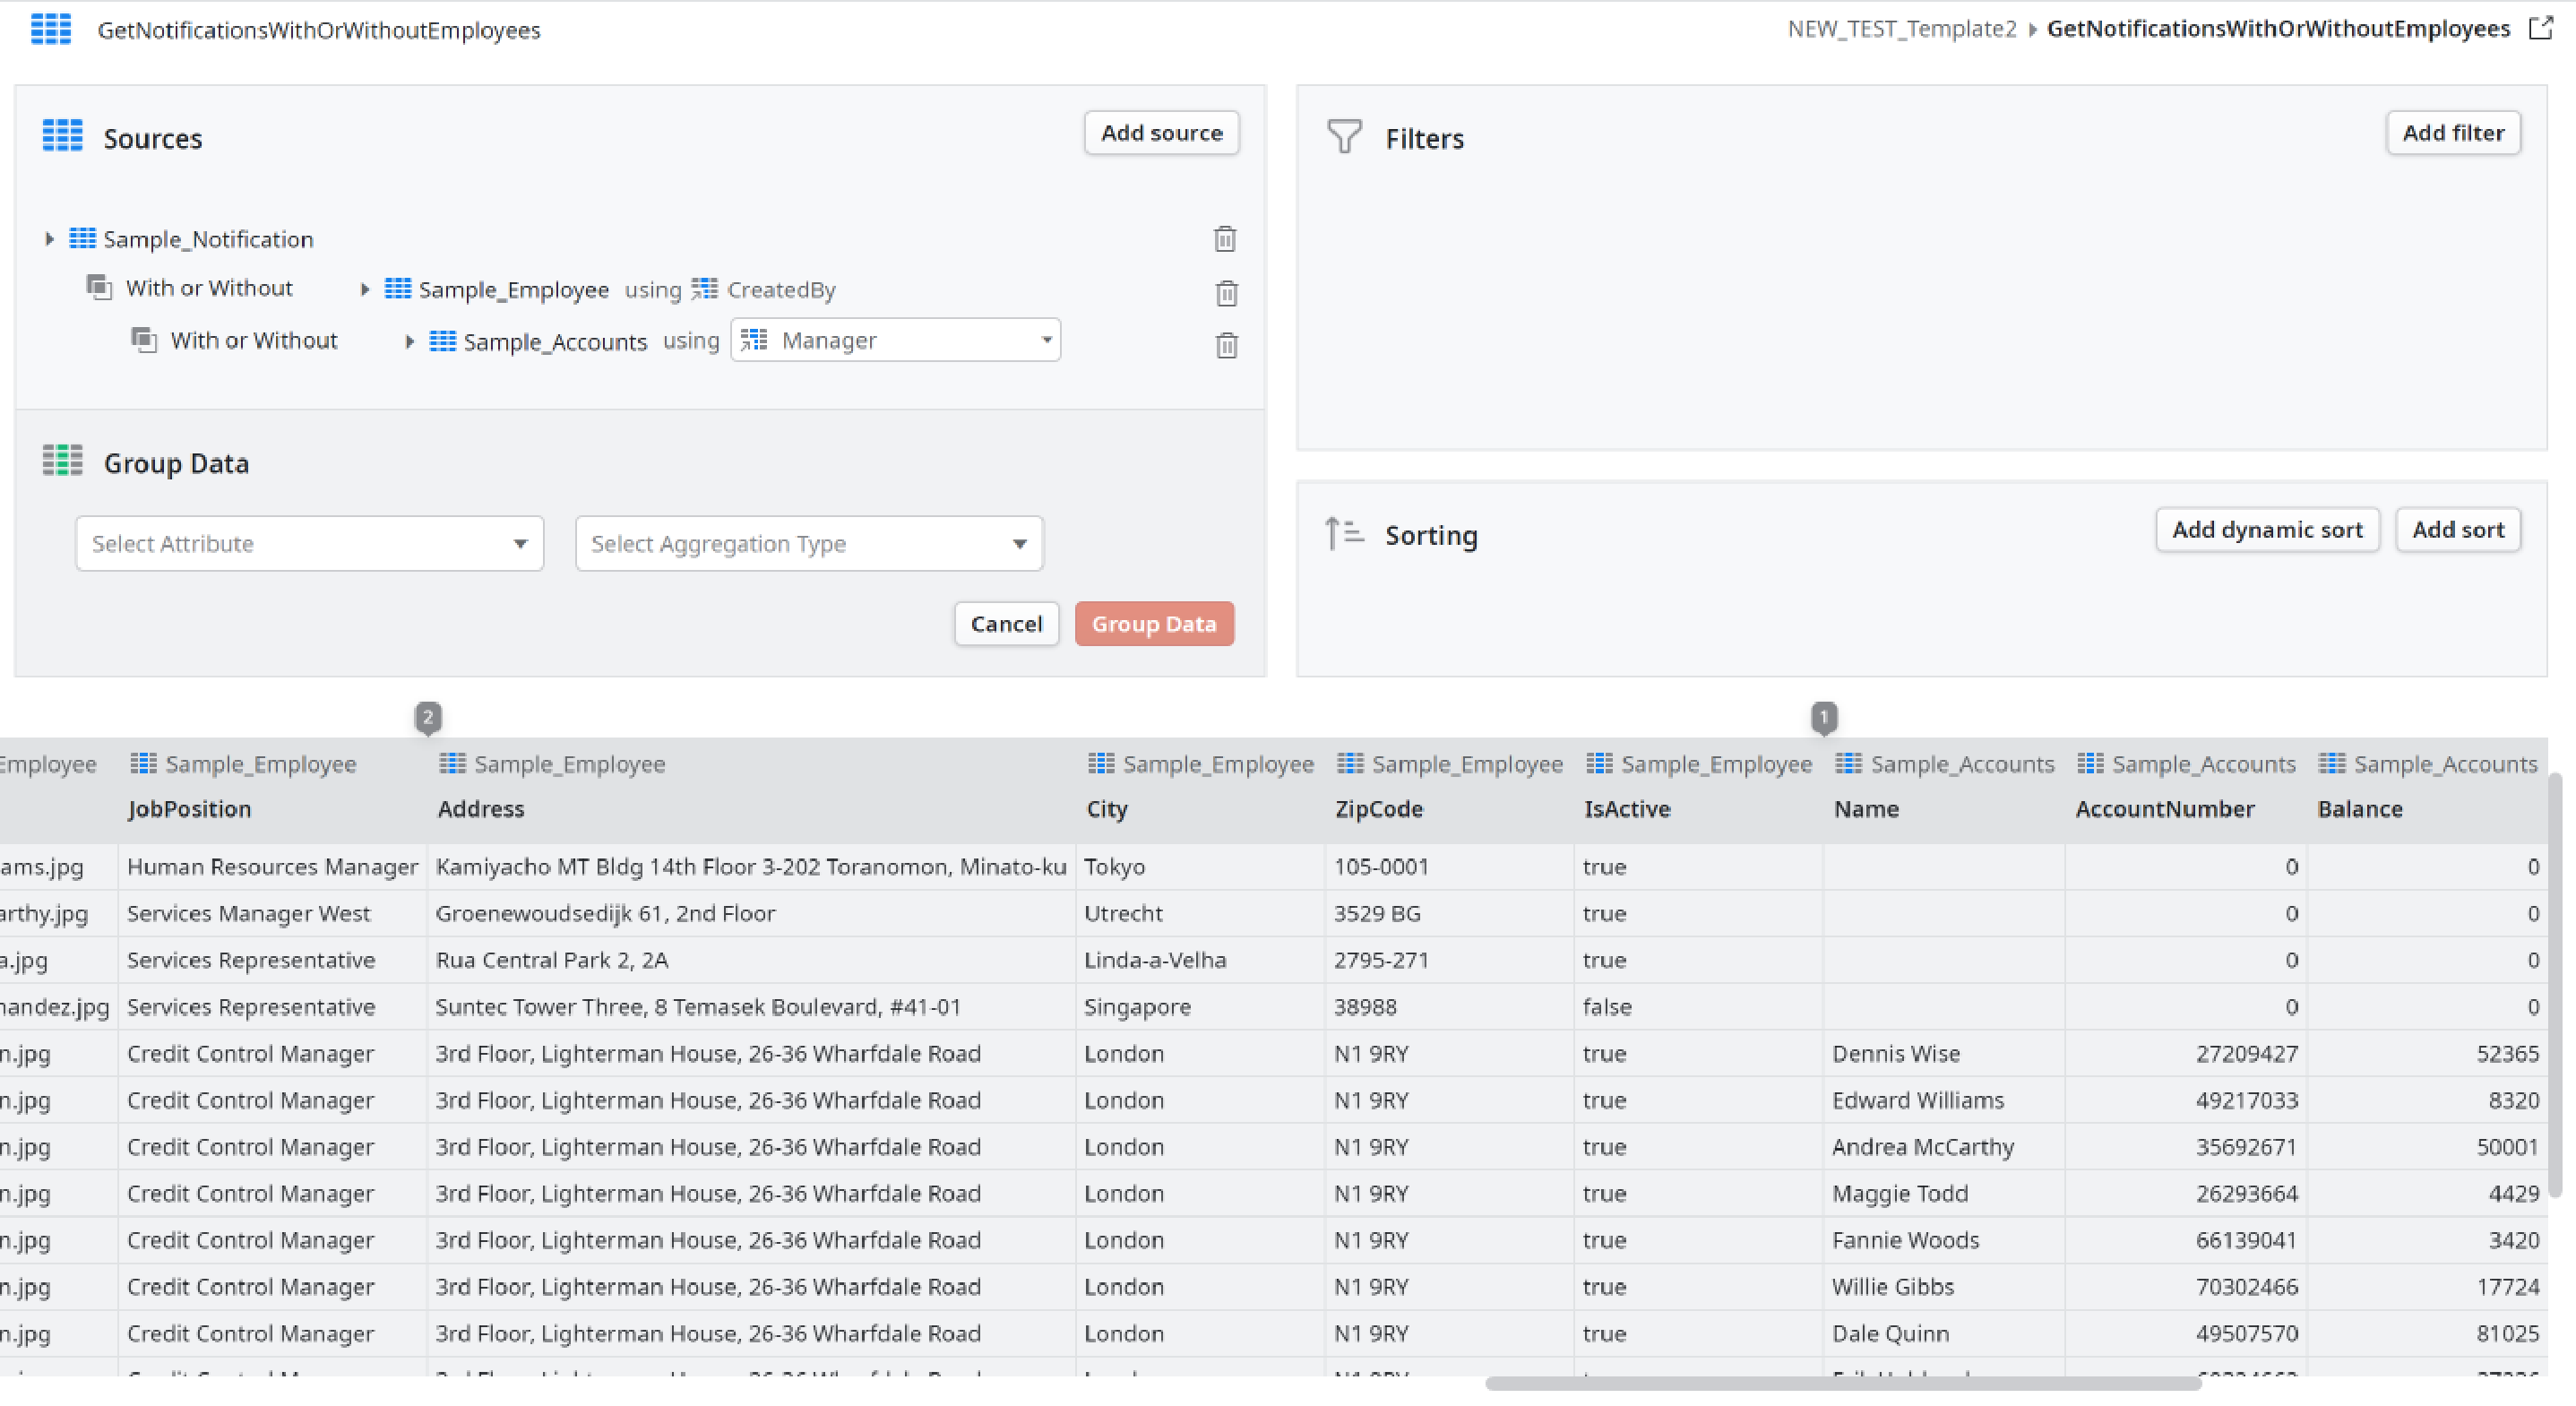
\includegraphics[height=3.0in]
  {group-data-editor}
	\caption{New alternative to group data.}
	\label{fig:groupDataEditor}
\end{figure}

The "New Attribute" button allows users to add calculated attributes in the same way they could add it before using the button available at the right side of all columns (in most times hidden due to the overflow). However, this button not only is more visible but also is more accessible.

The attributes added through these two buttons over the query formulation process are presented in the "Sources" tab, as illustrated in Figure \ref{fig:finalStructuredAttributes}. This representation is advantageous since users can read more information about how those attributes were added because there are visible information about the attributes and the formulas used to insert them.

%Figure illustrating how calculated attributes and aggregated attributes are represented in the interface. Put squares and identifications of the parts in FIGMA

\begin{figure}[htbp]
	\centering 
  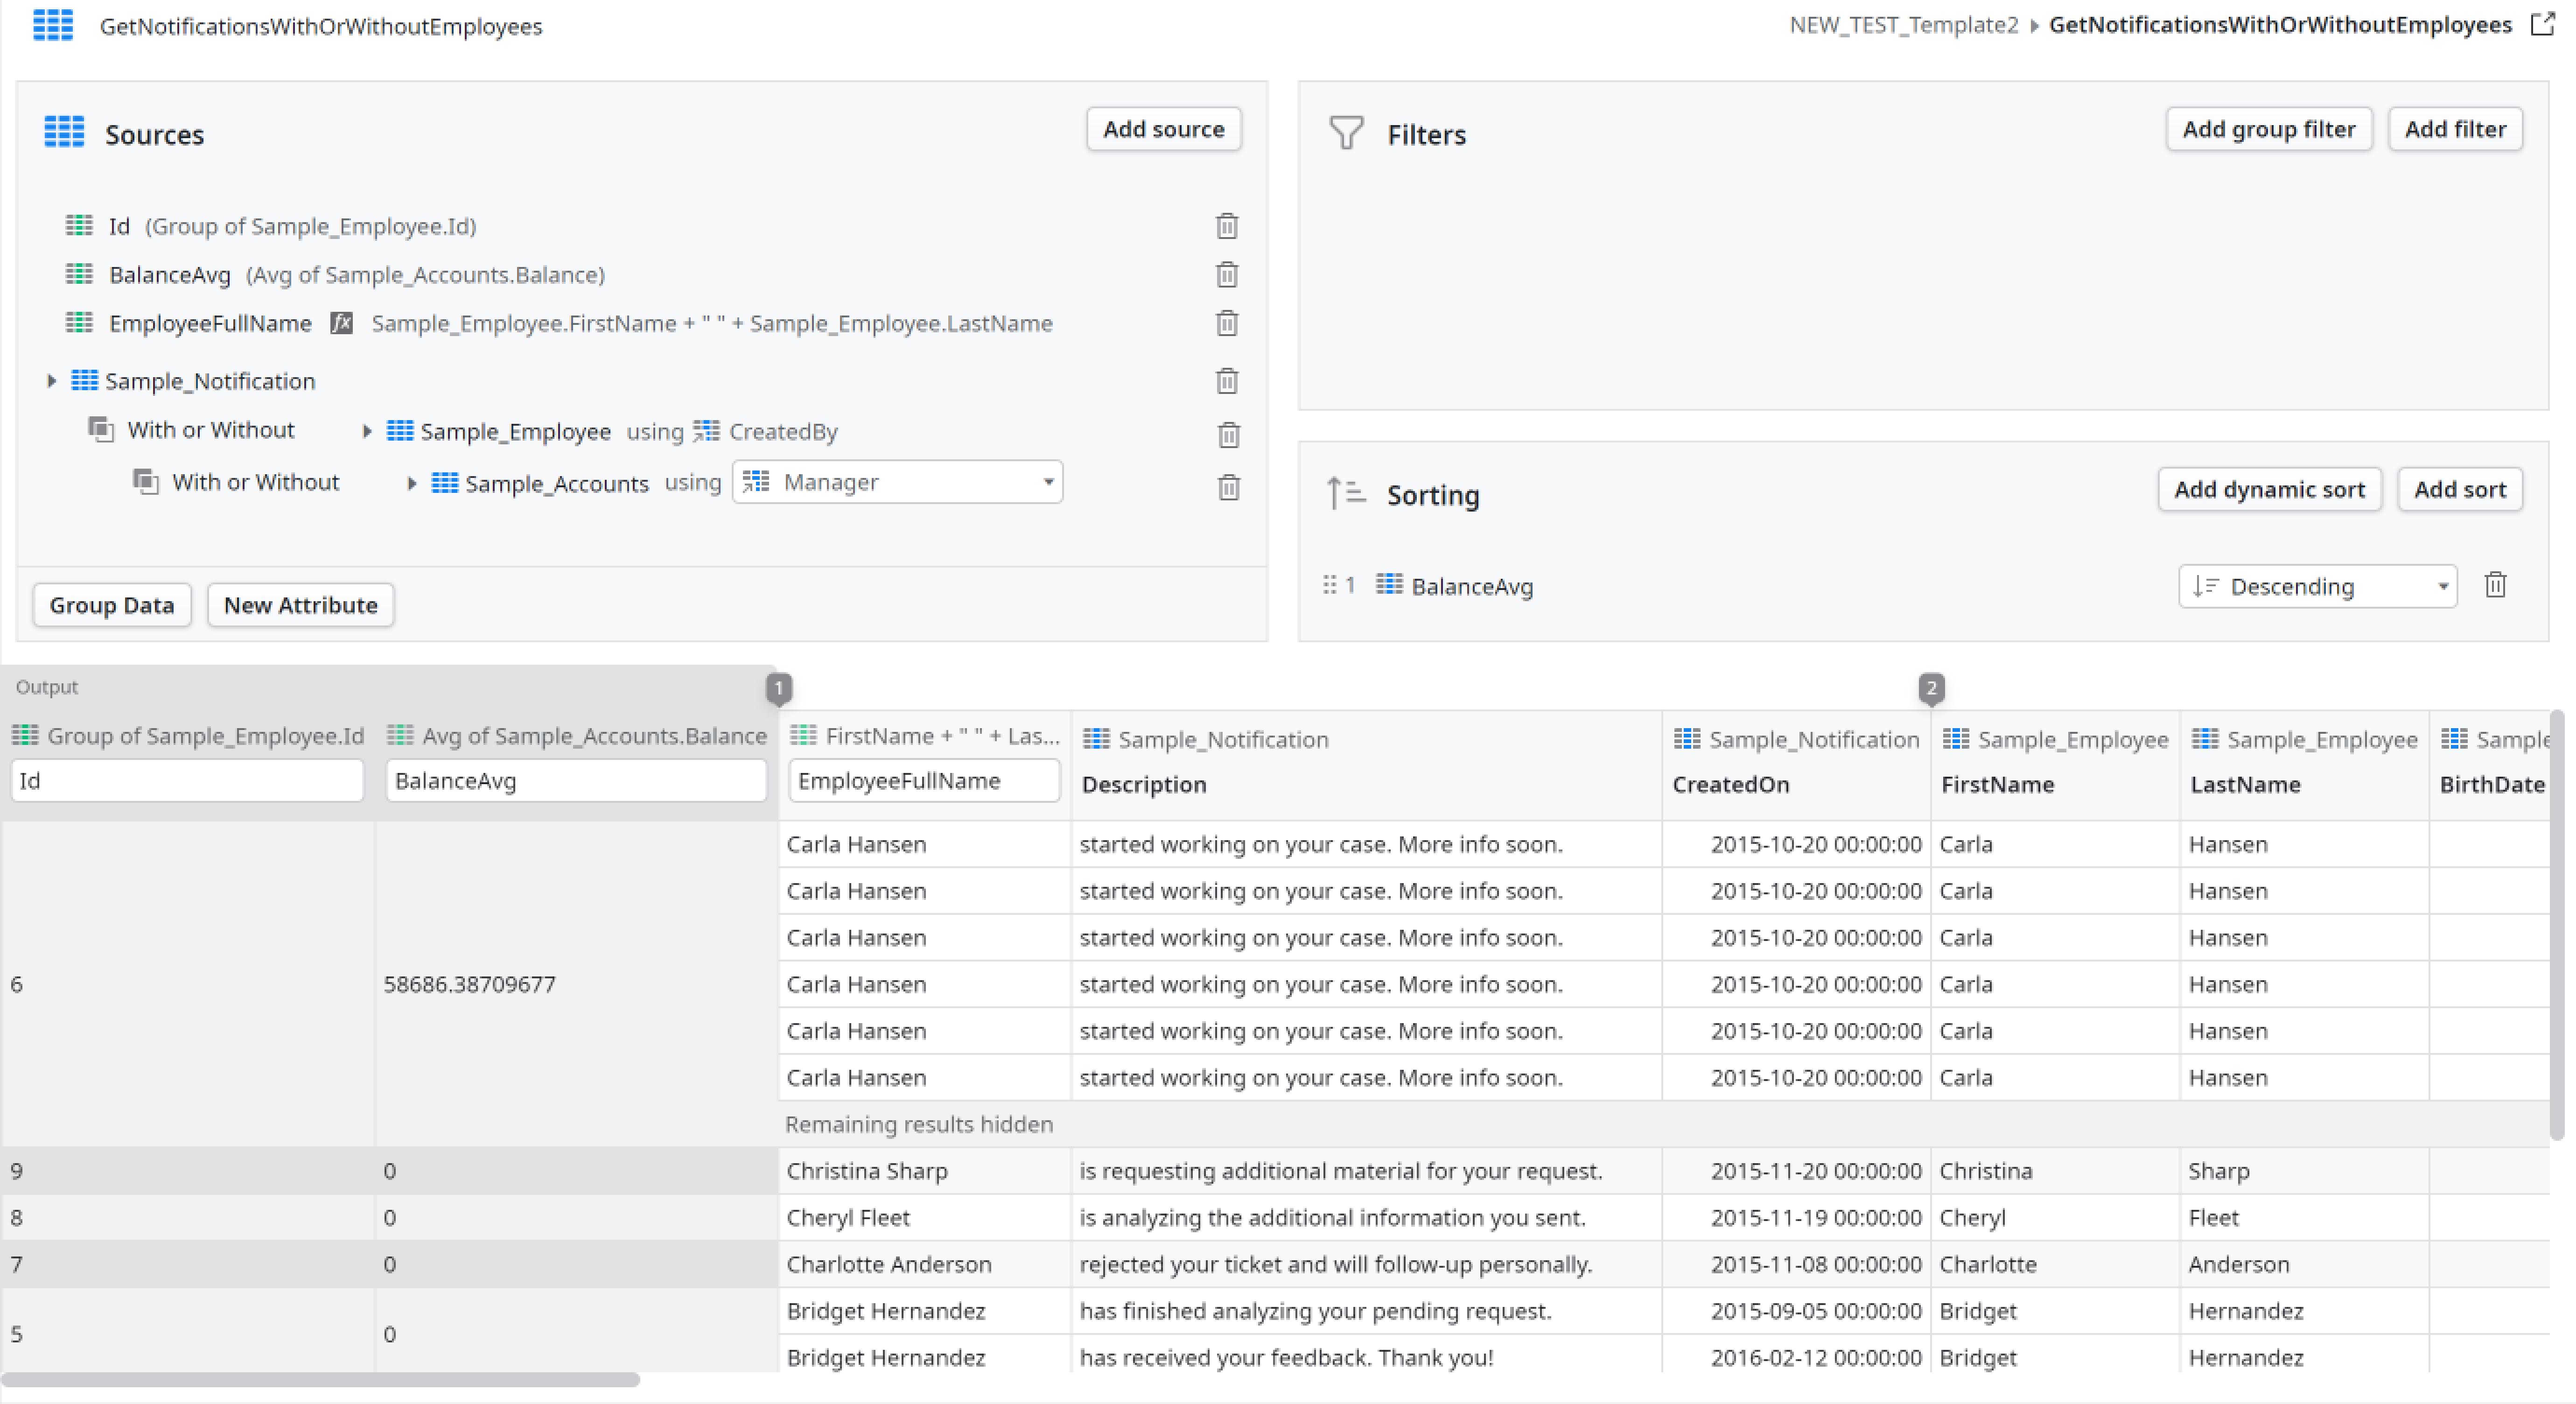
\includegraphics[height=3.0in]
  {final-structured-attributes}
	\caption{Example of a query that contains a group by ($"Id"$), an aggregation function ($"BalanceAvg"$) and a calculated attribute ($"EmployeeFullName"$).}
	\label{fig:finalStructuredAttributes}
\end{figure}

In the same way, the query result table headers of these attributes were changed not only to improve their readability but also to maintain the consistency with the new area visible in sources. Figure \ref{fig:groupHeadersComparison} compares the header representation of an aggregated attribute, a group by, and a calculated attribute in the existing interface to the new one. As can be observed, the reference of the source attribute used to group data was added to the group bys and aggregation function, since before it was difficult to perceive which attributes were grouped in the query. Moreover, the function symbol of aggregation functions was removed since no formula is inserted in these attributes and several users tried to click on the function symbol to open some formula.

\begin{figure}[tb]
  \centering
  \subcaptionbox{Existing Interface\label{fig:existingGroupHeaders}}%
    {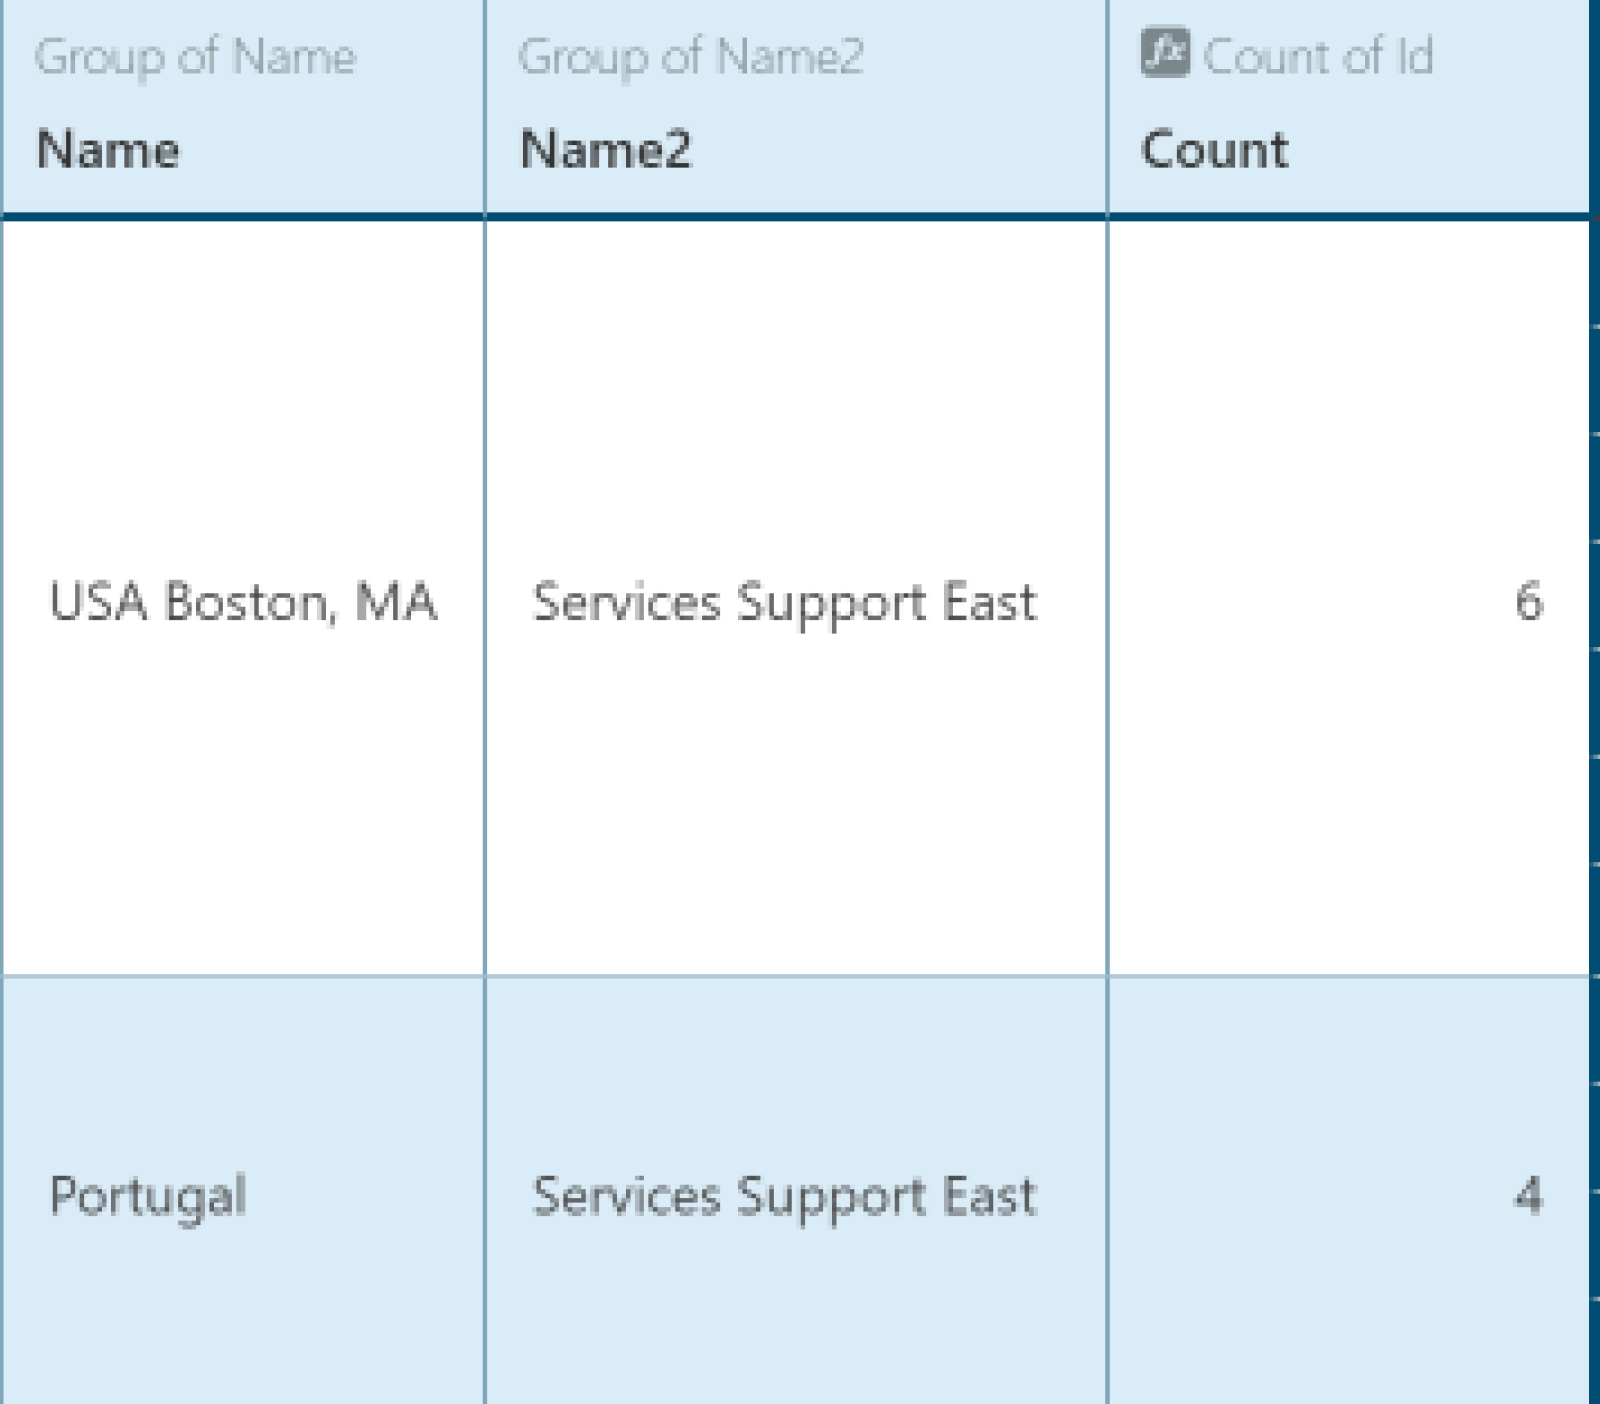
\includegraphics[height=1.5in]{existing-group-headers}}%
  \subcaptionbox{Service Studio Prototype\label{fig:finalGroupHeaders}}%
    {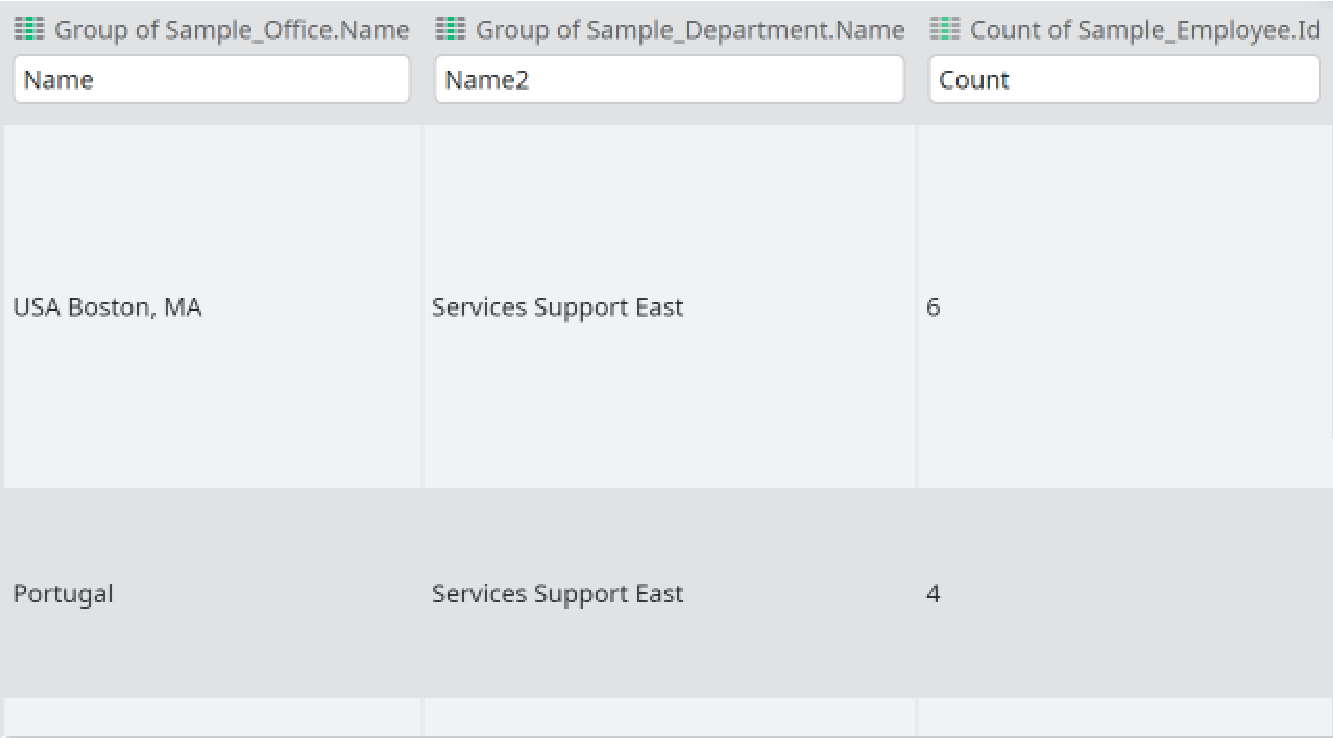
\includegraphics[height=1.5in]{final-group-headers}}%
\caption{Comparison between the table headers of the existing interface and the new ones (two group bys and one aggregated attribute, from the left to the right).}
  \label{fig:groupHeadersComparison}
\end{figure}


\subsection{Evaluation}
\label{subsec:service_studio_evaluation}

The final evaluation phase elaborated in the context of this dissertation was the usability tests of the final prototype, using the same methodology and testing scenarios used to test the existing interface and the paper prototype. Accordingly, the Final Prototype was tested with 30 users (10 users of each user group) under a remote environment supported by the Zoom \cite{zoom} meeting solution and its feature of sharing and recording the presenter's screen.

In that way, the users tried to accomplish the tasks integrated in the testing scenarios (detailed in Appendix \ref{app:user_testing_scenarios}) and all this interaction process was analyzed in order to perceive the difficulties they had as well as to register usability metrics that could allow to characterize the success of the prototype built and compare it with the previous visual querying solution.

%General overview

The users who use to the previous interface, have reacted positively to the new interface layout without tabs and the three areas always visible. They reinforced that in the previous interface it was very cumbersome to interpreter or formulate query using the tabs since they did not have a query overview anytime.

%Leitura sources view

In general, users who have some relational database foundations managed to comprehend effortlessly the new sources view, which presents all entities in a tree and promotes a more simple and compact view of the entities and joins included in the query, and pointed out that the arrangement used allow to perceive faster the query purpose since it is possible to visualize which entities are related with each other.

The changes applied to the foreign key used in the joins generated automatically have impacted positively the users' success rate performing scenarios that contain these cases. For example, as Table \ref{tab:finalPrototypeForeignKeyIdentification} details, the 58.89\% of users have identified the foreign keys used to merge tables that could be linked using different attributes. On the other hand, the modal added to ask user which foreign key he intend to use when there are multiple available options to create the automatic join, have improved the effectiveness of the join insertion for these cases. For instance, Table \ref{tab:finalPrototypeForeignKeySelection} demonstrates the effectiveness of the join specification of the F1 scenario where is necessary to join two entities using a specific foreign key and these two entities have three relationships linking each other. As it can be observed, the results are very positive since 96.67\% of users have joined the two entities used the required foreign key. In that way, this change of the interface have leveraged the guidance that the interface could give to users reaching their goals, mainly in these cases where a distraction could lead to query the wrong data, turning the interface less error-prone.

Nevertheless, the approach used to distinguish the joins generated automatically to the ones that were edited manually and have a more complex condition have not relevead positive results. As Table \ref{tab:finalPrototypeLeftJoinNull} presents, in the use case used to present a join edited manually, only 16.67\% of users have successfully interpreter the join purpose.


%Relational database knowledge / Success 

Regarding the operations which were identified as difficult to find by users who have never used the query builder neither visualize any tutorial video concerning it (add group by, aggregation function or calculated attributes), the majority of users managed to find intuitively the options to access this functions in the scenarios they needed it.

As presented in table \ref{tab:finalPrototypeCalculatedAttribute}, 83.33\% of users added calculated attributes when necessary without difficulties and no user did not manage to add it. At the same way, users have less dificulties to apply aggregation functions and group bys, since the two buttons were visible in the interface and they found them easily. In that way, the main cause for users did not manage to group data was the lack of relational database knowledge.

%TODO Probably, chart of relational database knowledge and F1 success

The new functionality added that allow users to search for a specific attribute and apply operations using the attributes tree was not found intuitively. Several users thought that the "triangle" buttons to expand the attributes of an entity were to add information regarding the join of the entity and the nested one.

However, after ending the test, this functionality was demonstrated to the users and they revealed that is very useful although they did not discover the feature by themselves. In that way, it is necessary to add some introduction to indicate that this functionality is available or study other representations that could be more intuitive for users.

In conclusion, Table \ref{tab:effectiveness_final_prototype} and Figure \ref{fig:effectivenessFinalPrototypeUserGroup} summarize the average of the success of each user group in each scenario as well as the total average. OutSystems Developers achieved 81.43\% of the scenarios, Software Developers 68.57\%, and Citizen Developers 50\%. Considering all user groups, 66.67\% of the scenarios were completely achieved and 7.90\% have not completely achieved due to the lack of some peculiarities. The success was classified according to the Table \ref{tab:effectiveness_states} already presented and the description of user testing scenarios and user groups which are detailed in Appendix \ref{app:user_testing_scenarios} and in section \ref{sec:target_users} respectively.


% Please add the following required packages to your document preamble:
% \usepackage{booktabs}
\begin{table}[tb]
  \caption{Success rate of users when they needed to add a calculated attribute. (Final Prototype usability tests - 30 users)}
    \label{tab:finalPrototypeCalculatedAttribute}
  \begin{tabular}{@{}lrrr@{}}
  \toprule
  \textbf{Insert Calculated Attribute} & \multicolumn{1}{l}{Added Successfully} & \multicolumn{1}{l}{Difficulty to Add} & \multicolumn{1}{l}{Could not Add} \\ \midrule
  OutSystems Developer                 & 100.00\%                               & 0.00\%                                & 0.00\%                            \\
  Software Developer                   & 70.00\%                                & 30.00\%                               & 0.00\%                            \\
  Citizen Developer                    & 80.00\%                                & 20.00\%                               & 0.00\%                            \\
  Total                                & 83.33\%                                & 16.67\%                               & 0.00\%                            \\ \bottomrule
  \end{tabular}
  \end{table}





% Please add the following required packages to your document preamble:
% \usepackage{booktabs}
\begin{table}[tb]
  \caption{Readability of the foreign keys used to join entities that could be joined using different attributes. (Final Prototype usability tests - 30 users)}
    \label{tab:finalPrototypeForeignKeyIdentification}
  \begin{tabular}{@{}lrrr@{}}
  \toprule
  \textbf{Foreign Key Identification} & \multicolumn{1}{l}{Identified} & \multicolumn{1}{l}{Did not Identify} & \multicolumn{1}{l}{Did not See the Join} \\ \midrule
  OutSystems Developer                & 86.67\%                        & 13.33\%                              & 0.00\%                                   \\
  Software Developer                  & 50.00\%                        & 50.00\%                              & 0.00\%                                   \\
  Citizen Developer                   & 40.00\%                        & 40.00\%                              & 20.00\%                                  \\
  Total                               & 58.89\%                        & 34.44\%                              & 6.67\%                                   \\ \bottomrule
  \end{tabular}
  \end{table}

% Please add the following required packages to your document preamble:
% \usepackage{booktabs}
\begin{table}[tb]
  \caption{Selection of the foreign key, in the formulation scenario, used to join entities that could be joined using different attributes. (Final Prototype usability tests - 30 users)}
    \label{tab:finalPrototypeForeignKeySelection}
  \begin{tabular}{@{}lrrr@{}}
  \toprule
  \textbf{Foreign Key Selection} & \multicolumn{1}{l}{Selected} & \multicolumn{1}{l}{Did not Select} & \multicolumn{1}{l}{Did not Add the Join} \\ \midrule
  OutSystems Developer           & 90.00\%                      & 0.00\%                             & 10.00\%                                  \\
  Software Developer             & 100.00\%                     & 0.00\%                             & 0.00\%                                   \\
  Citizen Developer              & 100.00\%                     & 0.00\%                             & 0.00\%                                   \\
  Total                          & 96.67\%                      & 0.00\%                             & 3.33\%                                   \\ \bottomrule
  \end{tabular}
  \end{table}

% Please add the following required packages to your document preamble:
% \usepackage{booktabs}
\begin{table}[tb]
  \caption{Readability rate of the join which represents the case where two entities were merged using a left join and the conditions specified the that the primary key of the right enitity must be null. (Final Prototype usability tests - 30 users)}
    \label{tab:finalPrototypeLeftJoinNull}
  \begin{tabular}{@{}m{5.4cm}rrr@{}}
  \toprule
  \textbf{Left Join with Null Identifier Comprehension} & \multicolumn{1}{l}{Identified} & \multicolumn{1}{l}{Did not Identiy} & \multicolumn{1}{l}{Did not seen the Join} \\ \midrule
  OutSystems Developer                                  & 30.00\%                        & 70.00\%                                & 0.00\%                                    \\
  Software Developer                                    & 20.00\%                        & 70.00\%                                & 10.00\%                                   \\
  Citizen Developer                                     & 0.00\%                         & 90.00\%                                & 10.00\%                                   \\
  Total                                                 & 16.67\%                        & 76.67\%                                & 6.67\%                                    \\ \bottomrule
  \end{tabular}
  \end{table}


\begin{figure}[htbp]
	\centering
	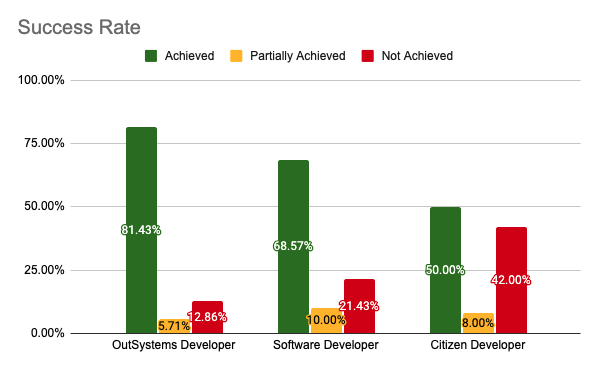
\includegraphics[height=2.8in]{effectiveness-final-prototype-user-group}
	\caption{Average of the success rate of all scenarios by each user group (Final Prototype usability tests - 30 users).}
	\label{fig:effectivenessFinalPrototypeUserGroup}
\end{figure}



\section{Results Analysis}
\label{sec:results_analysis}

The results obtained in usability tests of the existing interface, presented in \ref{sec:existing_interface_evaluation}, were compared against the results extracted from usability tests of the final prototype, presented in \ref{subsec:service_studio_evaluation}. The test environment was the same for both tests where 30 users (10 of each user group) tested the existing interface and different 30 users (also 10 of each user group) tested the final prototype. Accordingly, this section will present a comparison of the gathered metrics in the evluation of the two interfaces.

\subsection{Effectiveness}
\label{subsec:effectiveness}

Regarding the problems of the interface, identified throughout the evaluation phases of the iterative design, it was identified that users have improved their success perceiving the details considered critical in the first evaluation. Figure \ref{fig:specificComparisons} illustrates the comparisons of the aspects described below between the existing interface and the final prototype:

\begin{itemize}
  \item \textbf{Insert calculated attribute (Figure \ref{fig:addCalculatedAttributeComparison}): } When users performed the scenario which required a calculated attribute insertion, in the existing interface, the users who knew how to do it in the existing interface (OutSystems Developers) managed to insert it, but the majority of other users did not manage to add the calculated attribute or had difficulties discovering how to add it. For instance, in the existing interface 20\% of the citizen developers, 92\% of the OutSystems Developers and 20\% of the software developers added successfully the calculated attribute without difficulty. The results were more positive when users used the final prototype since 80\% of citizen developers, 100\% of OutSystems developers, and 70\% of software developers managed to add successfully the intended calculated attribute without difficulty. In conclusion, the new, and more visible option, mitigated the learnability problem identified in the existing interface, since in the final prototype not only the majority of users could successfully add the calculated attribute but also used the new button to add calculated attributes, as you can confirm in table \ref{tab:finalPrototypeOptionCalculatedAttribute};
  \item \textbf{Left join with null identifier readability (Figure \ref{fig:leftJoinWithNullComparison}): } The strategy adopted to distinguish the joins generated automatically to the ones edited manually did not fullfill the expected effectiveness. The join presented in scenario C1, to select only the employees who have never created notifications (one entity left joined, with another entity and the condition defining that the primary key of the second entity must be null), was not comprehended by most of users. In spite of the number of users who successfully interpreted this joins have quite duplicated for OutSystems developers (from 17\% to 30\%) and Software Developers (from 10\% to 20\%), the values continue to be low. Consequently, the way these joins are presented is an aspect that should be further improved;
  \item \textbf{Foreign key selection (Figure \ref{fig:foreignKeySelectionComparison}): } The modal implemented to force users to choose the foreign key, to join two entities, everytime the foreign key could not be foreseen due to the multiple hypotheses available, have revealed outstanding positive results in the correct join formulation. For the scenario F1, the success rate on adding correctly one of these joins that could be formulated using different foreign keys was 22\%, 50\%, and 40\% (Citizen Developers, OutSystems Developers, and Software Developers, respectively) in the existing interface. The values registered by observing the number of users interacting with the final prototype were much more favorable since 100\% of Citizen Developers, 90\% of OutSystems Developers, and 100\% of Software Developers added these joins correctly;
  \item \textbf{Foreign key readability (Figure \ref{fig:foreignKeyReadabilityComparison}): } The new representation of joins, which highlights the foreign key used, have leveraged the number of users who have correctly interpreted the joins of the query. Concerning the comprehension scenarios C2 and C4 that contained queries that included joins that could have been built by different foreign keys, it is important to highlight the foreign key used to link the entities in order to completely comprehend the query. With the highlight gave to the foreign keys in these cases, through the usage of a dropdown list, the foreign key identification success rate have more than duplicated, passing from 0\%, 28\% and 20\% of Citizen Developers, OutSystems Developers, and Software Developers, respectively, in the existing interface to a success rate of the correct comprehension of 40\%, 87\%, and 50\%.
\end{itemize}

\begin{figure}[tb]
  \centering
  \subcaptionbox{Insert calculated attribute\label{fig:addCalculatedAttributeComparison}}%
    {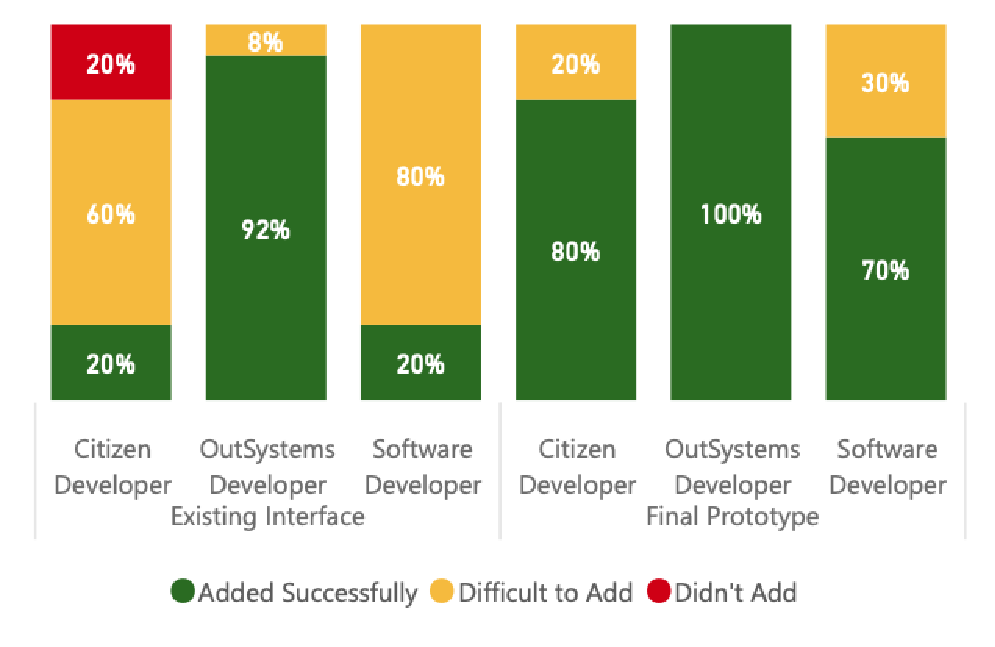
\includegraphics[width=0.5\linewidth]{add-calculated-attribute-comparison}}%
    \subcaptionbox{Left join with null readability\label{fig:leftJoinWithNullComparison}}%
    {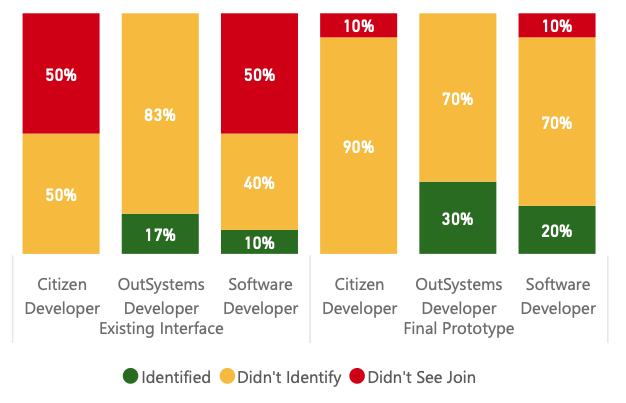
\includegraphics[width=0.5\linewidth]{left-join-with-null-readability-comparison}}%
    \\
  \subcaptionbox{Foreign key selection\label{fig:foreignKeySelectionComparison}}%
  {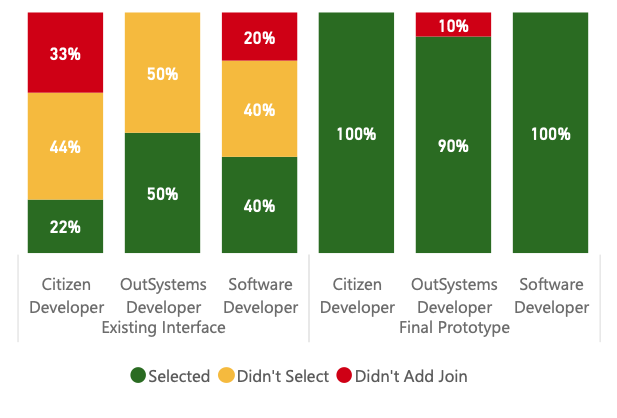
\includegraphics[width=0.5\linewidth]{foreign-key-selection-comparison}}%
  \subcaptionbox{Foreign key readability\label{fig:foreignKeyReadabilityComparison}}%
  {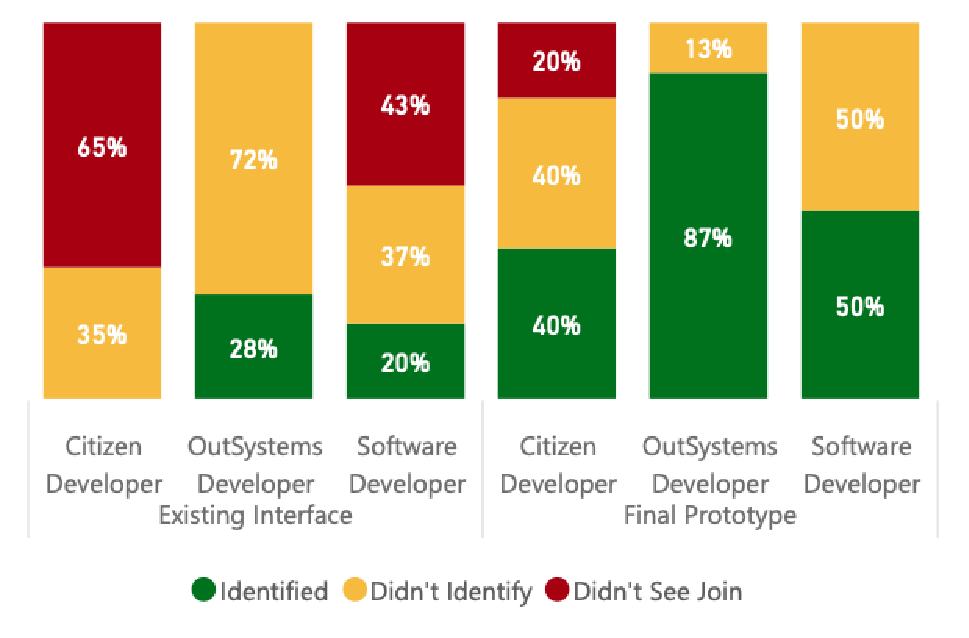
\includegraphics[width=0.5\linewidth]{foreign-key-readability-comparison}}%
  \caption{Comparison of the effectiveness between the Existing Interface and the Final Prototype, regarding specific use cases.}
  \label{fig:specificComparisons}
\end{figure}

% Please add the following required packages to your document preamble:
% \usepackage{booktabs}
\begin{table}[tb]
  \caption{Options used by users to insert the calculated attribute in the context of the M1 scenario. (Final Prototype usability tests - 30 users)}
  \label{tab:finalPrototypeOptionCalculatedAttribute}
  \begin{tabular}{@{}m{4.4cm}R{3.1cm}R{3.1cm}R{3.1cm}@{}}
  \toprule
  \textbf{Option used to insert the calculated attribute} & \multicolumn{1}{m{3.1cm}}{Add button on the bottom of the Sources View} & \multicolumn{1}{m{3.1cm}}{Right click in the attributes tree (Sources View)} & \multicolumn{1}{m{3.1cm}}{Add button on the result table (after all attributes)} \\ \midrule
  OutSystems Developer                                    & 50.00\%                                                          & 20.00\%                                                                & 30.00\%                                                                   \\
  Software Developer                                      & 90.00\%                                                         & 10.00\%                                                                & 0.00\%                                                                    \\
  Citizen Developer                                       & 100.00\%                                                          & 0.00\%                                                               & 0.00\%                                                                    \\
  Total                                                   & 80.00\%                                                          & 10.00\%                                                                & 10.00\%                                                                    \\ \bottomrule
  \end{tabular}
  \end{table}




The results of all scenarios and all users were combined, in order to evaluate the differences of the success rate that users achieved with the existing interface and with the final prototype. Thereby, Figure \ref{fig:totalEffectivenessComparison} presents the average of the success rate, considering all user groups (defined in section \ref{subsec:user_groups}), all scenarios (described in Appendix \ref{app:user_testing_scenarios}) and the success rate labelling presented in table \ref{tab:effectiveness_states}.

The changes applied in the interface have leveraged the values of the success rate. In the existing interface only 36\% of the scenarios were completely achieved and in the final prototype the percentage of the scenarios completely achieved was 68\%.

\begin{figure}[htbp]
	\centering
	\includegraphics[height=2.2in]{total-effectiveness-comparison}
	\caption{Effectiveness Comparison between the existing interface and the final prototype. (Comparing the 30 users who tested the existing interface with the other 30 users who tested the final prototype)}
	\label{fig:totalEffectivenessComparison}
\end{figure}

\medskip

\textbf{Analysis of Variance (ANOVA)}

\medskip

Furthermore, two one-way analysis of variance (ANOVA) were performed to determine if there are statistically significant differences between the mean users' success rate and the mean users' fail rate, using the existing interface and the final prototype.

\textbf{Achieved Scenarios:} Accordingly, the first ANOVA was computed to determine if the users' success rate (based on the percentage of achieved scenarios - stats presented in table \ref{tab:statistical_summary_achieved}) means are statistically different between the existing interface and the final prototype.

\begin{center}
  H0 - "There is no significant difference between the mean of achieved scenarios rate, in the existing interface and in the final prototype"
\end{center}

A one-way ANOVA, between subjects, was conducted (table \ref{tab:anova_achieved} to compare if the mean between the samples are equal. In a 95\% confidence interval, the null hypothesis is rejected, meaning that the two means are statistically different between the two tests ($p-value = 1.24E-06 < 0,05$). Therefore, it can be concluded that there is a statistically significant difference in terms of the achieved scenarios between the existing interface and the final prototype tests.

Regarding the effect size, which is a measure for ANOVA that indicates the proportion of variance accounted by a factor (i.e., measuring how different the means really are). Since the ANOVA performed was a one-way ANOVA, the effect size is given by the eta-squared ($\eta^2$), calculated using the formula \ref{eq:effect-size-formula}:

\begin{equation}
  \label{eq:effect-size-formula}
  \eta^2 = \frac{SS_{between}}{SS_{between} + SS_{within}}
\end{equation}

Comparing the average of the success rate obtained by users in the existing interface, which was $\approx 0.3495$, with the one obtaining when users tested the final prototype, which was $\approx 0.6667$, it can be concluded that, not only, there is a statistical difference, as proved by the ANOVA analysis, but also the effect size, which is $\approx 0.3355 > 0.14$ indicates that there is a large effect. Thereby, the probability of a user achieve a higher success rate in the final prototype than in the existing interface is corroborated.

% Please add the following required packages to your document preamble:
% \usepackage{booktabs}
\begin{table}[tb]
  \caption{Summary of the statistically data regarding the \textbf{achieved scenarios} in the existing interface and in the final prototype.}
	\label{tab:statistical_summary_achieved}
  \begin{tabular}{@{}m{5cm}rrrr@{}}
  \toprule
  \textbf{Groups}                                   & \multicolumn{1}{l}{\textbf{Count}} & \multicolumn{1}{l}{\textbf{Sum}} & \multicolumn{1}{l}{\textbf{Average}} & \multicolumn{1}{l}{\textbf{Variance}} \\ \midrule
  Achieved scenarios rate on the existing interface & 30                        & 10.4857                 & 0.3495                      & 0.0519                       \\
  Achieved scenarios rate on the final prototype    & 30                        & 20.0000                 & 0.6667                      & 0.0511                       \\ \bottomrule
  \end{tabular}
  \end{table}

% Please add the following required packages to your document preamble:
% \usepackage{booktabs}
\begin{table}[tb]
  \caption{Analysis of Variance (ANOVA) of the \textbf{scenarios achieved} in the existing interface and in the final prototype.}
	\label{tab:anova_achieved}
  \begin{tabular}{@{}lllllll@{}}
  \toprule
  \textbf{Source of Variation} & \textbf{SS}                & \textbf{df}            & \textbf{MS}                & \textbf{F}                  & \textbf{P-value}             & \textbf{F crit}            \\ \midrule
  Between Groups               & \multicolumn{1}{r}{1.5087} & \multicolumn{1}{r}{1}  & \multicolumn{1}{r}{1.5087} & \multicolumn{1}{r}{29.2874} & \multicolumn{1}{r}{1.24E-06} & \multicolumn{1}{r}{4.0069} \\
  Within Groups                & \multicolumn{1}{r}{2.9878} & \multicolumn{1}{r}{58} & \multicolumn{1}{r}{0.0515} &                             &                              &                            \\ \midrule
  \textbf{Total}               & 4.4965                     & 59                     &                            &                             &                              &                            \\ \bottomrule
  \end{tabular}
  \end{table}

\textbf{Not achieved scenarios:}
Since the method used to classify the success rate of the users while they performed the usability tests was not only yes or no answers but three types (achieved, partially achieved, and not achieved), the opposite of the achieved analysis is not the not achieved. In that way, another ANOVA analysis was performed concerning the not achieved scenarios in order to measure if users could formulate and comprehend queries in a most effective way using the final prototype than with the existing interface way even if they made some mistakes. \footnote{If the mean of the not achieved scenarios is statistically different and lower, the users could achieved and partially achieved scenarios with a higher probability in the final prototype than using the existing interface.}

Therefore, the second ANOVA was used to determine the differences between the not achieved scenarios (stats presented in table \ref{tab:statistical_summary_not_achieved}) in the existing interface and the final prototype.

\begin{center}
  H0 - "There is no significant difference between the mean of not achieved scenarios rate, in the existing interface and in the final prototype"
\end{center}

A one-way ANOVA, between subjects, was conducted (table \ref{tab:anova_not_achieved} to compare if the mean between the samples are equal. In a 95\% confidence interval, the null hypothesis is rejected, meaning that the two means are statistically different between the two tests ($p-value = 5.08E-05 < 0,05$). Therefore, it can be concluded that there is a statistically significant difference in terms of the not achieved scenarios between the existing interface and the final prototype tests.

Comparing the average of the not achievement rate obtained by users in the existing interface, which was $\approx 0.4905$, with the one obtaining when users tested the final prototype, which was $\approx 0.2543$, it can be concluded that not only there is a statistical difference, as proved by the ANOVA analysis, but also the effect size, which is $\approx 0.2586 > 0.14$, indicates that there is a large effect. Thereby, the probability of a user not achieve the given scenarios in the final prototype is lower than in the existing interface. 

It was also verified that in the existing interface the average of the achieved scenarios ($\approx 0.3495$) was lower than the average of the not achieved scenarios ($\approx 0.4905$), but in the final prototype the average of the achieve scenarios ($\approx 0.6667$) was superior of the average of the not achieved scenarios ($\approx 0.2543$). By this means, users managed to most successfully comprehend and formulate queries using the final prototype than using the existing interface.



% Please add the following required packages to your document preamble:
% \usepackage{booktabs}
\begin{table}[tb]
  \caption{Summary of the statistically data regarding the \textbf{not achieved scenarios} in the existing interface and in the final prototype.}
	\label{tab:statistical_summary_not_achieved}
  \begin{tabular}{@{}m{5cm}rrrr@{}}
  \toprule
  \textbf{Groups}                                       & \multicolumn{1}{l}{\textbf{Count}} & \multicolumn{1}{l}{\textbf{Sum}} & \multicolumn{1}{l}{\textbf{Average}} & \multicolumn{1}{l}{\textbf{Variance}} \\ \midrule
  Not Achieved scenarios rate on the existing interface & 30                                 & 14.7143                          & 0.4905                               & 0.0516                                \\
  Not Achieved scenarios rate on the final prototype    & 30                                 & 7.6286                           & 0.2543                               & 0.0358                                \\ \bottomrule
  \end{tabular}
  \end{table}


  % Please add the following required packages to your document preamble:
% \usepackage{booktabs}
\begin{table}[tb]
  \caption{Analysis of Variance (ANOVA) of the \textbf{scenarios not achieved} in the existing interface and in the final prototype.}
	\label{tab:anova_not_achieved}
  \begin{tabular}{@{}lrrllll@{}}
  \toprule
  \textbf{Source of Variation} & \multicolumn{1}{l}{\textbf{SS}} & \multicolumn{1}{l}{\textbf{df}} & \textbf{MS}                & \textbf{F}                  & \textbf{P-value}             & \textbf{F crit}            \\ \midrule
  Between Groups               & 0.8837                          & 1                               & \multicolumn{1}{r}{0.8368} & \multicolumn{1}{r}{19.1610} & \multicolumn{1}{r}{5.08E-05} & \multicolumn{1}{r}{4.0069} \\
  Within Groups                & 2.5330                          & 58                              & \multicolumn{1}{r}{0.0437} &                             &                              &                            \\ \midrule
  \textbf{Total}               & 3.3697                          & 59                              &                            &                             &                              &                            \\ \bottomrule
  \end{tabular}
  \end{table}

\subsection{Efficiency}
\label{subsec:efficiency}
The time users spent in each scenario when they tested the existing interface and the final prototype was also evaluated in order to compare the usability efficiency attribute of the final prototype against the one of the existing interface. Figure \ref{fig:box-plots-duration} and Table \ref{tab:duration-stats} presents the statistical data extracted to analyze the distribution of the time elapsed in each scenario and their skewness along the different quartiles.

As detailed in Table \ref{tab:duration-stats-comparison}, the comparison of the results regarding comprehension scenarios shown that the median has decreased at least 34\% with the exception of the scenario C4, where the median has increased 20 seconds from the existing interface to the final prototype tests. The difference between the first and the third quartiles has also become shorter in the comprehension scenarios excluding the case of the scenario C3 where this difference has slightly increased (2.67\%). 

Also noteworthy was the results about the scenario C1. As it was the first scenario tested in the usability tests, the time users needed to perform the intended task reflected also the time needed to explore the system for the first time to understand the way it works. In this scenario, the median has decreased 33.98\% and the difference between the first and the third quartiles 52.50\%, which means that users required less time to understand the interface. In that way, not only users who explored the interface for the first time were faster in the new prototype, but also the users, who were already accustomed, to use the existing interface were faster reaching the task's goal in the new interface.

Furthermore, the median time spent in the last comprehension scenario performed by users in the usability tests has decreased 42.71\% and the difference between the first and the third quartiles 133\%, which indicates that after exploring the interface through some scenarios, users needed less time to comprehend the query. Thereby, the interface revealed promising results in terms of productivity, essentially after passing the initial learning phase.

From the edition and formulation point of view, the results revealed that in the first modification scenario the median has decreased 8.76\% and the difference between the first and the third quartiles 26.30\%. This result demonstrated the success of improving the visibility option to add a new calculated attribute, which made new users to spend less time searching for this option, promoting a decrease on variance.

The formulation scenario did not presented a huge difference in terms of efficiency in opposite of the values presented before, regarding effectiveness. The median has decreased 4.0\% and the difference between first and the third quartiles 0.67\%. However, as stated before, there were positive results in terms of effectiveness which confirms that the changes applied in the interface, have helped users to reach the formulation goals. Nevertheless, there is a lack of some training and some accelerators to improve this values. Since the usability tests were made without previous training, users have used the final prototype for the first time, which led to a negative impact in terms of efficiency metrics because they needed time to explore the interface. 

Even without implementing some accelerators, as shortcuts or search engines, the efficiency results of the final prototype were not worse than the ones of the existing interface. Moreover, in the existing interface, some users have already used the interface before. In opposite, all users who tested the final prototype, tested the interface for the first. In that way, they needed time to explore the interface. Considering these factors, the efficiency metrics remained stable, which is a positive indicator, since users needed the same time using the interface although they were less experienced. Also, these results could be optimized if users gained experience using the interface, mainly if the missing accelerators were further implemented.

The time needed to complete the last modification scenario (M4) has decreased also in the final prototype. The median has decreased 29.35\% and the difference between the first and the third quartiles 42.40\%.

In a nutshell, this analysis on efficiency optimization pointed out multiple indicators that revealed improvements, even without the presence of some accelerators as well as experience using the interface which could leverage the efficiency metrics to a superior level.


  \begin{figure}[h]
    \centering
    \includegraphics[width=1.0\textwidth]{duration-box-plots}
    \caption{Box plots of the time used by users in each scenario in the existing interface (E) and in the final prototype (F).}
    \label{fig:box-plots-duration}
  \end{figure}

% Please add the following required packages to your document preamble:
% \usepackage{booktabs}
\begin{table}[tb]
  \caption{Statistical information about the time users elapsed in each scenario in the existing interface and in the final prototype.}
	\label{tab:duration-stats}
  \begin{tabular}{@{}llrrrrr@{}}
  \toprule
  Scenario & Interface          & \multicolumn{1}{l}{Min} & \multicolumn{1}{l}{Q1} & \multicolumn{1}{l}{Median} & \multicolumn{1}{l}{Q3} & \multicolumn{1}{l}{Max} \\ \midrule
  C1       & Existing Interface & 0:01:01                 & 0:01:56                & 0:03:00                    & 0:04:50                & 0:09:03                 \\
           & Final Prototype    & 0:00:57                 & 0:01:23                & 0:01:59                    & 0:03:15                & 0:07:43                 \\ \midrule
  M1       & Existing Interface & 0:01:18                 & 0:02:20                & 0:03:37                    & 0:05:41                & 0:11:17                 \\
           & Final Prototype    & 0:01:31                 & 0:02:33                & 0:03:18                    & 0:05:01                & 0:08:33                 \\ \midrule
  C2       & Existing Interface & 0:01:00                 & 0:02:02                & 0:02:51                    & 0:04:05                & 0:05:03                 \\
           & Final Prototype    & 0:01:04                 & 0:02:09                & 0:03:11                    & 0:04:12                & 0:07:38                 \\ \midrule
  C3       & Existing Interface & 0:00:28                 & 0:01:03                & 0:01:21                    & 0:01:50                & 0:02:52                 \\
           & Final Prototype    & 0:00:21                 & 0:00:32                & 0:00:45                    & 0:01:39                & 0:03:24                 \\ \midrule
  F1       & Existing Interface & 0:03:26                 & 0:05:59                & 0:07:21                    & 0:09:44                & 0:14:16                 \\
           & Final Prototype    & 0:02:58                 & 0:04:48                & 0:07:03                    & 0:09:15                & 0:12:25                 \\ \midrule
  C4       & Existing Interface & 0:00:35                 & 0:01:27                & 0:01:40                    & 0:02:13                & 0:03:31                 \\
           & Final Prototype    & 0:00:33                 & 0:00:45                & 0:00:57                    & 0:01:10                & 0:03:22                 \\ \midrule
  M4       & Existing Interface & 0:00:15                 & 0:02:10                & 0:03:42                    & 0:05:34                & 0:14:12                 \\
           & Final Prototype    & 0:00:18                 & 0:02:18                & 0:02:37                    & 0:04:11                & 0:07:35                 \\ \bottomrule
  \end{tabular}
  \end{table}

% Please add the following required packages to your document preamble:
% \usepackage{booktabs}
% \usepackage[table,xcdraw]{xcolor}
% If you use beamer only pass "xcolor=table" option, i.e. \documentclass[xcolor=table]{beamer}
\begin{table}[tb]
  \caption{Comparison of the time elapsed in each scenario between the tests of the existing interface and the tests of the final prototype.}
	\label{tab:duration-stats-comparison}
  \begin{tabular}{@{}
  >{\columncolor[HTML]{FFFFFF}}l 
  >{\columncolor[HTML]{FFFFFF}}r 
  >{\columncolor[HTML]{FFFFFF}}r 
  >{\columncolor[HTML]{FFFFFF}}r 
  >{\columncolor[HTML]{FFFFFF}}r @{}}
  \toprule
  Scenario & \multicolumn{1}{l}{\cellcolor[HTML]{FFFFFF}Median Difference} & \multicolumn{1}{l}{\cellcolor[HTML]{FFFFFF}Percentage} & \multicolumn{1}{l}{\cellcolor[HTML]{FFFFFF}Q3-Q1 Difference} & \multicolumn{1}{l}{\cellcolor[HTML]{FFFFFF}Percentage} \\ \midrule
  C1       & -0:01:01                                                      & -33.98\%                                               & -0:01:32                                                     & -52.50\%                                               \\ \midrule
  M1       & -0:00:19                                                      & -8.76\%                                                & -0:00:53                                                     & -26.30\%                                               \\ \midrule
  C2       & 0:00:20                                                       & 11.40\%                                                & 0:00:03                                                      & 2.65\%                                                 \\ \midrule
  C3       & -0:00:36                                                      & -44.10\%                                               & -0:00:04                                                     & -8.65\%                                                \\ \midrule
  F1       & -0:00:18                                                      & -4.08\%                                                & -0:00:02                                                     & -0.67\%                                                \\ \midrule
  C4       & -0:00:43                                                      & -42.71\%                                               & -0:01:01                                                     & -133.33\%                                              \\ \midrule
  M4       & -0:01:05                                                      & -29.35\%                                               & -0:01:27                                                     & -42.40\%                                               \\ \bottomrule
  \end{tabular}
  \end{table}



\subsection{Satisfaction}
\label{subsec:satisfaction}
After completing all the testings, users filled out a System Usability Survey (SUS) \cite{system_usability_scale}, where they attributed a number from 1 to 5 to each one of the sentences presented in Table \ref{tab:sus_results} and Figure \ref{fig:susChartComparison}.

The users' satisfaction increased in all questions. The users reacted positively to the changes implemented into the prototype, revealing that the system was more pleasant and simple to use as well as more consistent than the previous interface. Namely, the questions below were the ones with the highest average increase:

\begin{itemize}
  \item "I thought there was too much inconsistency in this system" (improved 44.58\%)
  \item I found the system very cumbersome to use" (43.88\%)
  \item "I found the various functions in this system were well integrated" (40.0\%)
  \item "I found the system unnecessarily complex" (33.80\%)
  \item "I think that I would like to use this system frequently" (27.35\%) 
\end{itemize}

However, although the questions regarding learnability have improved in comparison to the existing interface, they do not show as relevant as the remaining questions.

Since the system learnability could be highly affected by the users' background, the information retrieved from the users' profile survey was analyzed in order to perceive if there is some degree of correlation between the technical knowledge and the satisfaction using the interface.

Therefore, a study was performed in order to evaluate if the relational databases knowledge could have a significant impact into the users' opinion about how visual query builder is easy to use.

In that way, a Kendall's Tau-a correlation test was performed to determine the correlation between the relational database knowledge and the perception about how easy is to use the system. The sampl considered the 30 users who tested the existing interface and the 30 users who tested the final prototype. 

\begin{center}
  H0 = "There is no correlation between the relational databases knowledge and the interface ease of use"
\end{center}

Table \ref{tab:kendall-test} presents the values necessary to calculate this correlation value. 

In a 95\% confidence interval, the null hypothesis was rejected for both cases, the existing interface and the final prototype, which means that users with more relational databases knowledge were more likely to find the system easy to use.

% Please add the following required packages to your document preamble:
% \usepackage{booktabs}
\begin{table}[tb]
  \caption{Kendall's Tau-a significance test.}
	\label{tab:kendall-test}
  \begin{tabular}{@{}lrr@{}}
  \toprule
  \textbf{Kendall's Tau-a}                              & \multicolumn{1}{l}{\textbf{Existing Interface}} & \multicolumn{1}{l}{\textbf{Final Prototype}} \\ \midrule
  $\alpha$                                                 & 0.05                                            & 0.05                                         \\ \midrule
  Sample size                                           & 30                                              & 30                                           \\ \midrule
  Combinatorial                                         & 435                                             & 435                                          \\ \midrule
  Number of discordant pairs                            & 104                                             & 52                                           \\ \midrule
  Number of concordant pairs                            & 331                                             & 383                                          \\ \midrule
  Tau ($\tau$)                                                   & 0.5218                                          & 0.7609                                       \\ \midrule
  Tau-Critical                                          & 0.218                                           & 0.218                                        \\ \midrule
  \textbf{Significant? (Tau \textgreater Tau-Critical)} & \textbf{Yes}                                    & \textbf{Yes}                                 \\ \bottomrule
  \end{tabular}
  \end{table}

In conclusion, all the analysis and comparisons made between the existing interface and the final prototype built in this dissertation shown that, there was a considering improvement regarding the task completion rate and in the time users needed to comprehend the queries, illustrated in the interface. However, there are an opportunities to improve in terms of efficiency, mainly for formulation tasks and also regarding learnability, since the relational databases foundations are important to find the system easy to use.

